%\documentclass[12pt,draftcls]{ucdavisthesis}
\documentclass[12pt]{ucdavisthesis}

% PLEASE READ THE MANUAL - ucdavisthesis.pdf (in the package installation directory)

%%%%%%%%%%%%%%%%%%%%%%%%%%%%%%%%%%%%%%%%%%%%%%%%%%%%%%%%%%%%%%%%%%%%%%%%
%                                                                      %
%               LATEX COMMANDS FOR DOCUMENT SETUP                      %
%                                                                      %
%%%%%%%%%%%%%%%%%%%%%%%%%%%%%%%%%%%%%%%%%%%%%%%%%%%%%%%%%%%%%%%%%%%%%%%%

%\usepackage{bookmark}
\usepackage[us,nodayofweek,12hr]{datetime}
\usepackage{graphicx}
\usepackage{color}
\usepackage{lineno}
\linenumbers*[1]
\usepackage{url}
\usepackage{amsmath}
\usepackage{rotating} 
\usepackage[bottom]{footmisc}
\usepackage{graphics}

\usepackage{color}
\definecolor{pinkred}{rgb}{1.0, 0.4, 0.4}
\usepackage[table]{xcolor}
%\usepackage[square,comma,numbers,sort&compress]{natbib}
%\usepackage{hypernat}
% Other useful packages to try
%\usepackage{amsmath}
%\usepackage{amssymb}
%
% Different fonts to try (uncomment only fontenc and one font at a time)
% (you may need to install these first)
%\usepackage[T1]{fontenc} %enable fontenc package if using one of the fonts below
%\usepackage[adobe-utopia]{mathdesign}
%\usepackage{tgschola}
%\usepackage{tgbonum}
%\usepackage{tgpagella}
%\usepackage{tgtermes}
%\usepackage{fourier}
%\usepackage{fouriernc}
%\usepackage{kmath,kerkis}
%\usepackage{kpfonts}
%\usepackage[urw-garamond]{mathdesign}
%\usepackage[bitstream-charter]{mathdesign}
%\usepackage[sc]{mathpazo}
%\usepackage{mathptmx}
%\usepackage[varg]{txfonts}

\hyphenation{dis-ser-ta-tion blue-print man-u-script pre-par-ing} %add hyphenation rules for words TeX doesn't know


%\renewcommand{\rightmark}{\scriptsize A University of California Davis\ldots \hfill Rev.~\#1.0 \quad Compiled: \currenttime, \today}
% a fancier running header that can be used with draftcls options

%%%%%%%%%%%%%%%%%%%%%%%%%%%%%%%%%%%%%%%%%%%%%%%%%%%%%%%%%%%%%%%%%%%%%%%%
%                                                                      %
%        DOCUMENT SETUP AND INFORMATION FOR PRELIMINARY PAGES          %
%                                                                      %
%%%%%%%%%%%%%%%%%%%%%%%%%%%%%%%%%%%%%%%%%%%%%%%%%%%%%%%%%%%%%%%%%%%%%%%%

\title          {Studying Regional Climate with Variable-Resolution CESM}
%Exact title of your thesis. Indicate italics where necessary by underlining or using italics. Please capitalize the first letter of each word that would normally be capitalized in a title.

\author         {Xingying Huang}
%Your full name as it appears on University records. Do not use initials.

\authordegrees  {B.S. (Wuhan University) 2010 \\
                 M.S. (Beijing Normal University) 2013}
%Indicate your previous degrees conferred.

\officialmajor  {Atmospheric Science}
%This is your official major as it appears on your University records.

\graduateprogram{Atmospheric Science}
%This is your official graduate program name. Used for UMI abstract.

\degreeyear     {2016}
% Indicate the year in which your degree will be officially conferred.

\degreemonth    {December}
% Indicate the month in which your degree will be officially conferred. Used for UMI abstract.

\committee{Professor Paul Ullrich, Chair}{Professor Terry Nathan}{Professor Daniel Feldman}{}{}
% These are your committee members. The command accepts up to five committee members so be sure to have five sets of braces, even if there are empties.

%%%%%%%%%%%%%%%%%%%%%%%%%%%%%%%%%%%%%%%%%%%%%%%%%%%%%%%%%%%%%%%%%%%%%%%%

%\copyrightyear{2020}
%\nocopyright

%%%%%%%%%%%%%%%%%%%%%%%%%%%%%%%%%%%%%%%%%%%%%%%%%%%%%%%%%%%%%%%%%%%%`%%%%

\dedication{\textsl{To someone very important \ldots \\
            a nice dedication.}}

%%%%%%%%%%%%%%%%%%%%%%%%%%%%%%%%%%%%%%%%%%%%%%%%%%%%%%%%%%%%%%%%%%%%%%%%

\abstract{Regional climate is becoming one of the most important areas under the umbrella of climate change research, as more information is now needed at finer scales.  High horizontal resolution is needed to allow a more accurate representation of fine scale forcing, and leads to a better representation of processes and interactions that are significantly drivers for regional and local climate variability. Regional climate models (RCMs) are a traditional method for modeling regional climate, and have been proven to be capable of both mean climate and extreme events studies. Over the past decade, variable-resolution global climate models (VRGCMs) have been introduced as an alternative way for studying regional climate and applications. In this research, the newly developed variable-resolution technique within the Community Earth System Model (CESM) has been applied for long-term regional climate studies. 

In this thesis, firstly, VR-CESM is assessed for long-term regional climate modeling over California against a traditional RCM -- the Weather Research and Forcasting (WRF) model. Mean historical climatology has been analyzed and contrasted with reanalysis, gridded observational datasets. Overall, VR-CESM produced comparable statistical biases to WRF in key climatological quantities. Generally, when compared with gridded observational datasets, both VR-CESM and WRF adequately represented regional climatological patterns. VR-CESM demonstrated competitive utility for studying high-resolution regional climatology when compared to a regional climate model (WRF). This assessment highlights the value of variable-resolution global climate models (VRGCMs) in capturing fine-scale atmospheric processes, projecting future regional climate and addressing the computational expense of uniform-resolution global climate models.

Supported by the satisfactory performances from the previous evaluation of the VR-CESM in regional climate modeling, VR-CESM is further applied to understand the impact of irrigation on the regional climate of California. Irrigation is an important contributor to the regional climate of heavily irrigated regions, and within the U.S. there are few regions that are as heavily irrigated as California's Central Valley. A flexible irrigation scheme with relatively realistic estimates of agricultural water use is employed and the impact of irrigation on mean historical climatology and heat extremes is investigated. It turns out that high-resolution simulations of regional climate in CESM, particularly over heavily irrigated regions, should likely enable the irrigation parameterization to better represent local temperature statistics.

Based on VR-CESM, which proves to be a useful tool for regional climate studies, we have also investigated the projected changing character of precipitation frequency and intensity in the western United States over the 21st century. Both mean changes to precipitation and distributions of both non-extreme and extreme events, projected by the VR-CESM model under climate forcing, have been investigated.  Although constrained by water influx and soil moisture, changes to extreme precipitation are hypothesized to follow the Clausius-Clapeyron relationship more closely than total precipitation amount. We aim to add value to the study of regional climate change through the use of a reliable model to reduce uncertainty in predicting changes to both mean climatology and extremes. We expect these studies can contribute to the characterization, detection and attribution of mean climatology and precipitation extremes at multi-scale.}

%{The abstract submitted as part of your dissertation, in the introductory pages, does not have a word limit. It should follow the same format as the rest of your dissertation (1.5 inch left margin, double-spaced, consecutive page numbering, etc.).}

%%%%%%%%%%%%%%%%%%%%%%%%%%%%%%%%%%%%%%%%%%%%%%%%%%%%%%%%%%%%%%%%%%%%%%%%

\acknowledgments{Over all these years, there are a lot help I have received from numerous people, who have contributed significantly to the completion of this thesis. First of all, I would like to thank my advisor, Paul Ullrich, for his support and inspiration through all my Ph.D. studies. Many thanks go to my research group fellow Alan M. Rhoades for helping in modeling work and collaborating in part of my research work. I would also like to offer thanks to the many collaborators I have had the pleasure of working for the past three years, in particular, Colin M. Zarzycki at NCAR.

Specifically, for the work in chapter 2, I would like to thank Dr. Travis O'Brien for the many useful conversations on climate model assessment. We also want to thank Xue Meng Chen for her assistance in performing the WRF simulations. As for chapter 3, I'd like to thank Dr. Travis O'Brien, Dr. Richard Grotjahn and Dr. Graham E. Fogg for many useful suggestions. We would also like to thank IT support for our local UC Davis computing cluster. Lastly, for chapter 4, I would like to thank Michael Wehner for sharing the 0.25$^\circ$ uniform-resolution CESM dataset, and his many suggestions. The authors also want to thank Alan M. Rhoades for providing the simulation output and providing his feedback on the content.

Special thanks go to all the friends I have met at the University of California, Davis with whom I have experienced a lot enjoyable moments. They are Shaoyun, Marielle, Xuemeng, Jing and many others who have been my good company. Thanks for all of you showing me the joy of life. I also want to thank my best friends and the beloved ones for all the unforgettable memory.

Most importantly, I would like to thank my family for their support and encouragement all the way. Without them, I cannot get through all the difficulties I have come across all these years. Special thanks go to my father and mother, who have tried their best to provide me what I need and raised me up to where I am today.}

%Acknowledgements to those who helped you get to this point. They should be listed by chapter when appropriate.

%%%%%%%%%%%%%%%%%%%%%%%%%%%%%%%%%%%%%%%%%%%%%%%%%%%%%%%%%%%%%%%%%%%%%%%%

% Each chapter can be in its own file for easier editing and brought in with the \include command.
% Then use the \includeonly command to speed compilation when working on a particular chapter.
%%% \includeonly{ucdavisthesis_example_Chap1}

\begin{document}

\newcommand{\bibfont}{\singlespacing}
% need this command to keep single spacing in the bibliography when using natbib

\bibliographystyle{agufull08}
%\bibliographystyle{unsrtnat}
%many other bibliography styles are available (IEEEtran, mla, etc.). Use one appropriate for your field.

\makeintropages %Processes/produces the preliminary pages

\chapter{Introduction}

\section{Background}

Global climate models (GCMs) have been widely used to simulate both past and future climate. Although these models have demonstrable success in representing large-scale features of the climate system, they are usually employed at relatively coarse resolutions ($\sim$1$^\circ$), largely as a result of the substantial computational cost required at higher resolutions. Global climate reanalysis datasets, which assimilate climate observations using a global model, represent a best estimate of historical weather patterns. However, reanalysis datasets still cannot fulfill the needs of policymakers, stakeholders and researchers that require high-resolution regional climate data (\url{http://reanalyses.org/atmosphere/overview-current-reanalyses}). Regional features such as microclimates, land cover, and topography, are not well captured by either GCMs or reanalysis datasets \cite{leung2003regional}.However, dynamical processes at unrepresented scales are significant drivers for local climate variability, especially over complex terrain \cite{soares2012wrf}. In order to capture fine-scale dynamical features, high horizontal resolution is needed for a more accurate representation of small-scale processes and interactions \cite{rauscher2010resolution}. With these enhancements, regional climate data is expected to be more useful for formulating climate adaptation and mitigation strategies locally.

In order to model regional climate at high spatial resolutions over a limited area, downscaling techniques have been developed, such as statistical and dynamical downscaling. Dynamical downscaling typically uses nested limited-area models (LAMs) or, more recently, variable-resolution enabled GCMs (VRGCMs) \cite{laprise2008regional}. In this context, LAMs are typically referred to as regional climate models (RCMs) when used for climate study. Forced by the output from GCMs or reanalysis datasets, RCMs have been widely used to capture physically consistent regional and local circulations at the needed spatial and temporal scales \cite{christensen2007regional, bukovsky2009precipitation, mearns2012north}. Recently, there has been a growing interest in the use of VRGCMs for modeling regional climate. Unlike RCMs, VRGCMs use a relatively coarse global model with enhanced resolution over a specific region \cite{staniforth1978variable, fox1997finite}.  Strategies that have been employed for transitioning between coarse and fine-resolution regions within a VRGCM include grid stretching \cite{fox1997finite, mcgregor2008updated} and grid refinement \cite{ringler2008multiresolution, skamarock2012multiscale, zarzycki2014aquaplanet}. VRGCMs have demonstrated utility for regional climate studies and applications at a reduced computational cost compared to uniform-resolution GCMs \cite{fox2006variable, rauscher2013exploring, zarzycki2015effects}. 

Compared with RCMs, a key advantage of VRGCMs is that they use a single, unified modeling framework, rather than two separate models (GCM and RCM) with potentially disparate dynamics and physics parameterizations. RCMs may suffer from potential inconsistencies between the global and regional scales and lack two-way interactions at the nest boundary \cite{warner1997tutorial, mcdonald2003transparent, laprise2008challenging, mesinger2013limited}, which can be mitigated with the use of VRGCMs. VRGCMs also provide a cost-effective method of reaching high resolutions over a region of interest -- the limited area simulations in this study at 0.25$^\circ$ and 0.125$^\circ$ resolution represent a reduction in required computation of approximately 10 and 25 times, respectively, compared to analogous globally uniform high-resolution simulations. For the purposes of this paper, we focus on the recently developed Community Earth System Model with variable-resolution option (VR-CESM) as our VRGCM of interest. This configuration is driven by the Community Atmosphere Model's (CAM's) Spectral Element (SE) dynamical core, which possesses attractive conservation and parallel scaling properties \cite{dennis2011cam, taylor2011conservation}, as well as recently developed variable-resolution capabilities \cite{zarzycki2014aquaplanet, zarzycki2015experimental}. This model has been employed by \cite{zarzycki2014using} to show that a high-resolution refinement patch in the Atlantic basin for simulating topical cyclones represented significant improvements over the unrefined simulation. \cite{zarzycki2015effects} also compared the large-scale climatology of VR-CESM 0.25$^\circ$ and uniform CESM at 1$^\circ$, and found that adding a refined region over the globe did not noticeably affect the global circulation. \cite{rhoades2015characterizing} has also assessed the use of VR-CESM for modeling Sierra Nevada mountain snowpack in the western United States.

Irrigation effects are usually ignored in climate models for several reasons: irrigation usually occurs over a relatively small area ($\sim$2$\%$ of global land surface) and produces a seemingly negligible cooling effect compared to global greenhouse warming \cite{boucher2004direct}. Nonetheless, irrigation is a potentially important factor in regulating climate patterns at regions scales, where there is a growing need for accurate climate assessments and projections. Past studies have typically addressed the climatic effects of irrigation in limited-area models (LAMs) \cite{snyder2006regional, kueppers2007irrigation}, which in the context of climate modeling are typically referred to as regional climate models (RCMs). In these studies, irrigation is modeled by accounting for the amount of irrigated water needed and the area of cropland where irrigation is applied. Using a multi-model ensemble of RCM simulations, \cite{kueppers2008seasonal} found that the behavior of RCMs varied in representing effects of irrigation on regional climate, depending on each model's physics, as well as on the configuration of the irrigation parameterization.

California is the most irrigated state in the U.S., and most of California's irrigated cropland is distributed over the Central Valley (CV), which is responsible for 25$\%$ of domestic agricultural products \cite{wilkinson2002potential}. Irrigation is an important contributor to the regional climate of heavily irrigated regions, and within the U.S. there are few regions that are as heavily irrigated as California's Central Valley, responsible for 25$\%$ of domestic agricultural products. In order to model regional climate over the CV, relatively fine horizontal resolution is needed to more accurately represent microclimates, land-use, small-scale dynamical features and corresponding interactions \cite{leung2003regional, rauscher2010resolution}.  There is a need to study the impact of irrigation on regional climate over the CV, based on VR-CESM, which features a more flexible irrigation scheme with relatively realistic estimates of regional agricultural water use.

There is substantial and growing interest in understanding the character of precipitation within a changing climate, motivated largely by its pronounced impacts on water availability and flood management in both human and natural systems \cite{hegerl2004detectability, kharin2007changes, scoccimarro2013heavy}.  Among past studies addressing precipitation, extremes have been a major focus, particularly drought and flood events \cite{seneviratne2012changes}.  Overall, it is widely agreed that although atmospheric water vapor concentration is increasing, the impacts of a changing climate on the character of precipitation is far more complicated.  Extreme precipitation events are particularly nuanced:  Our best projections suggest that extreme precipitation events will intensify even in regions where mean precipitation decreases \cite{tebaldi2006going, kharin2007changes}.

Although several past studies have investigated climate extremes at the global scale \cite{seneviratne2012changes}, studies addressing extremes at local and regional scales are less common. It is well understood how increased GHG concentrations have contributed to the observed intensification of heavy precipitation events over the tropical ocean \cite{allan2008atmospheric} and the majority of Northern Hemisphere overland areas \cite{min2011human}, but changes are much more poorly understood at regional scales where meteorological variability is large \cite{trenberth2011changes}. This issue of insufficient regional-scale climate information has been a major outstanding problem in climate science, as stakeholders and water managers typically require fine-scale information on climate impacts in order to effectively develop adaptation and mitigation strategies. 

The western United States (WUS) area is known to be particularly vulnerable to hydrological extremes, particularly floods and droughts \cite{leung2003hydroclimate, caldwell2010california}, and hosts a variety of local features and microclimates associated with its rough and varied topography. It is important to understand the changes in the character of precipitation, in terms of frequency and intensity, from recent history through the end of the 21st century over WUS.

\section{Outline of Thesis}

In this thesis, regional climate has been studied from past to future over western United States (especially, California), working with VR-CESM--the newly developed variable-resolution enabled Community Earth System Model. This thesis is organized as follows. In Chapter 2, VR-CESM is assessed for long-term regional climate modeling over California against a traditional RCM -- the Weather Research and Forcasting (WRF) model. We aim to fill that gap by analyzing the performance of VR-CESM against gridded observational data, reanalysis product and in comparison to a traditional RCM forced by reanalysis data. This chapter focuses on the models' ability to represent current climate statistics, particularly those relevant to heat and precipitation extremes. In Chapter 3, VR-CESM is further applied to understand the impact of irrigation on the regional climate of California. A flexible irrigation scheme with relatively realistic estimates of agricultural water use is employed and the impact of irrigation on mean historical climatology and heat extremes is investigated. In Chapter 4, the projected changing character of precipitation in the western United States over the 21st century has been investigated under the RCP 8.5 ``business-as-usual'' scenario. Both mean changes to precipitation and distributions of both non-extreme and extreme events, projected by the VR-CESM model under climate forcing, have been studied. A concise conclusion is given in the last chapter.

%\chapter{An Evaluation of the Variable Resolution-CESM for Modeling California's Climate}
%

% Enter your Abstract here
\section{Abstract}

In this chapter, the recently developed variable-resolution option within the Community Earth System Model (VR-CESM) is assessed for long-term regional climate modeling of California at $0.25^\circ$ ($\sim$28 km) and $0.125^\circ$ ($\sim$14 km) horizontal resolutions. The mean climatology of near-surface temperature and precipitation is analyzed and contrasted with reanalysis, gridded observational datasets and a traditional regional climate model (RCM) -- the Weather Research and Forcasting (WRF) model. Statistical metrics for model evaluation and tests for differential significance have been extensively applied. With only prescribed sea surface temperatures, VR-CESM tended to produce a warmer summer (by about 1 to 3 $^\circ$C) and overestimated overall winter precipitation (about 25$\%$-35$\%$) compared to reference datasets. Increasing resolution from 0.25$^\circ$ to 0.125$^\circ$ did not produce a statistically significant improvement in the model results. By comparison, the analogous WRF climatology (constrained laterally and at the sea surface by ERA-Interim reanalysis) was $\sim$1 to 3 $^\circ$C colder than the reference datasets, underestimated precipitation by $\sim$20$\%$-30$\%$ at 27 km resolution and overestimated precipitation by $\sim$65-85$\%$ at 9 km.  Overall, VR-CESM produced comparable statistical biases to WRF in key climatological quantities.  This assessment highlights the value of variable-resolution global climate models (VRGCMs) in capturing fine-scale atmospheric processes, projecting future regional climate and addressing the computational expense of uniform-resolution global climate models.


% MAIN BODY OF PAPER
\section{Introduction}

Global climate models (GCMs) have been widely used to simulate both past and future climate. Although these models have demonstrable success in representing large-scale features of the climate system, they are usually employed at relatively coarse resolutions ($\sim$1$^\circ$), largely as a result of the substantial computational cost required at higher resolutions. Global climate reanalysis datasets, which assimilate climate observations using a global model, represent a best estimate of historical weather patterns. However, reanalysis datasets still cannot fulfill the needs of policymakers, stakeholders and researchers that require high-resolution regional climate data (\url{http://reanalyses.org/atmosphere/overview-current-reanalyses}). Regional features such as microclimates, land cover, and topography, are not well captured by either GCMs or reanalysis datasets \cite{leung2003regional}.However, dynamical processes at unrepresented scales are significant drivers for local climate variability, especially over complex terrain \cite{soares2012wrf}. In order to capture fine-scale dynamical features, high horizontal resolution is needed for a more accurate representation of small-scale processes and interactions \cite{rauscher2010resolution}. With these enhancements, regional climate data is expected to be more useful for formulating climate adaptation and mitigation strategies locally.

In order to model regional climate at high spatial resolutions over a limited area, downscaling techniques have been developed, such as statistical and dynamical downscaling. Dynamical downscaling typically uses nested limited-area models (LAMs) or, more recently, variable-resolution enabled GCMs (VRGCMs) \cite{laprise2008regional}. In this context, LAMs are typically referred to as regional climate models (RCMs) when used for climate study. Forced by the output from GCMs or reanalysis datasets, RCMs have been widely used to capture physically consistent regional and local circulations at the needed spatial and temporal scales \cite{christensen2007regional, bukovsky2009precipitation, mearns2012north}. Recently, there has been a growing interest in the use of VRGCMs for modeling regional climate. Unlike RCMs, VRGCMs use a relatively coarse global model with enhanced resolution over a specific region \cite{staniforth1978variable, fox1997finite}.  Strategies that have been employed for transitioning between coarse and fine-resolution regions within a VRGCM include grid stretching \cite{fox1997finite, mcgregor2008updated} and grid refinement \cite{ringler2008multiresolution, skamarock2012multiscale, zarzycki2014aquaplanet}. VRGCMs have demonstrated utility for regional climate studies and applications at a reduced computational cost compared to uniform-resolution GCMs \cite{fox2006variable, rauscher2013exploring, zarzycki2015effects}. 

Compared with RCMs, a key advantage of VRGCMs is that they use a single, unified modeling framework, rather than two separate models (GCM and RCM) with potentially disparate dynamics and physics parameterizations. RCMs may suffer from potential inconsistencies between the global and regional scales and lack two-way interactions at the nest boundary \cite{warner1997tutorial, mcdonald2003transparent, laprise2008challenging, mesinger2013limited}, which can be mitigated with the use of VRGCMs. VRGCMs also provide a cost-effective method of reaching high resolutions over a region of interest -- the limited area simulations in this study at 0.25$^\circ$ and 0.125$^\circ$ resolution represent a reduction in required computation of approximately 10 and 25 times, respectively, compared to analogous globally uniform high-resolution simulations. For the purposes of this paper, we focus on the recently developed Community Earth System Model with variable-resolution option (VR-CESM) as our VRGCM of interest. This configuration is driven by the Community Atmosphere Model's (CAM's) Spectral Element (SE) dynamical core, which possesses attractive conservation and parallel scaling properties \cite{dennis2011cam, taylor2011conservation}, as well as recently developed variable-resolution capabilities \cite{zarzycki2014aquaplanet, zarzycki2015experimental}. This model has been employed by \cite{zarzycki2014using} to show that a high-resolution refinement patch in the Atlantic basin for simulating topical cyclones represented significant improvements over the unrefined simulation. \cite{zarzycki2015effects} also compared the large-scale climatology of VR-CESM 0.25$^\circ$ and uniform CESM at 1$^\circ$, and found that adding a refined region over the globe did not noticeably affect the global circulation. \cite{rhoades2015characterizing} has also assessed the use of VR-CESM for modeling Sierra Nevada mountain snowpack in the western United States.


However, for the purposes of long-term regional climate modeling, particularly in regions where high-resolution is anticipated to be most beneficial, VR-CESM has yet to be rigorously evaluated. This paper aims to fill that gap by analyzing the performance of VR-CESM against gridded observational data, reanalysis product and in comparison to a traditional RCM forced by reanalysis data. Our variable-resolution simulations are implemented with horizontal resolutions of 0.25$^\circ$ and 0.125$^\circ$ respectively, which are much more typical for dynamically downscaled studies. This paper focuses on California in the western United States as the study area. The complex topography and coastlines of California strongly modulate large-scale weather patterns, creating local climatic features such as coastal fog, sea breeze, mountain-induced precipitation and snowpack. An understanding of local climate variability in California is incredibly important for policymakers and stakeholders due to its vast agricultural industry, mixed demographics, and vulnerability to anthropogenically-induced climate change \cite{hayhoe2004emissions, cayan2008overview}.  Consequently, we expect that California is an excellent test bed for regional climate modeling.


In this study the Weather Research and Forecasting (WRF) \cite{skamarock2005coauthors} model has been used for simulating California's climatology at 27km and 9km grid spacing. RCM simulations over California have also been conducted in previous studies and demonstrated the need for high spatial and temporal resolution to better address regional climate and extreme events, especially in the vicinity of complex topography where large climatological gradients are present \cite{leung2004mid, kanamitsu2007fifty, caldwell2009evaluation, pan2011influences, pierce2013probabilistic}. In particular, \cite{caldwell2009evaluation} presented results from WRF at 12km spatial resolution and showed that, although the RCM was effective at simulating the mean climate when compared with observations, some clear biases persisted (particularly an overestimation of precipitation).

This study focuses on the models' ability to represent current climate statistics, particularly those relevant to heat and precipitation extremes. We anticipate that this work will validate VR-CESM for modeling the mean regional climatology of California and will further motivate the adoption of variable-resolution modeling to study other local climatic processes. Our eventual goal is to utilize these models for assessing historical and future regional climate extremes.

This paper is organized as follows: Section 2 describes the model setup, datasets and methodology for evaluation and intercomparison. In section 3, simulation results are provided and discussed, with focuses on near-surface (2-meter) temperature and precipitation. Key results are summarized along with further discussion in section 4.

\section{Models and Methodology}

\subsection{Simulation design} 

In this study, all global simulations use the Atmospheric Model Intercomparison Project (AMIP) experimental protocols \cite{Gates1992}. These protocols are widely used and support climate model diagnosis, validation and intercomparison. AMIP experiments are constrained by realistic sea-surface temperatures (SSTs) and sea ice from 1979 to near present without the added complexity of ocean-atmosphere feedbacks in the climate system. In particular, observed SSTs and sea ice at 1$^\circ$ horizontal resolution are provided and updated following the procedure described by \cite{hurrell2008new}.

\subsubsection{VR-CESM}

CESM is a state-of-the-art Earth modeling framework managed by the National Center for Atmospheric Research (NCAR), consisting of coupled atmospheric, oceanic, land and sea ice models.  For decades CESM (and its predecessor, the Community Climate System Model) has been used for modeling present and future global climate \cite{neale2010description, hurrell2013community}.  The coupling infrastructure in CESM communicates the interfacial states and fluxes between each component model to ensure conservation. Since we follow AMIP protocols, only the atmosphere and land model are integrated dynamically. Here, CAM version 5 (CAM5) \cite{CAM5Tech} and the Community Land Model (CLM) version 4.0 \cite{CLM40Tech} are used. As mentioned earlier, the SE dynamical core is employed along with variable-resolution grid support. The FAMIPC5 (F$\_$AMIP$\_$CAM5) component set, which mainly supports atmospheric, oceanic, land and sea ice models, is chosen for these simulations. In CAM5, cloud microphysics is parameterized using the two-moment scheme with with ice supersaturation \cite{ morrison2008new, gettelman2008new}, and the deep convection process is treated by Zhang and McFarlane (ZM) cumulus scheme \cite{zhang1995sensitivity}. A more detailed discussion of the CAM5 configuration can be found in \cite{neale2010description}.

For our study, the variable-resolution cubed-sphere grids are generated for use in CAM and CLM with the open-source software package SQuadGen \cite{ullrich2014squadgen,guba2014spectral}. The grids used in this study are depicted in Figure \ref{fig:Figure 1}.  The maximum horizontal resolution on these grids is 0.25$^\circ$ ($\sim$28km) and 0.125$^\circ$ ($\sim$14km) respectively, with a quasi-uniform 1$^\circ$ mesh over the remainder of the globe. Grids are constructed using a paving technique with a 2:1 spatial resolution ratio, so two transition layers are required from 1$^\circ$ to 0.25$^\circ$, and one additional transition from 0.25$^\circ$ to 0.125$^\circ$. In our study, and previous studies (e.g. \cite{zarzycki2015effects}), general circulation patterns (e.g., wind, pressure and precipitation) do not exhibit apparent artifacts in the variable-resolution transition region, and the design of the SE dynamical core ensures that dry air and tracer mass are conserved globally \cite{taylor2010compatible}. Simulations are performed over the time period from 1979-01-01 to 2005-12-31 (UTC) and year 1979 is discarded as a spin-up period. This 26-year time period is chosen to provide an adequate sampling of inter-annual variability, to limit computational cost, and to coincide with the satellite era where adequate high-quality gridded and reanalysis datasets are available.

%Figure 2.1
\begin{figure}
\begin{center}
\includegraphics[width=6in]{worldmap_modified.pdf}
\caption{The approximate grid spacing in the (a) VR-CESM 0.25$^\circ$ and (b) VR-CESM 0.125$^\circ$ meshes used in this study. (c) A depiction of the transition from the global $1^\circ$ resolution mesh through two layers of refinement to $0.25^\circ$ and again to $0.125^\circ$.}
\label{fig:Figure 1}
\end{center}
\end{figure}
%%%%%%%


Variable-resolution topography files were produced by sampling the National Geophysical Data Center (NGDC) 2-min ($\sim$4 km) Gridded Global Relief Dataset (ETOPO2v2), followed by the application of a differential smoothing technique as described in \cite{zarzycki2015effects}.  Using this technique, the $c$ parameter from their Eq. (1) was adjusted to reduce noise in the vertical pressure velocity field. The grid-scale topography is depicted in Figure \ref{fig:Figure 2}, including the topography of uniform CESM at 1$^\circ$ and observed topography from USGS 2 minute (~3 km) dataset. Hypsometric curves, depicting the percentage of the California region above a given elevation, are plotted in Figure \ref{fig:Figure 2} for models and observations. It is apparent that higher resolution provides clear improvement in the representation of regional topography, which is necessary for the correct treatment of fine-scale dynamic processes strongly influenced by complex terrain. Topography at very coarse resolution ($\sim$1$^\circ$) is too smooth to represent local details like the shape of valleys or mountain peaks, resulting in the loss of regional climate patterns.

Land surface datasets, including plant functional types, at $0.5$$^\circ$ were adopted. Greenhouse gas (GHG) concentrations and aerosol forcings are prescribed based on historical observations. CAM and CLM tuning parameters are not modified from their default configurations.

%Figure 2.2
\begin{figure}
\begin{center}
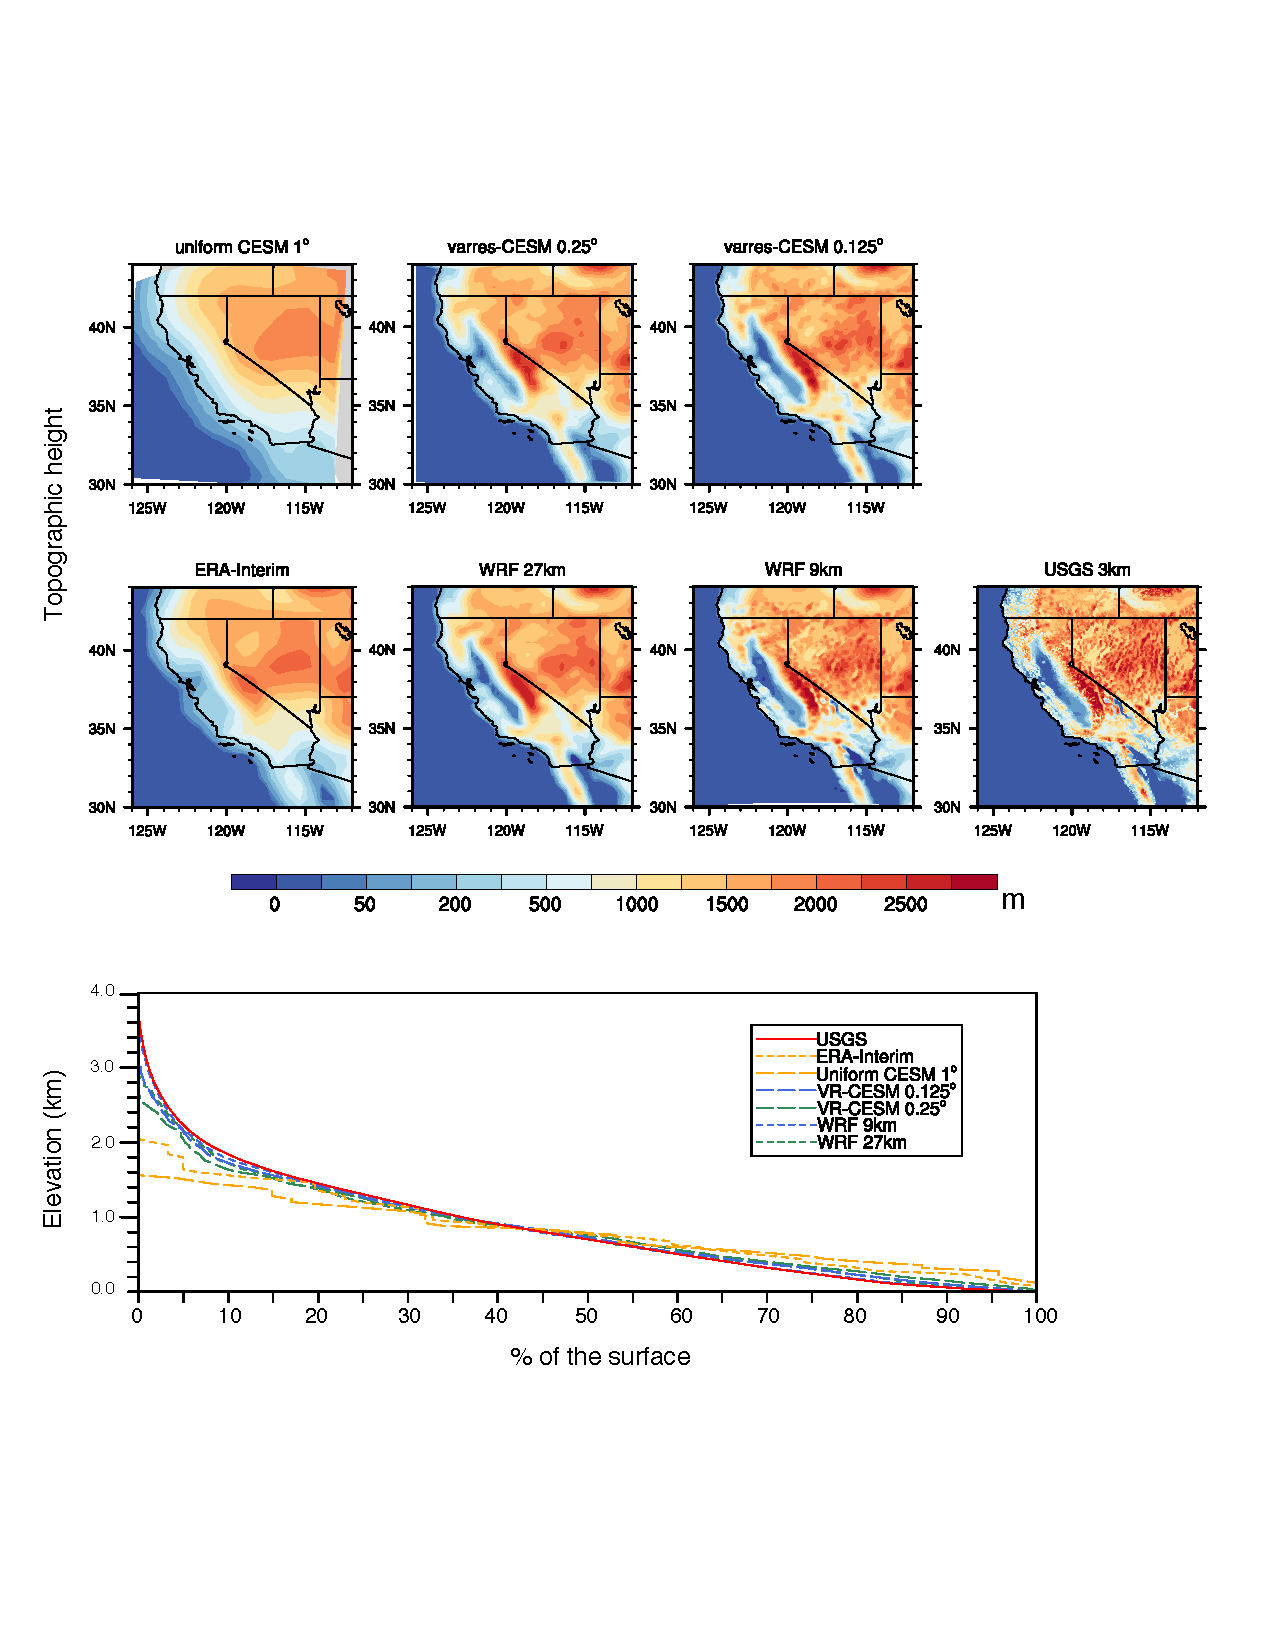
\includegraphics[width=6in]{topo.pdf}
\end{center}
\caption{Upper panel: Topographic heights (from top left to bottom right) for VR-CESM 0.25$^\circ$, VR-CESM 0.125$^\circ$, uniform CESM 1$^\circ$, WRF 27km, WRF 9km, ERA-Interim ($\Delta x \sim$80 km) and USGS ($\sim$3 km); Lower panel: Hypsometric curves for the above datasets over California.} \label{fig:Figure 2} 
\end{figure}
%%%%%%%%%

\subsubsection{WRF} 

WRF has been widely used over the past decade for modeling regional climate \cite{lo2008assessment, leung2009atmospheric, soares2012wrf, sun2015hybrid}. In our study, the fully compressible non-hydrostatic WRF model (version 3.5.1) with the Advanced Research WRF (ARW) dynamical core is used.  WRF is a limited area model that supports nested domains with a typical refinement ratio of 3:1.  The simulation domains of WRF are depicted in Figure \ref{fig:Figure 3}. Two WRF simulations, representing finest grid resolutions of 27 km and 9 km, are conducted.  For the WRF 27km simulation, one domain is used. For the WRF 9km simulation, two domains are used, with the outer domain at 27 km (same as the WRF 27km) and an inner nested domain at 9 km horizontal grid resolution. For both simulations,  grids are centered on California and have 120$\times$110 and 151$\times$172 grid points, respectively. At all lateral boundaries, 10 grid points are used for relaxation to the coarse solution. In order to reduce the drift between forcing data and modeling output, grid nudging \cite{stauffer1990use} is applied to the outer domain every 6 hours at all levels except approximate planetary boundary layers (PBL), as suggested by \cite{lo2008assessment}. The nudging is applied to the wind, temperature and water vapor mixing ratio with default nudging coefficients. Grid nudging is commonly used and maturely supported in WRF. Although there is evidence spectral nudging may improve the quality of the simulations, an investigation of these differences is out of scope for this paper \cite{liu2012differences}. This setup uses 41 vertical levels with model top pressure at 50 hPa.

%Figure 2.3
\begin{figure}
\begin{center}
\includegraphics[width=6in]{wrf_domains.pdf}
\end{center}
\caption{Left: WRF 27km (entire plot region) and WRF 9km (solid black box) simulation domains; Right: five climate divisions for California.  Both plots are overlaid with WRF model topography.} \label{fig:Figure 3}
\end{figure}
%%%%%%%%

Additionally, the following physics parameterizations are employed: WSM (WRF Single-Moment) 6-class graupel microphysics scheme \cite{hong2006wrf}, Kain-Fritsch cumulus scheme \cite{kain2004kain}, CAM shortwave and longwave radiation schemes \cite{collins2004description}.  These settings are chosen by assessing the results from several common parameterization combinations over a one-year trial period, which were then compared to gridded observations. For the boundary layer, the Yonsei University scheme (YSU) \cite{hong2006new} is used, and the Noah Land Surface Model \cite{chen2001coupling} is applied. Both are chosen as they are common for climate applications that balance long-term reliability and computational cost.  Although many other options and parameterization combinations are available for configuring WRF (and others have tackled a complete assessment of these options for particular problems), our choices are made simply to represent a typical WRF configuration. We do note that the Kain-Fritsch convective parameterization remains active even within the 9km inner mesh -- although this is considered to be in the ``gray zone'', it had no appreciable impact on  simulation results since almost all precipitation emerged from (large-scale) condensation, as discussed in Section 4.

ECMWF Reanalysis (ERA-Interim) data at both the surface and multiple pressure-levels provides initial and lateral conditions for the domains. The lateral conditions and SSTs are updated every 6 hours. ERA-Interim reanalysis ($\sim$80 km) has been widely used and validated for its reliability as forcing data \cite{dee2011era}. WRF simulations are conducted over the same time period as VR-CESM (i.e., 1979-01-01 through 2005-12-31 UTC). Again, the year 1979 is used as a spin-up period and is discarded for purposes of analysis. Notably, the $\sim$9 km resolution employed in the innermost domain is finer than most previous studies for long-term climate.

The topography employed for the 27 km and 9 km simulations is interpolated from USGS (United States Geological Survey) elevation data with 10-min ($\sim$20 km) and 2-min ($\sim$4 km) resolution, respectively. The post-processed grid-scale topography is contrasted in Figure \ref{fig:Figure 2}. Elevation differences between VR-CESM and WRF are irregular and relatively small, except over the Central Valley where VR-CESM has consistently higher values than WRF. This indicates a different methodology for preparation of the topography dataset and may also be partly due to the use of the USGS elevation instead of NGDC elevation datasets. 

\subsection{Gridded and Reanalysis Datasets}

Reanalysis and gridded observational datasets of the highest available quality are employed (see Table \ref{tab:Datasets}). Differences between gridded observations can be due to the choice of meteorological stations, interpolation techniques, elevation models and processing algorithms.  Consequently, the use of multiple reference datasets is necessary to understand the underlying uncertainty in the observational data.  Detailed descriptions of these datasets are as follows.

\paragraph{NARR}  The North American Regional Reanalysis (NARR) is the NCEP (National Centers for Environmental Prediction) high-resolution reanalysis product that provides dynamically downscaled data over North America at $\sim$32 km resolution and 3-hourly intervals from 1979 through present \cite{mesinger2006north}. We note that some inaccuracies have also been identified in NARR, particularly in precipitation fields \cite{bukovsky2007brief}.

\paragraph{NCEP CPC} This dataset provides gauge-based analysis of daily precipitation from the National Oceanic and Atmospheric Administration (NOAA) Climate Prediction Center (CPC). It is a suite of unified precipitation products obtained by combining all information available at CPC via the optimal interpolation objective analysis technique. The gauge analysis covers the Conterminous United States with a fine-resolution at 0.25$^\circ$ from 1948-01-01 to 2006-12-31.


\paragraph{PRISM} The Parameter-elevation Regressions on Independent Slopes Model (PRISM) \cite{daly2008physiographically} supports a 4 km gridded dataset obtained by taking point measurements and applying a weighted regression scheme that accounts for many factors affecting the local climatology. The datasets include total precipitation and minimum/maximum, (derived) mean temperatures and dewpoints. Monthly climatological variables are available for 1895 through 2014 from the PRISM Climate Group (Oregon State University, \url{http://prism.oregonstate.edu}, created 4 Feb 2004). Notably, PRISM is the United States Department of Agriculture's official climatological dataset.  PRISM is used as our primary reference dataset for model performance evaluation.

\paragraph{UW} The UW daily gridded meteorological data is obtained from the Surface Water Modeling group at the University of Washington \cite{maurer2002long, hamlet2005production}. UW incorporates topographic corrections by forcing the long-term average precipitation to match that of the PRISM dataset. The temperature dataset is produced in a similar fashion as precipitation, but uses a simple 6.1 K/km lapse rate for topographic effect. The dataset is provided at 0.125$^\circ$ horizontal resolution covering the period 1949 to 2010.


\paragraph{Daymet}  Daymet is an extremely high resolution (1 km) gridded dataset with daily outputs of total precipitation, humidity, and minimum/maximum temperature covering 1980 through 2013 \cite{thornton1997generating, thornton2014daymet}. The dataset is produced using an algorithmic technique that ingests point station measurements in conjunction with a truncated Gaussian weighting filter.  Some adjustments are made to account for topography. Daymet is available through the Oak Ridge National Laboratory Distributed Active Archive Center (ORNL DAAC). 

%table 2.1
\begin{table}
\caption{Reanalysis and gridded observational datasets used in this study.} \label{tab:Datasets}
\begin{center}
\begin{tabular}{lccccc} 
\hline \textbf{Data source} & \textbf{Variables used} & \textbf{Spatial resolution} & \textbf{Temporal resolution} \\
\hline \textbf{NARR} & Pr, T$_{s}$ & 32 km & daily, 3-hourly \\
\textbf{NCEP CPC} & Pr & $\sim$28 km (0.25$^\circ$) & daily \\
\textbf{UW} & Pr, T$_{min}$, T$_{max}$ & $\sim$14 km (0.125$^\circ$) & daily \\
\textbf{PRISM} & Pr, T$_{min}$, T$_{max}$, T$_{avg}$ & 4 km & monthly \\
\textbf{Daymet} & Pr, T$_{min}$, T$_{max}$ & 1 km & daily \\
\hline
\end{tabular}
\end{center}
\end{table}
%%%%%%%%%%

\subsection{Methodology}

Near-surface temperature and precipitation have been analyzed over California to assess the performance of VR-CESM in representing the mean climatology. Specifically, our evaluation focuses on daily maximum, minimum and average near-surface temperatures (T$_{max}$, T$_{min}$ and T$_{avg}$) and daily precipitation (Pr). These variables are key in a baseline climate assessment due to their close relationship with water resources, agriculture and health. In this context, the biggest impact of weather on California is through heat and precipitation extremes. Since heat extremes dominate during the summer season, we focus on June, July and August (JJA) for assessment of temperature. On the other hand, since the vast majority of precipitation in California occurs in the winter season, December-January-February (DJF) is emphasized.  

In order to adequately account for natural variability of the mean climate, the simulation period must be chosen appropriately \cite{solomon2007climate}. However, the number of simulated years required for adequate climate statistics depends greatly on the regional climate variability and spatial scale. Past studies have used average weather conditions over a 30-year period to ensure sufficient statistics and to avoid imprinting from annual variability \cite{dinse2009climate}. To check that our 26-year simulation period is sufficient, we have examined the interannual variability of mean temperature and precipitation in all simulations and observations over 5, 10, 20 and 25 seasons or years (depicted in the supplemental figures). We observe that for climatological mean temperature and precipitation, the relevant statistics are effectively converged for a 20-year sample, suggesting that our simulation period is sufficient to adequately capture the interannual variability of these quantities. 


The results in section 4 are obtained from simulated and observed data over the period 1980 to 2005.  All datasets have been linearly de-trended at each grid point so as to facilitate averaging of all simulation years. It is found that, for annual and JJA near-surface temperature (T$_{max}$, T$_{min}$ and T$_{avg}$), a statistically significant trend is present under the two-tailed t-statistic with a significance level of 0.05. For T$_{min}$, the average warming in 26 years is $\sim$0.6 K$-$1 K for observations, $\sim$0.5 K for VR-CESMs and WRF 27km and $\sim$1.5 K for WRF 9km. For T$_{max}$, the average warming is $\sim$0.3 K$-$0.5 K for observations, $\sim$0.5 K$-$0.8 K for VR-CESMs and WRFs. No statistically significant trend has been detected for precipitation.

California consists of a diverse variety of climate regions as a consequence of its rugged topography and large latitudinal extent.  The distinct character of these regions is poorly captured in typical coarse global climate simulations \cite{abatzoglou2009classification, caldwell2009evaluation}.  In order to assess the performance of VR-CESM within each region, the state has been divided into five climate divisions, including the Central Valley (CV), Mountain Region (MR), North Coast (NC), South Coast (SC), and Desert Region (DR).  The spatial extent of these divisions is depicted in Figure \ref{fig:Figure 3}. These five divisions are determined loosely based on the results of \cite{abatzoglou2009classification} and the climate divisions used by the California Energy Commission. To restrict the analysis in each division, simulations and datasets have been masked to restrict climate variables to each division. 


Standard statistical measures have been used to quantify the model performance in comparison with the reference datasets. These include the root-mean-square deviation (RMSD), mean signed difference (MSD), mean relative absolute difference (MRD), and sample standard deviation ($s$). Further, spatial correlation is assessed by computing Pearson product-moment coefficient of linear correlation between climatological means from models and reference datasets.  Mathematically, these quantities are written as
\begin{align}
RMSD &= \sqrt{\frac{1}{N} \sum_{i=1}^{N} (v_i - \hat{v}_i)^2}  & MSD &= \frac{1}{N} \sum_{i=1}^{N} (v_i - \hat{v}_i) \\[2.0ex]
s &= \sqrt{\frac{1}{M-1} \sum_{j=1}^{M} (v_j - \bar{v})^2}   & MRD &= \left( \sum_{i=1}^{N} |v_i - \hat{v}_i| \right) \Bigg/ \left( \sum_{i=1}^{N} \hat{v}_i \right).
\end{align} where $v_i$ and $\hat{v}_i$ are values from the simulation output and reference dataset, respectively; $i$ is the grid-point index and N is the total number of grid points over specific regions; $j$ is the simulation year index, M is the total number of simulated years and $\bar{v}$ is the mean value over all years. Grid-point differences are calculated by remapping the reference datasets to the model's output grid using bilinear interpolation.  Remapping using patch-based interpolation has also been tested and nearly identical results have been observed.  When necessary, the statistical quantities are further averaged over each division.


Throughout the remainder of this paper, student's t-test has been used to test whether two sets of annual-, seasonal- or monthly-averaged data are the same. F-test is applied to test whether the sample variances are equal. These tests are used only when the sample population can be described adequately by a normal distribution, where normality is assessed under the Anderson-Darling test. When the sample populations do not approximately follow a normal distribution, Mann-Whitney-Wilcoxon (MWW) test and Levene's test are employed in lieu of the t-test and F-test, respectively. All statistical tests are evaluated at the $p = 0.05$ significance level.

Complementary results to this study are provided in the online supplement, including the original grid-refined mesh files, the sensitivity of climatological statistics to choice of time period, the observed time trend, and other seasons not addressed in this paper and corresponding statistics metric tables. Results are also provided with comparison of VR-CESM to the output from a globally uniform CESM run at 0.25$^\circ$ spatial resolution with the finite volume (FV) dynamical core \cite{wehner2014effect}.

\subsection{Uncertainty in Reference Products}

To assess uncertainty in the observational and reanalysis products, we have calculated the MSD values among PRISM, UW and Daymet for seasonally averaged JJA T$_{max}$, T$_{min}$ and DJF Pr over the five divisions and tabulated these results in Table \ref{tab:stat_Datasets}. Student's t-test is employed to determine significances of differences. For T$_{max}$ and T$_{min}$, gridded observational datasets are different from each other over some divisions.  The most pronounced divergences occur in the NC region, with MSD values reaching up to $\sim$4$^\circ$C, although differences are also apparent for MR T$_{min}$. Clearly, UW and Daymet have a colder climatology than PRISM. NARR, as a reanalysis dataset, is different from the others over most divisions, with overall larger T$_{min}$ and smaller T$_{max}$. For precipitation, essentially no significant differences are present, especially among PRISM, UW and Daymet. NARR and CPC (not shown) seem to have slightly lower precipitation values than others.

%table 2.2
\begin{table}
\caption{MSD (left column minus top row) of JJA temperature ($^\circ$C) and DJF precipitation (mm/day) between all reference datasets. Statistically significant differences are emphasized (95\% confidence level).} \label{tab:stat_Datasets}
\begin{tabular}{lccccccccccccccccc}
\hline \textbf{JJA T$_{min}$} & \multicolumn{5}{c}{\textbf{PRISM}} & & \multicolumn{5}{c}{\textbf{UW}} & & \multicolumn{5}{c}{\textbf{Daymet}} \\
\hline & MR &CV& DR& SC& NC & & MR& CV &DR &SC& NC & & MR &CV &DR &SC& NC \\
\hline \textbf{UW} & \textbf{\color{pinkred}-2.0} & \textbf{\color{pinkred}-0.5} & -0.3 & \textbf{\color{pinkred}-0.4} & \textbf{\color{pinkred}-2.3} \\
\textbf{Daymet} & \textbf{\color{pinkred}-1.8} & 0.2 & -0.2 & -0.3 & \textbf{\color{pinkred}-4.6} & & 0.2 & \textbf{\color{pinkred}0.8} & 0.1 & 0.1 & \textbf{\color{pinkred}-2.3} \\
\textbf{NARR} & \textbf{\color{pinkred}2.5} & \textbf{\color{pinkred}2.5} & \textbf{\color{pinkred}3.1} & -0.2 & \textbf{\color{pinkred}2.0} & & \textbf{\color{pinkred}4.5} & \textbf{\color{pinkred}3.1} & \textbf{\color{pinkred}3.4} & 0.2 & \textbf{\color{pinkred}4.2} & & \textbf{\color{pinkred}4.3} & \textbf{\color{pinkred}2.3 }& \textbf{\color{pinkred}3.2} & 0.1 & \textbf{\color{pinkred}6.5} \\
\hline \hline \textbf{JJA T$_{max}$} & \multicolumn{5}{c}{\textbf{PRISM}} & & \multicolumn{5}{c}{\textbf{UW}} & \multicolumn{5}{c}{\textbf{Daymet}} \\
\hline & MR &CV& DR& SC& NC & & MR& CV &DR &SC& NC & & MR &CV &DR &SC& NC \\
\hline \textbf{UW} & 0.3 & -0.1 & -0.2 & \textbf{\color{pinkred}-0.7} & \textbf{\color{pinkred}-2.4} \\
\textbf{Daymet} & -0.3 & 0.4 & -0.2 & 0.2 & \textbf{\color{pinkred}-3.7} & & -0.6 & \textbf{\color{pinkred}0.5} & 0.1 & \textbf{\color{pinkred}0.9} & \textbf{\color{pinkred}-1.3} \\
\textbf{NARR} & \textbf{\color{pinkred}-1.3} & \textbf{\color{pinkred}1.2} & -0.1 & \textbf{\color{pinkred}-0.6} & \textbf{\color{pinkred}-3.7} & & \textbf{\color{pinkred}-1.7} & \textbf{\color{pinkred}1.2} & 0.1 & 0.1 & \textbf{\color{pinkred}-1.3} & & \textbf{\color{pinkred}-1.1} & \textbf{\color{pinkred}0.7} & 0.1 & \textbf{\color{pinkred}-0.7} & 0.0 \\
\hline \hline \textbf{DJF Pr} & \multicolumn{5}{c}{\textbf{PRISM}} & & \multicolumn{5}{c}{\textbf{UW}} & & \multicolumn{5}{c}{\textbf{Daymet}} \\
\hline & MR &CV& DR& SC& NC & & MR& CV &DR &SC& NC & & MR &CV &DR &SC& NC \\
\hline \textbf{UW} & -0.2 & 0.1 & 0.0 & -0.2 & -0.2 \\
\textbf{Daymet} & -0.1 & -0.4 & -0.0 & 0.2 & 0.5 & & 0.1 & -0.5 & -0.0 & 0.3 & 0.8 \\
\textbf{NARR} & -0.5 & -0.4 & -0.1 & -0.1 &\textbf{\color{pinkred}-1.3} & & -0.3 & -0.5 & -0.1 & 0.1 & -1.1 & & -0.4 & -0.0 & -0.1 & -0.3 & \textbf{\color{pinkred}-1.8} \\ 
\textbf{CPC} & -0.8 & 0.0 & 0.0 & -0.1 & -1.1 & & -0.5 & -0.1 & 0.0 & 0.1 & -0.9 & & -0.6 & 0.4 & 0.0 & -0.3 & \textbf{\color{pinkred}-1.7} \\
\hline
\end{tabular}
\end{table}
%%%%%%%%%%

\section{Results}

A detailed analysis of temperature and precipitation results from WRF and VR-CESM is provided in this section.  A concise summary of key points follows in section \ref{sec:Discussion}.

\subsection{Temperature}

The mean JJA T$_{max}$, T$_{min}$ and T$_{avg}$ climatology over the simulation period, together with PRISM and NARR reference data, is plotted in Figure \ref{fig:Figure 4}. UW and Daymet have not been plotted here since they are visually indistinguishable to PRISM everywhere except for NC, where UW and Daymet exhibit lower temperatures (see Table \ref{tab:stat_Datasets}).  Statistical measures over California are tabulated in Table \ref{tab:stat_JJA_t2}. In general, all simulations have captured the spatial climate patterns exhibited by PRISM, with high spatial correlations ($>$0.95), especially for T$_{max}$ and T$_{avg}$.  Nonetheless, several clear biases (relative to PRISM) are present in these simulations, as discussed below.

%Figure 2.4
\begin{figure}
\begin{center}
\includegraphics[width=6in]{t2_JJA.pdf}
\end{center}
\caption{JJA averaged daily T$_{max}$, T$_{min}$ and T$_{avg}$ from models and reference datasets, and differences (sharing the same legend) between model results and PRISM.} \label{fig:Figure 4}
\end{figure}
%%%%%%%%

%table 2.3
\begin{table}
\begin{center}
\caption{RMSD ($^\circ$C), MSD ($^\circ$C) and Spatial Correlation (Corr) for seasonally-averaged daily JJA temperatures over California. } \label{tab:stat_JJA_t2}
\begin{tabular*}{5.5in}{l @{\extracolsep{\fill}}ccccccccc}
\hline \textbf{RMSD} & \multicolumn{2}{c}{\textbf{UW}}  & & \multicolumn{3}{c}{\textbf{PRISM}} & & \multicolumn{2}{c}{\textbf{Daymet}} \\
\hline & T$_{max}$ &  T$_{min}$ & & T$_{max}$ & T$_{min}$ & T$_{avg}$& & T$_{max}$ & T$_{min}$\\
\hline \textbf{VR-CESM 0.25$^\circ$} & 2.32 & 3.75 & & 2.92 & 3.12 & 2.60 & & 2.81 & 3.93 \\
\textbf{VR-CESM 0.125$^\circ$} \quad & 1.90 & 3.63 & & 2.45 & 2.94 & 2.18 & & 2.48 & 3.70 \\
\textbf{WRF 27km} & 2.31 & 2.74 & & 2.93 & 2.25 & 2.17 & & 2.51 & 2.99 \\
\textbf{WRF 9km} & 3.32 & 2.94 & & 3.49 & 1.84 & 1.77 & & 3.20 & 2.94 \\
\textbf{Uniform CESM 1$^\circ$} & 3.06 & 4.59 & & 3.62 & 3.43 & 3.16 & & 3.58 & 5.07 \\
\hline \hline \textbf{MSD} & \multicolumn{2}{c}{\textbf{UW}}  & & \multicolumn{3}{c}{\textbf{PRISM}} & & \multicolumn{2}{c}{\textbf{Daymet}} \\\hline & T$_{max}$ &  T$_{min}$ && T$_{max}$ & T$_{min}$ & T$_{avg}$&& T$_{max}$ &  T$_{min}$\\
\hline \textbf{VR-CESM 0.25$^\circ$} & 0.98 & 2.91 & & 0.61 & 1.73 & 0.82 & & 1.18 & 2.88 \\
\textbf{VR-CESM 0.125$^\circ$} \quad & 0.65 & 2.85 & & 0.20 & 1.66 & 0.58 & & 0.82 & 2.74 \\
\textbf{WRF 27km} & -0.58 & 0.82 & & -0.95 & -0.36 & -0.77 & & -0.39 & 0.79 \\
\textbf{WRF 9km} & -2.28 & 1.86 & & -2.72 & 0.67 & -1.14 & & -2.10 & 1.76 \\
\textbf{Uniform CESM 1$^\circ$} & 0.82 & 3.03 & & 0.60 & 1.76 & 1.08 & & 1.24 & 3.38 \\
\hline \hline \textbf{Corr} & \multicolumn{2}{c}{\textbf{UW}}  & & \multicolumn{3}{c}{\textbf{PRISM}} & & \multicolumn{2}{c}{\textbf{Daymet}} \\\hline & T$_{max}$ &  T$_{min}$ && T$_{max}$ & T$_{min}$ & T$_{avg}$&& T$_{max}$ &  T$_{min}$\\
\hline \textbf{VR-CESM 0.25$^\circ$} & 0.99 & 0.98 & & 0.99 & 0.98 & 0.99 & & 0.99 & 0.97 \\
\textbf{VR-CESM 0.125$^\circ$} \quad & 0.99 & 0.98 & & 0.99 & 0.98 & 0.99 & & 0.99 & 0.98 \\
\textbf{WRF 27km} & 0.99 & 0.98 & & 0.99 & 0.98 & 0.99 & & 0.99 & 0.97 \\
\textbf{WRF 9km} & 0.99 & 0.98 & & 0.99 & 0.99 & 0.99 & & 0.99 & 0.98 \\
\textbf{Uniform CESM 1$^\circ$} & 0.99 & 0.96 & & 0.99 & 0.97 & 0.99 & & 0.99 & 0.95 \\
\hline
\end{tabular*}
\end{center}
\end{table}
%%%%%%%%%%%

\begin{itemize}
\item{} \textbf{T$_{max}$:}  When compared with the reference datasets, VR-CESM showed a warm bias of about 2 to 3 $^\circ$C in T$_{max}$ over much of the inland domain (CV and MR) and a 2 to 3 $^\circ$C cool bias along the coast, although the coastal bias is reduced by $\sim$0.5 $^\circ$C at 0.125$^\circ$ resolution. This is in contrast with WRF, which produced an overall colder climate everywhere except the CV.  This bias is especially pronounced for the WRF 9km simulation, which was approximately 3 $^\circ$C cooler than PRISM. T$_{max}$ within the CV has been overestimated by all the simulations. This likely represents a systematic issue with high-resolution models with respect to California.  Possible reasons for this overestimation are discussed at the end of this section.


\item{} \textbf{T$_{min}$:}  VR-CESM showed a strong warm bias in T$_{min}$ ($\sim$2 to 4 $^\circ$C), with a particularly large overestimation over Nevada ($> 5 ^\circ$C). WRF also exhibited a warm bias, but of a much smaller magnitude ($\sim$2 to 3 $^\circ$C). However, the pattern of T$_{min}$ presented in Figure \ref{fig:Figure 4} in both WRF simulations suggests a cooler interior to the CV and warmer perimeter, which is not supported by observations.

\item{} \textbf{T$_{avg}$:}  The warm bias of T$_{min}$ and T$_{max}$ by VR-CESM resulted in a similar overestimation of T$_{avg}$. For WRF, underestimation of T$_{max}$ and overestimation of T$_{min}$ led to an overall closer match to T$_{avg}$ over most of the domain, but is indicative of a suppressed diurnal cycle.
\end{itemize}

Compared with the reference datasets over California, VR-CESM 0.125$^\circ$ produced the lowest RMSD values for T$_{max}$, whereas WRF had smallest RMSD for T$_{min}$.  However, in both cases the RMSD was around 2 $^\circ$C.  Notably, T$_{min}$ from VR-CESM matched much more closely with NARR, although this is likely indicative of a related warm bias in NARR.  In fact, closer examination of the differences among VR-CESM, WRF and NARR marine near-surface temperature patterns indicated that CESM and NARR have T$_{min}$ values that are approximately 2 $^\circ$C larger than WRF.  Since coastal near-surface temperature is strongly influenced by ocean SSTs, this difference is likely a key driver of the warm bias in CESM. The Delta breeze effect, which is associated with a sea breeze circulation that brings relatively cool and humid marine air into the interior CV from the San Francisco Bay area, was apparent in all runs. It is especially encouraging that VR-CESM generally performed as well as WRF, in comparison with reference datasets, even though VR-CESM was not constrained or nudged at the lateral boundaries of the high-resolution domain.

The spatial standard deviation of JJA T$_{max}$, T$_{min}$ and T$_{avg}$ from models and PRISM is presented in Figure \ref{fig:Figure 5}. In PRISM, the CV had smaller variability than surrounding regions, although the difference is small ($\sim$0.2 $^\circ$C). Further, areas with rougher topography did exhibit somewhat higher variability than smoother locations. Interestingly, the higher resolution (0.125$^\circ$) VR-CESM simulation also matched the spatial pattern and magnitude of standard deviation observed in PRISM, especially for T$_{min}$ and T$_{avg}$. However, in WRF and VR-CESM 0.25$^\circ$, the variability is largely consistent across different divisions, and the values are around 0.5 to 1.5 $^\circ$C for all of the datasets, except for the high Sierras in the WRF 9km simulation which showed enhanced variability ($\sim$2 $^\circ$C). Compared with reference datasets, the RMSD values of VR-CESM and WRF 27km are $\sim$0.1-0.2 $^\circ$C, and $\sim$0.2-0.3 $^\circ$C for WRF 9km.

%Figure 2.5
\begin{figure}
\begin{center}
\includegraphics[width=6in]{t2_JJA_std.pdf}
\end{center}
\caption{Sample standard deviation of JJA average daily T$_{max}$, T$_{min}$ and T$_{avg}$ from model results and PRISM.} \label{fig:Figure 5}
\end{figure}
%%%%%%%%%%

The seasonal cycle of monthly mean T$_{avg}$ in each division is shown in Figure \ref{fig:Figure 6} for simulations and for reference data from PRISM and NARR along with the associated 95\% confidence interval. PRISM and NARR match closely almost everywhere except in the summer season of NC, SC and CV, indicative of underlying observational uncertainty. This difference is likely due to the discrepancy in assimilating the coastal cooling effect.  In general, model results match closely with reference data with no larger than a 2 $^\circ$C absolute difference, with the largest errors occurring in the summer and winter seasons.  Compared with PRISM, VR-CESM overpredicts summer T$_{avg}$ in all divisions except NC and SC, and underpredicts winter T$_{avg}$ in all divisions.  This corresponds to a larger annual temperature range. WRF has better performance in preserving the monthly cycle when compared with VR-CESM, with about 1 $^\circ$C underestimation over all seasons. There is no clear improvement in the seasonal cycle across resolutions.

%Figure 2.6
\begin{figure}
\begin{center}
\includegraphics[width=6in]{trd_t2avg_allzones.pdf}
\end{center}
\caption{Seasonal cycle of monthly-average T$_{avg}$ for each climate division. The shading corresponds to the 95\% confidence interval of PRISM and NARR. } \label{fig:Figure 6}
\end{figure}
%%%%%%%%%%%

Variability in monthly-averaged T$_{avg}$ is expressed by the interannual standard deviation of monthly T$_{avg}$ over the 26-year period and is plotted in Figure \ref{fig:Figure 7} for the whole California region (results are similar for sub-regions when renormalized by the mean T$_{avg}$). The 95\% confidence interval obtained from the Chi-square test is also depicted for PRISM so as to identify statistically significant differences.  RMSD values for monthly standard deviations between models and PRISM are also computed over each climate division (see Table \ref{tab:stat_std}). Generally, standard deviation is between 1 to 2 $^\circ$C. Among all models, WRF 27km is closest to PRISM with RMSD values around 0.1-0.2 $^\circ$C. WRF 9km is also relatively close to PRISM, but exhibits an unusual $\sim$1 $^\circ$C increase in variability in January and February (statistically significant at the 0.05 level), leading to a relatively high RMSD ($\sim$0.5 $^\circ$C). VR-CESM exhibits a weaker correlation with PRISM in all divisions with enhanced variability in DJF and weakened variability in April and May at both resolutions, and in the fall season in the 0.125$^\circ$ simulation, with RMSD around 0.2-0.4 $^\circ$C.  This may be indicative of an issue in capturing the seasonality of large-scale Pacific meteorology in CESM and merits further investigation.

%Figure 2.7
\begin{figure}
\begin{center}
\includegraphics[width=6in]{trd_t2avg_pr_std.pdf}
\end{center}
\caption{Standard deviation values of monthly-average T$_{avg}$ and Pr averaged over California. The shading refers to the 95\% confidence interval of PRISM. } \label{fig:Figure 7}
\end{figure}
%%%%%%%%%

%table 2.4
\begin{table}
\begin{center}
\caption{RMSD for the standard deviation values of monthly-averaged T$_{avg}$/Pr between models and PRISM in each climate division.}
\label{tab:stat_std}
\begin{tabular*}{5.5in}{l @{\extracolsep{\fill}}ccccc}
\hline \textbf{T$_{avg}$} & \textbf{MR}  & \textbf{CV}  & \textbf{DR} & \textbf{SC} & \textbf{NC} \\
\hline \textbf{VR-CESM 0.25$^\circ$}  & 0.393 & 	0.304 & 	0.231 & 	0.253 & 	0.286  \\
\textbf{VR-CESM 0.125$^\circ$} &  0.468 & 	0.355	&  0.359 & 	0.275 & 	0.334 \\
\textbf{WRF 27km} &  0.101 & 	0.199 & 	0.129 & 	0.231 & 	0.141 \\
\textbf{WRF 9km}  &  0.438 & 	0.561 & 	0.454 & 	0.476 & 	0.536 \\
\hline
\end{tabular*}

\begin{tabular*}{5.5in}{l @{\extracolsep{\fill}}ccccc}
\hline \textbf{Pr} & \textbf{MR}  &  \textbf{CV} & \textbf{DR} & \textbf{SC} & \textbf{NC} \\
\hline \textbf{VR-CESM 0.25$^\circ$} & 0.449 &	 0.976 &	0.228 &	0.517 &	0.670 \\
\textbf{VR-CESM 0.125$^\circ$}  & 0.315 &	0.848	 &  0.237	& 0.532 &	0.499 \\
\textbf{WRF 27km}  & 0.193 &	0.126  &	0.246  &	0.494  &	0.724  \\
\textbf{WRF 9km}  & 1.700  &	1.057  &	0.425  &	 0.817  &	0.958 \\
\hline
\end{tabular*}

\end{center}
\end{table}
%%%%%%%%%%%

Due to the impact of summer heat waves, we now focus on T$_{max}$ over JJA. In Figure \ref{fig:Figure 8}, the frequency distribution of T$_{max}$ using all JJA daily values at each gridpoint over 26 years is depicted for models and reference data from UW and Daymet. PRISM is not included since it only deviates from UW and Daymet in the coastal divisions (NC and SC).  In these divisions PRISM is similar in character to UW but shifted several degrees towards warmer temperatures. Properties of the frequency distribution, including average, variability, skewness and Kurtosis are tabulated in Table \ref{tab:PDF_t2max_JJA}.  As exemplified by the similarity in the moments of the distribution, VR-CESM clearly captures the general distribution of T$_{max}$. Outside of the CV, skewness and kurtosis measures match closely between VR-CESM and the UW dataset. In the NC and SC, Daymet overestimates the frequency of very cold days leading to deviation in the moments from UW.  Consistent with the observations in Figure \ref{fig:Figure 4}, outside of the CV, WRF tends to be cooler in general and VR-CESM tends to be warmer.  In NC and SC, all models more accurately capture the frequency of high T$_{max}$ days than low T$_{max}$ days. Enhanced frequency of cool T$_{max}$ values appears to be the primary driver in overestimation of sample variance in these divisions. For both VR-CESM and WRF there is no apparent improvement in statistics at higher resolutions.

%Figure 2.8
\begin{figure}
\begin{center}
\includegraphics[width=6in]{PDF_t2max_allzones_JJA.pdf}
\end{center}
\caption{Frequency distribution of JJA daily T$_{max}$ over the simulation period 1980-2005.} \label{fig:Figure 8}
\end{figure}
%%%%%%%%%%%

%table 2.5
\begin{table}
\caption{The first four moments of the JJA T$_{max}$ frequency in each climate division. Column titles refer to the Average (Avg), Variance (Var), Skewness (Skew) and Kurtosis (Kurt).} \label{tab:PDF_t2max_JJA}
\begin{tabular*}{5.0in}{l @{\extracolsep{\fill}}ccccccccc}
\hline \textbf{} & \multicolumn{4}{c}{\textbf{CV}}  & & \multicolumn{4}{c}{\textbf{MR}} \\
\hline & Avg &Var & Skew & Kurt & & Avg & Var & Skew & Kurt \\
\hline \textbf{UW} &32.6&	24.8	&-0.8&	0.9	& & 26.7	&33.2&	-0.4	&0.3 \\
\textbf{Daymet} & 32.7&	23.5&	-0.9&	1.5	& & 25.9	&39.3&	-0.5&	0.5	\\
\hline\textbf{VR-CESM 0.25$^\circ$}& 34.1&	26.2	&-0.4&	0.2	& & 28.1	&27.6&	-0.4&	0.3	\\
\textbf{VR-CESM 0.125$^\circ$}& 34.3	&28.5&	-0.5	&0.4	& & 27.2	&30.0&	-0.4&	0.3	\\
\hline\textbf{WRF 27km} & 33.9	&34.8	&-0.5&	0.2	& & 24.9	&34.8&	-0.3	&0.0	\\
\textbf{WRF 9km} & 32.4 &33.1	&-0.7&	0.6	& & 22.4		&38.5		&-0.5		&0.6	\\
\hline
\end{tabular*}

\begin{tabular*}{6.8in}{l @{\extracolsep{\fill}}cccccccccccc}
\hline \textbf{} & \multicolumn{4}{c}{\textbf{NC}} & \multicolumn{4}{c}{\textbf{SC}} & \multicolumn{4}{c}{\textbf{DR}} \\
\hline & Avg &Var & Skew & Kurt & Avg & Var & Skew & Kurt & Avg & Var & Skew & Kurt \\
\hline \textbf{UW} & 25.9	&30.4	&0.1&	-0.5		&25.9&	30.4	&0.1&	-0.5&		37.0	&22.9&	-0.6	&0.7\\
\textbf{Daymet} & 26.5	&30.1	&-0.3&	0.4	&	26.5	&30.1	&-0.3	&0.4		& 37.0	&24.3	&-0.6&	0.6\\
\hline\textbf{VR-CESM 0.25$^\circ$}& 26.4	&37.4	&0.1&	-0.7		& 26.4&	37.4	&0.1&	-0.7	&	37.6&	19.0&	-0.5	&0.8\\
\textbf{VR-CESM 0.125$^\circ$} & 26.3	&37.4&	0.1&	-0.6		& 26.3&	37.4&	0.1	&-0.6		& 37.3	&21.3&	-0.5	&0.4\\
\hline \textbf{WRF 27km} & 26.0	&36.7	&-0.1&	-0.5		& 26.0&	36.7	&-0.1	&-0.5		& 36.5&	22.6&	-0.6&	0.5\\
\textbf{WRF 9km} & 24.9 &32.6		&\,0.0		&-0.6	& 24.9&	32.6	&	0.0		&-0.6	&	34.4		&24.4		&-0.5		&0.4\\
\hline
\end{tabular*} \\

\begin{tabular}{p{6in}}
\small\textbf{Notes:} If skew $>0$ [skew $<0$], the distribution trails off to the right [left]. If kurtosis $> 0$ [$<0$], a sharper [flatter] peak compared to a normal distribution (leptokurtic and platykurtic, respectively) is expected.

\end{tabular}
\end{table}
%%%%%%%%%

In the CV, models show a clear warm bias and underestimated skewness, associated with a long forward tail and temperatures approaching near 50 $^\circ$C. As discussed earlier, all models overestimate T$_{max}$ over CV. In order to further assess the accuracy of the gridded observations, we examine the T$_{max}$ data directly from recorded weather station measurements over the CV (obtained from Global Historical Climate Network, provided by the NOAA/NCDC, \url{http://www.ncdc.noaa.gov/}). The results validate that T$_{max}$ values above 45 $^\circ$C are rare (although station observations suggest these days may be slightly more frequent than suggested by UW and Daymet). The warm bias associated with the aforementioned extreme hot days in both VR-CESM and WRF is likely correlated with overly dry summertime soil moisture, as discussed in \cite{caldwell2009evaluation}. This could be caused by the lack of accurate land surface treatment in climate models -- for example, \cite{bonfils2007empirical} found that irrigation over CV has decreased summertime maximum temperature by $\sim$2-3 K in heavily-irrigated areas compared with nearby non-irrigated areas, based on long-term temperature records. Other studies have also found the cooling effects of irrigation over CV based on model simulations. \cite{kueppers2007irrigation}, using RegCM3 (the third generation of the Regional Climate Model), found that irrigated areas has been cooled by $\sim$3.7 K in August over the CV.


\subsection{Precipitation}

California's Mediterranean climate is associated with heavy precipitation in winter months and drier conditions in summertime.  Agricultural and urban water use in California thus depends on accumulation of wintertime precipitation, which accounts for approximately half of total annual average precipitation as we calculated.

The long-term average climatology of DJF and annual daily Pr over 26 years from simulations and reference datasets (including PRISM and NARR) is depicted in Figure \ref{fig:Figure 9}. Other reference datasets match closely with PRISM. Statistical quantities for precipitation over California are given in Table \ref{tab:stat_Pr}. We can see that precipitation is heavily influenced by orography, leading to most accumulation occurring along the NC and MR. As with temperature, the model results match the spatial patterns of the PRISM, with high spatial correlation coefficients ($>$0.94).

%Figure 2.9
\begin{figure}
\begin{center}
\includegraphics[width=6in]{pr_DJF_Annual.pdf}
\end{center}
\caption{Annual and DJF precipitation from model results and reference datasets, absolute/relative differences between model results and PRISM.} \label{fig:Figure 9}
\end{figure}
%%%%%%%%

%table 2.6
\begin{table}
\begin{center}
\caption{RMSD (mm/day), MSD (mm/d), MRD, Spatial Correlation (Corr) for averaged precipitation over California} \label{tab:stat_Pr}
\begin{tabular*}{6.5in}{l @{\extracolsep{\fill}}cccccccccc}
\hline \textbf{Annual} & \multicolumn{4}{c}{\textbf{CPC}}  & & \multicolumn{4}{c}{\textbf{UW}} \\
\hline $    $ & RMSD & MSD & MRD & Corr & & RMSD & MSD & MRD & Corr \\
\hline \textbf{VR-CESM 0.25$^\circ$} & 0.61 & 0.39 & 0.30 & 0.98 & & 0.62 & 0.29 & 0.29 & 0.96 \\
\textbf{VR-CESM 0.125$^\circ$} & 0.47 & 0.21 & 0.24 & 0.98 & & 0.53 & 0.12 & 0.24 & 0.97 \\
\textbf{WRF 27km} & 0.42 & -0.21 & 0.21 & 0.97 & & 0.58 & -0.31 & 0.24 & 0.97 \\
\textbf{WRF 9km} & 2.23 & 1.49 & 0.97 & 0.95 & & 2.05 & 1.39 & 0.85 & 0.96 \\
\textbf{Uniform CESM 1$^\circ$} & 1.97 & -1.57 & 0.99 & 0.94 & & 2.31 & -1.70 & 0.99 & 0.91 \\
\hline & \multicolumn{4}{c}{\textbf{PRISM}} & & \multicolumn{4}{c}{\textbf{Daymet}} \\
\hline $    $ & RMSD & MSD & MRD & Corr & & RMSD & MSD & MRD & Corr \\
\hline \textbf{VR-CESM 0.25$^\circ$} & 0.72 & 0.20 & 0.31 & 0.95 & & 0.57 & 0.19 & 0.25 & 0.97 \\
\textbf{VR-CESM 0.125$^\circ$} & 0.62 & 0.05 & 0.26 & 0.96 & & 0.50 & 0.03 & 0.22 & 0.97 \\
\textbf{WRF 27km} & 0.77 & -0.40 & 0.27 & 0.96 & & 0.65 & -0.41 & 0.27 & 0.97 \\
\textbf{WRF 9km} & 1.89 & 1.32 & 0.78 & 0.97 & & 2.01 & 1.31 & 0.76 & 0.96 \\
\textbf{Uniform CESM 1$^\circ$} & 2.53 & -1.83 & 0.99 & 0.90 & & 2.31 & -1.80 & 0.99 & 0.93 \\
\hline
\
\end{tabular*}

\begin{tabular*}{6.5in}{l @{\extracolsep{\fill}}cccccccccc}
\hline \textbf{DJF} & \multicolumn{4}{c}{\textbf{CPC}} & & \multicolumn{4}{c}{\textbf{UW}} \\
\hline $    $ & RMSD & MSD & MRD & Corr & & RMSD & MSD & MRD & Corr \\
\hline \textbf{VR-CESM 0.25$^\circ$} & 1.49 & 0.99 & 0.36 & 0.97 & & 1.45 & 0.67 & 0.33 & 0.95 \\
\textbf{VR-CESM 0.125$^\circ$} & 1.19 & 0.64 & 0.29 & 0.97 & & 1.23 & 0.35 & 0.27 & 0.96 \\
\textbf{WRF 27km} & 0.89 & -0.38 & 0.21 & 0.97 & & 1.29 & -0.69 & 0.26 & 0.96 \\
\textbf{WRF 9km} & 4.26 & 2.61 & 0.86 & 0.95 & & 3.84 & 2.32 & 0.70 & 0.95 \\
\textbf{Uniform CESM 1$^\circ$} & 3.97 & -3.12 & 0.99 & 0.93 & & 4.80 & -3.50 & 0.99 & 0.90 \\
\hline  & \multicolumn{4}{c}{\textbf{PRISM}} & & \multicolumn{4}{c}{\textbf{Daymet}} \\
\hline $    $ & RMSD & MSD & MRD & Corr & & RMSD & MSD & MRD & Corr \\
\hline \textbf{VR-CESM 0.25$^\circ$} & 1.65 & 0.58 & 0.35 & 0.94 & & 1.35 & 0.51 & 0.28 & 0.96 \\
\textbf{VR-CESM 0.125$^\circ$} & 1.40 & 0.29 & 0.29 & 0.95 & & 1.17 & 0.21 & 0.25 & 0.96 \\
\textbf{WRF 27km} & 1.55 & -0.79 & 0.28 & 0.96 & & 1.35 & -0.85 & 0.28 & 0.96 \\
\textbf{WRF 9km} & 3.57 & 2.26 & 0.66 & 0.96 & & 3.80 & 2.18 & 0.65 & 0.95 \\
\textbf{Uniform CESM 1$^\circ$} & 5.07 & -3.65 & 0.99 & 0.90 & & 4.69 & -3.65 & 0.99 & 0.93 \\
\hline
\
\end{tabular*}

\end{center}
\end{table}
%%%%%%%%%

For DJF Pr, especially along the western edge of the Sierra Nevada and into the CV, VR-CESM overestimates total precipitation ($\sim$25$\%$-35$\%$) relative to PRISM (see MRD in Table \ref{tab:stat_Pr}), particularly for the coarser resolution (0.25$^\circ$) simulation. This difference is statistically significant over the western edge of the Sierra Nevada compared to PRISM at the 95\% level for VR-CESM 0.25$^\circ$. VR-CESM 0.125$^\circ$ performs better and produces far more realistic (and less scale sensitive) precipitation over the Sierra Nevada with improved treatment of orographic effects. On the other hand, precipitation is slightly underestimated relative to PRISM along the NC (with a statistically significant difference), particularly near the Oregon border. There are also notable differences between WRF 27km and WRF 9km. For DJF Pr, WRF 27km underestimates precipitation along the NC (by about 20$\%$-30$\%$), but fairly accurately captures precipitation in the CV; whereas WRF 9km greatly overestimates precipitation (by about 65$\%$-85$\%$) along the NC and MR (see MRD in Table \ref{tab:stat_Pr}). Using Table \ref{tab:stat_Pr} as a guide, VR-CESM 0.125$^\circ$ performs  better than VR-CESM 0.25$^\circ$ and WRF 27km with RMSD values around 1.2 mm$/$day over DJF. Since we expect most of this improvement is due to a better representation of topography at 0.125$^\circ$, this result suggests that the default physical parameterization suite in CESM is fairly resolution insensitive. WRF 9km is significantly different from PRISM over the MR and part of NC, and the potential reasons are discussed at the end of this section. The differences between WRF simulations suggests a strong resolution dependence in the underlying microphysics, likely in part since WSM6 has been observed to produce excess graupel \cite{jankov2009evaluation}. However, the resolution dependence could also manifest in the boundary layer and convection schemes, which remains a topic for future investigation.

Interannual variability of precipitation was calculated for the models and PRISM using the standard deviation of annual and DJF precipitation and depicted in Figure \ref{fig:Figure 10}. In general, precipitation variability exhibits a similar pattern to the precipitation intensity. The spatial pattern of variability agrees well between models and PRISM, with the closest match provided by VR-CESM 0.125$^\circ$ and WRF 27km. Standard deviation is $\sim$50$\%$ higher for WRF 9km, consistent with overestimated precipitation intensity. VR-CESM 0.25$^\circ$ also tends to overestimate variability in the southern Sierra Nevada, likely due to over enhanced orographic uplift from the relatively coarse topography (relative to 0.125$^\circ$). Comparing with all the gridded observations, RMSD values are $\sim$0.7-0.9 mm$/$day for VR-CESM, $\sim$0.5-0.7 mm$/$day for WRF 27km, and $\sim$1.7-2.0 mm$/$day for WRF 9km.

%Figure 2.10
\begin{figure}
\begin{center}
\includegraphics[width=6in]{pr_DJF_Annual_std.pdf}
\end{center}
\caption{Sample standard deviation of Annual and DJF precipitation from models and PRISM.} \label{fig:Figure 10}
\end{figure}
%%%%%%%%%%

The annual cycle of precipitation averaged over each month and region for the models and reference datasets (taking PRISM and NARR as representative of all datasets) is presented in Figure \ref{fig:Figure 11}. The 95\% confidence intervals of UW and PRISM are also depicted; differences between models and reference datasets are statistically significant when simulation results appear outside of the highlighted region. In general, the overall monthly climatology is consistent between models and reference datasets, with highest precipitation values occurring over winter and lowest values over summer. Nonetheless, the largest deviations occur during the winter season. WRF 27km is drier than PRISM and UW with relative differences ranging from $\sim$10$\%$-40$\%$, whereas WRF 9km is far wetter with relative differences reaching up to 40$\%$-80$\%$ over these five divisions. VR-CESM tracks well with observed precipitation with $\sim$10$\%$-20$\%$ relative difference everywhere except in the CV, where precipitation is overestimated in the rainy seasons by about 70$\%$-80$\%$. From the MWW test, VR-CESM and WRF 27km are not significantly different from reference datasets in most divisions, except over the CV in late winter to spring for VR-CESM 0.25$^\circ$, and the NC winter and spring, and DR's winter for WRF 27km. The magnitude of precipitation in WRF 9km is significantly different from the reference datasets over most divisions, except DR and SC's winter and spring. Nonetheless, the strong seasonal dependence on precipitation is apparent with extremely dry conditions during summer months. A slight increase in summertime precipitation is apparent in the DR, indicating the North American monsoon. We also observe that the peak month for precipitation tends to occur earlier in VR-CESM, particularly at 0.125$^\circ$, compared with the reference. VR-CESM also exhibits some unexpected jaggedness (particularly December for VR-CESM 0.25$^\circ$ and February for VR-CESM 0.125$^\circ$), likely due to an issue with capturing the seasonality of moisture transport over the Pacific. This issue being driven by variability outside of the high resolution domain seems corroborated by the observation that WRF correlates strongly with the reference datasets (even though the reported magnitude is incorrect).

%Figure 2.11
\begin{figure}
\begin{center}
\includegraphics[width=6in]{trd_pr_allzones.pdf}
\end{center}
\caption{As Figure 6, but for monthly-average total precipitation. The shading refers to the 95\% confidence interval of PRISM and UW.} \label{fig:Figure 11}
\end{figure}
%%%%%%%%%

The monthly cycle of sample standard deviation is depicted in Figure \ref{fig:Figure 7} for California (results are similar for sub-regions when renormalized by the mean precipitation).  Again, the 95\% confidence interval from the Chi-square test is depicted from PRISM to identify statistically significant differences (although this test should not be employed for non-normal samples, such as monthly average precipitation, we have confirmed similar results under Levene's test). The variability in observations has a similar monthly trend as precipitation rate, with overall values from 0 to 4 mm$/$day.  Generally, higher interannual variability occurs over locations with higher mean precipitation (see Figure \ref{fig:Figure 11}), also observed by previous studies (for example, \cite{duffy2006simulations}). Compared with observations, VR-CESM exhibited $\sim$1 mm$/$day larger variability in the rainy season with RMSDs ranging from $\sim$0.2 to 0.9 mm/day (see Table \ref{tab:stat_std}). WRF 9km also showed enhanced variability, especially during the wintertime ($\sim$1.5 mm$/$day more), with significant difference from references. WRF 27km captured the interannual variability quite well with only minor underestimation except the coastal regions, with RMSDs around 0.1-0.7 mm/day. The primary driver for the interannual variability of precipitation over California is the El Ni\~{n}o-Southern Oscillation (ENSO), which impacts the moisture flux transport to this region \cite{cayan1998decadal, cayan1999enso, leung2003hydroclimate2}.


The frequency distribution of DJF Pr has been constructed from rainy days (Pr$>$=0.1mm/day) for simulations and reference datasets and is depicted in Figure \ref{fig:Figure 12}.  Since the frequency of precipitation is very similar across all reference datasets, only UW and CPC are included. Generally, VR-CESM matches closely with observations everywhere except in the CV. In the CV, WRF 27km appears to better capture high-intensity precipitation events, but performs poorly on low-intensity events (Pr$<$20 mm/day). The underestimation of rainfall frequency in WRF 27km appears consistent across divisions. WRF 9km produces a significantly better treatment of low-intensity events, but greatly overestimates the frequency of high-intensity events (Pr$>$20 mm/day). For strong precipitation events, VR-CESM matches closely to observations everywhere except the CV.

%Figure 2.12
\begin{figure}
\begin{center}
\includegraphics[width=6in]{PDF_pr_allzones_DJF.pdf}
\end{center}
\caption{As Figure 8, but for DJF rainy days (Pr$>=$0.1mm$/$day) (note that the vertical scale is logarithmic).} \label{fig:Figure 12}
\end{figure}
%%%%%%%%%

The overestimation of precipitation for WRF at high resolution has also been found in previous studies. Although not as pronounced as WRF 9km here, \cite{caldwell2009evaluation} demonstrated that WRF at 12km largely overestimated the precipitation over California's mountainous regions (however, this paper did employ a different set of parameterizations and had a different spatial extent of mountain region). Further discussion can be found in former studies that employ different microphysics schemes (and so produce a wide range of precipitation magnitudes) \cite{jankov2005impact, chin2010preliminary, caldwell2010california}. However, \cite{caldwell2009evaluation} also argued that the bias comes from a variety of sources, rather than simply different choices of sub-grid scale parameterizations. The exact cause of this overprediction has yet to be identified in the literature and a comprehensive analysis of the cause of these errors is beyond the scope of this paper. 

\subsection{Overall Performance and Extreme Events}

A simple schematic summary is given in Table \ref{tab:summary} indicating observed biases from VR-CESM and WRF by region relative to PRISM. As mentioned earlier, over the coastal regions (especially NC) the observational datasets show significant uncertainty (see Table \ref{tab:stat_Datasets}) that must be taken into account. In general, both VR-CESM and WRF correlate well with observations. WRF is better at capturing T$_{min}$, but VR-CESM provides a better estimate of T$_{max}$.  WRF 9km grossly overestimate DJF precipitation, with values nearly two times larger than observations.  Overall, these observations indicate VR-CESM provides a competitive representation of the regional climatology over California with simulation biases that are comparable to WRF. Across resolutions, there is a small but clear improvement in using VR-CESM 0.125$^\circ$ compared to 0.25$^\circ$ for simulating T$_{max}$ and Pr.

%table 2.7
\begin{table}
\begin{center}
\caption{A summary of the biases in VR-CESMs and WRF, compared to PRISM, for JJA T$_{max}$, JJA T$_{min}$ and DJF Pr in each region. Red (blue) colors indicate positive (negative) bias. Darker color indicates the most significant differences. Grey boxes indicate no statistically significant difference.)} \label{tab:summary}

\begin{tabular*}{5.5in}{l @{\extracolsep{\fill}}cccccc}
\hline \textbf{} & \multicolumn{3}{c}{\textbf{VR-CESM 0.25$^\circ$}} & \multicolumn{3}{c}{\textbf{VR-CESM 0.125$^\circ$}} \\
\hline & T$_{max}$ & T$_{min}$ & Pr & T$_{max}$ & T$_{min}$ & Pr  \\
\hline \textbf{CV} & \cellcolor{red!60}{2$-$3$^\circ$C} & \cellcolor{red!60}{2$-$3$^\circ$C} & \cellcolor{red!60}{70$-$100$\%$} & \cellcolor{red!60}{2$-$3$^\circ$C}  & \cellcolor{red!60}{2$-$3$^\circ$C} & \cellcolor{red!30}{30$-$60$\%$} \\

\hline \textbf{MR} &  \cellcolor{red!60}{2$-$3$^\circ$C} & \cellcolor{red!60}{2$-$4$^\circ$C} & \cellcolor{black!20} & \cellcolor{red!60}{2$^\circ$C}  & \cellcolor{red!60}{2$-$3$^\circ$C} & \cellcolor{black!20}  \\

\hline \textbf{SC} &   \cellcolor{blue!60}{2$^\circ$C} & \cellcolor{red!60}{2$-$3$^\circ$C}  & \cellcolor{black!20}  &  \cellcolor{blue!60}{2$^\circ$C} & \cellcolor{red!60}{2$-$3$^\circ$C}  & \cellcolor{black!20} \\

\hline \textbf{NC} & \cellcolor{blue!60}{2$-$3$^\circ$C} & \cellcolor{black!20} & \cellcolor{black!20} & \cellcolor{blue!60}{2$-$3$^\circ$C} & \cellcolor{black!20} & \cellcolor{black!20} \\

\hline \textbf{DR} & \cellcolor{black!20} & \cellcolor{red!60}{2$-$4$^\circ$C}  &  \cellcolor{red!60}{60$\%$} & \cellcolor{black!20} & \cellcolor{red!60}{2$-$4$^\circ$C}  &  \cellcolor{red!30}{30$\%$} \\

\hline
\end{tabular*}

\begin{tabular}{p{6in}}
\small\textbf{Notes:} Over California, VR-CESM correctly captures the spatial interannual standard deviation of seasonal temperature and precipitation and interannual variability in monthly average T$_{avg}$ and Pr (in both cases finer resolution performs better). In VR-CESM the peak month for precipitation tends to occur earlier than in observations.
\end{tabular}

\begin{tabular*}{5.5in}{l @{\extracolsep{\fill}}cccccc}
\hline \textbf{} & \multicolumn{3}{c}{\textbf{WRF 27km}} & \multicolumn{3}{c}{\textbf{WRF 9km}} \\
\hline & T$_{max}$ & T$_{min}$ & Pr & T$_{max}$ & T$_{min}$ & Pr  \\
\hline \textbf{CV} & \cellcolor{red!60}{2$-$3$^\circ$C} & \cellcolor{blue!30}{1$^\circ$C} & \cellcolor{black!20} & \cellcolor{red!30}{1$-$2$^\circ$C}  & \cellcolor{black!20} & \cellcolor{red!60}{50$-$70$\%$} \\

\hline \textbf{MR} &  \cellcolor{blue!60}{2$^\circ$C} & \cellcolor{red!60}{2$^\circ$C} & \cellcolor{black!20} & \cellcolor{blue!60}{3$-$4$^\circ$C}  & \cellcolor{red!60}{2$^\circ$C} &  \cellcolor{red!60}{70$-$100$\%$}  \\

\hline \textbf{SC} &   \cellcolor{blue!60}{2$^\circ$C} & \cellcolor{red!30}{1$^\circ$C}  & \cellcolor{blue!30}20$-$30$\%$  &  \cellcolor{blue!60}{2$^\circ$C} & \cellcolor{red!30}{1$^\circ$C}  & \cellcolor{red!30}30$\%$ \\

\hline \textbf{NC} & \cellcolor{blue!60}{2$-$4$^\circ$C} & \cellcolor{black!20} & \cellcolor{blue!30}20$\%$ & \cellcolor{blue!60}{2$-$4$^\circ$C} & \cellcolor{red!30}1$^\circ$C & \cellcolor{red!60}30$-$60$\%$ \\

\hline \textbf{DR} & \cellcolor{black!20} & \cellcolor{black!20}  &  \cellcolor{blue!30}{20$-$40$\%$} & \cellcolor{blue!60}{2$-$3$^\circ$C} & \cellcolor{red!60}{2$^\circ$C}  &  \cellcolor{black!20} \\

\hline
\end{tabular*}

\begin{tabular}{p{6in}}
\small\textbf{Notes:} Over California, WRF 27km correctly captures the spatial interannual standard deviation of temperature and precipitation. WRF 27km can also reproduce the monthly cycle of T$_{avg}$, and interannual variability of T$_{avg}$ and Pr (better than VR-CESM).
\end{tabular}

\end{center}
\end{table}
%%%%%%%%%

We now briefly address the behavior of VR-CESM 0.125$^\circ$ and WRF 9km for simulating climatological extremes.  Figure \ref{fig:Figure 13} depicts the spatial distribution of average number of days per year where T$_{max}$ exceeds 35$^\circ$, referred to as extreme heat days, and the average number of days per year where Pr$>$20mm/day, referred to as extreme precipitation days.  The spatial patterns associated with these extremes match closely with simulated T$_{max}$ from Figure \ref{fig:Figure 4}, for extreme heat days, and simulated DJF precipitation from Figure \ref{fig:Figure 9}, for extreme precipitation days.  Consequently, we anticipate that improvements in the model's treatment of T$_{max}$ and Pr will directly impact the capability of these models to simulate corresponding extremes.

%Figure 2.13
\begin{figure}
\begin{center}
\includegraphics[width=6in]{t2max>35_pr>20.pdf}
\end{center}
\caption{Number of days per year with (top) T$_{max}$$>$35$^\circ$C and (bottom) Pr$>$20mm/day in VR-CESM 0.125$^\circ$, WRF 9km and UW over the simulation period 1980-2005.} \label{fig:Figure 13}
\end{figure}
%%%%%%%%

\section{Discussion and summary} \label{sec:Discussion}

The need for high-resolution model data to address regional climate change and extreme events has motivated the development of new modeling tools. To support this work, this study investigated the variable-resolution Community Earth System Model (VR-CESM) for two-way dynamically downscaled climate modeling. VR-CESM was evaluated for modeling California's unique regional climate and compared against gridded observational datasets, reanalysis data and the WRF model (forced with ERA-Interim data at lateral boundaries).

Based on 26 years of high-resolution historical climate simulations (1980-2005), we analyzed the mean climatology of California across its climate divisions in terms of both near-surface temperature and precipitation. Generally, when compared with gridded observational datasets, both VR-CESM and WRF adequately represented regional climatological patterns with high spatial correlations ($>$0.94). Uncertainty between reference datasets is apparent, and is statistically significant over some climate divisions, making it necessary to utilize more than one high-quality observational product in the model evaluation. Overall, we found that VR-CESM showed comparable performance to WRF for regional climate modeling at spatial resolutions of 10-30 km.

Simulated temperature was assessed in terms of the mean climatology of T$_{min}$, T$_{max}$ and T$_{avg}$ and interannual monthly-averaged variability of T$_{avg}$.  Deviations between the models and the reference datasets were apparent, but their character differed between VR-CESM and WRF. During the summer period, VR-CESM produced a 2 to 3 $^\circ$C warmer climate than observations, especially in the CV. On the other hand, WRF exhibited a colder ($\sim$2 $^\circ$C) T$_{max}$ over most divisions (except the CV), but was only a little warmer in T$_{min}$. Overall, VR-CESM was more accurate in reproducing mean climatology of T$_{max}$, whereas WRF was better at modeling T$_{min}$ and T$_{avg}$. WRF modeled the annual cycle of T$_{avg}$ better than VR-CESM with about a 1 $^\circ$C overall underestimation. VR-CESM overestimated T$_{avg}$ by 2 $^\circ$C over the summer season and underestimated T$_{avg}$ by 2 $^\circ$C over the winter season, indicating a larger annual temperature range over most divisions. Higher resolution (0.125$^\circ$) VR-CESM captures the spatial pattern of annual variability for near-surface temperature pattern shown in PRISM. Both WRF and VR-CESM well represent variability in monthly average T$_{avg}$ over each climate devision, except for the WRF 9km in January and February where variability was greatly overestimated.

Temperatures were further investigated in terms of the climatology of JJA T$_{max}$, due to its relevance to summertime heat waves.  Both models successfully simulated the spatial character of JJA T$_{max}$, although both also had an apparent warm bias over the CV.  The failure to correctly capture CV T$_{max}$ is likely caused in part by the lack of irrigation cooling over this division in both models. Future work will address this issue by applying irrigation model to VR-CESM so as to figure out the role irrigation plays in regulating T$_{max}$ and its frequency distribution.

Precipitation was assessed in terms of mean climatology, interannual monthly-averaged variability and frequency of precipitation intensity.  In general, VR-CESM matched closely with PRISM everywhere except for an  overestimation of DJF Pr (about 25$\%$-35$\%$) along the western flank of the Sierra Nevada and into the CV. Increasing the spatial resolution to 0.125$^\circ$ produced some reduction in this overestimation (about 10$\%$) likely due to improved treatment of orographic effects. WRF 27km underestimated DJF precipitation (by about 20$\%$-30$\%$) along the NC and MR (where almost all the precipitation appears), whereas WRF 9km showed a large overestimation (about 65$\%$-85$\%$). The standard deviation of precipitation ranged from 0 to 6 mm$/$day, with generally higher interannual variability over locations of higher mean precipitation. When assessing the frequency of strong precipitation events, VR-CESM matched closely to the UW dataset everywhere except the CV.

Higher resolution (0.125$^\circ$) VR-CESM did produce better results when assessing JJA T$_{max}$ and precipitation (along with their variability), compared with the coarser resolution run. However, the improvements were not statistically significant over most of the study area.  The largest improvement at higher resolution was in the spatial character of precipitation, driven primarily with a better representation of the underlying topography. Notably, this result highlights the relative insensitivity to resolution in VR-CESM's physical parameterizations. This may be an advantageous result for multi-scale modelers interested in climate applications. Correctly simulating precipitation is vital to properly representing snowpack, which is of critical importance to water availability in the western United States \cite{bales2006mountain, wise2012hydroclimatology, rhoades2015characterizing}. Decreased scale sensitivity implies the result will be more independent of the choice of grid resolution. However, since the range of scales in this investigation is small ($\sim$28km to $\sim$14km), we do not discount sensitivity over a wider range of scales \cite{wehner2010effect, rauscher2010resolution}. Notably, for both regional and global models, resolution effects do not typically have a linear dependency (e.g. \cite{hughes2014landfall, wehner2014effect}).

For WRF, when resolution is increased to 9km, the model produces vastly overestimated precipitation, as previous studies have also found when using RCMs for fine-scale regional simulations. Although the convective parameterization was not disabled (as is suggested for some models below 10km resolution), the effect of this change is minor since almost all of the precipitation comes from resolved (large-scale) condensation (not shown). In this sense, precipitation modeling bias of WRF is more strongly related with resolved-scale processes and the choice of microphysics scheme plays a major role, motivating the need for more work on scale-aware parameterizations \cite{o2013observed}. 

Regarding computational cost, we note that a direct comparison between VR-CESM and WRF is somewhat misleading, due to widely disparate configurations of each model (for instance, differences in dynamical core, parameterization suite, optimization strategy, and output variables). Nonetheless, for our simulations we report core hours per grid point, where the total number of grid points is equal to the number of atmospheric columns multiplied by number of model levels.  VR-CESM was configured with 30 model levels and 75,062 (101,954) columns on the 0.25$^\circ$ (0.125$^\circ$) mesh, whereas WRF was configured with 41 model levels and 13,200 (39,172) columns for the 27km (9km) simulations.  The high resolution region represented approximately 1/3 and 1/2 of all grid points in VR-CESM at 0.25$^\circ$ and 0.125$^\circ$, respectively.  On the Yellowstone cluster we observed that VR-CESM simulations at 0.25$^\circ$ (0.125$^\circ$) required 0.0043 (0.0037) core hours per grid point per simulated year, compared with 0.0011 (0.0027) core hours of that with WRF 27km (WRF 9km). In our experiments, VR-CESM demonstrated effectively linear scalability in the number of elements simulated.

In summary, VR-CESM demonstrated competitive utility for studying high-resolution regional climatology when compared to a regional climate model (WRF). Compared to regional models, variable-resolution models are more suitable for regional climate studies where non-local processes are a major influence, including two-way interactions at the nest boundary and potential upstream impacts \cite{sakaguchi2015exploring}.  Variable-resolution models are also useful for assessing and tuning resolution dependence of physical parameterizations in global models, and are also valuable for short-term weather prediction \cite{zarzycki2015experimental}. On the other hand, RCMs tend to have more sub-grid parameterization choices that can be tailored for particular studies (e.g., \cite{cassano2011performance}) and tend to be more efficient, as computational expense can be precisely targeted. Deviations exhibited within these models are not indicative of deep underlying problems with the model formulation, but one should nonetheless be aware of these biases when using these models for climate studies. This study suggests that VRGCMs are, in general, useful tools for assessing climate change over the coming century. As the need for assessments of regional climate change increases, alternative modeling strategies, including VRGCMs will be needed to improve our understanding of the effects of fine-scale processes representation in regional climate regulation. Future work will focus on the capability of the variable resolution system to correctly capture the features of discrete, extreme heat and precipitation events.

\section{Acknowledgments}
%
%The authors would like to thank Dr. Travis O'Brien for the many useful conversations on climate model assessment. We also want to thank Xue Meng Chen for her assistance in performing the WRF simulations. We acknowledge the work done to create the following datasets used in this study including PRISM, UW, Daymet, NARR and CPC (provided by the NOAA/OAR/ESRL PSD, Boulder, Colorado, USA, from their Web site at http://www.esrl.noaa.gov/psd/). The simulation data used is available by request at xyhuang@ucdavis.edu. 

We acknowledge the work done to create the following datasets used in this study including PRISM, UW, Daymet, NARR and CPC (provided by the NOAA/OAR/ESRL PSD, Boulder, Colorado, USA, from their Web site at http://www.esrl.noaa.gov/psd/). This work is supported in part by the University of California, Davis and by the Office of Science, U.S. Department of Energy ``Multiscale Methods for Accurate, Efficient, and Scale-Aware Models of the Earth System'' program and a UC Davis graduate group fellowship.

\section{Supporting Information}

This supporting information includes:

\begin{itemize}

\item[1)] The interannual variability plots of mean T$_{max}$, T$_{min}$, T$_{avg}$ and Pr in simulations and PRISM over 5, 10, 20 and 25 years.  These plots show that our simulation period from year 1980-2005 is appropriate for the regional climatology studies in this paper;

\item[2)] Figures depicting the spatial distribution of T$_{max}$, T$_{min}$, T$_{avg}$ and Pr trends in models and PRISM over the period 1980-2005, including the indicator of statistical significance under the two-tailed t-statistic with a significance level of 0.05;

\item[3)] Plots of seasonally-averaged T$_{max}$, T$_{min}$, and T$_{avg}$ for seasons not addressed in this paper, and associated tabulated statistics;

\item[4)] Results from a globally uniform CESM run at 0.25$^\circ$ spatial resolution with the finite volume (FV) dynamical core \cite{wehner2014effect}.
\end{itemize}


%%%%%%%%%%%%%
\begin{table}
\begin{center}
\caption{RMSD ($^\circ C$), MSD ($^\circ C$) and Spatial Correlation (Corr) for seasonally-averaged MAM (March-April-May) temperature over California} 
\begin{tabular}{lcccc}
\hline \textbf{RMSD} & \textbf{UW}  & \textbf{PRISM} & \textbf{Daymet} \\
\hline $    $ & T$_{max}$ $\     $  T$_{min}$ & T$_{max}$ $\     $  T$_{min}$ $\     $ T$_{avg}$& T$_{max}$ $\     $  T$_{min}$\\
\hline \textbf{VR-CESM 0.25$^\circ$} & 1.776 $\ $ 2.212 & 2.297 $\ $ 2.164 $\ $ 2.033 & 2.344 $\ $ 2.686 \\
\textbf{VR-CESM 0.125$^\circ$} & 1.727 $\ $ 1.841 & 2.145 $\ $ 1.883 $\ $ 1.908 & 2.214 $\ $ 2.287 \\
\textbf{WRF 27km} & 1.945 $\ $ 2.062 & 2.433 $\ $ 1.863 $\ $ 1.991 & 2.366 $\ $ 2.541 \\
\textbf{WRF 9km} & 3.114 $\ $ 2.065 & 3.060 $\ $ 1.568 $\ $ 1.801 & 2.969 $\ $ 2.293 \\
\textbf{Uniform CESM 0.25$^\circ$} & 2.680 $\ $ 2.112 & 3.059 $\ $ 2.404 $\ $ 2.674 & 3.099 $\ $ 2.631 \\
\hline
\\
\end{tabular}

\begin{tabular}{lcccc}
\hline \textbf{MSD} & \textbf{UW}  & \textbf{PRISM} & \textbf{Daymet} \\
\hline $    $ & T$_{max}$ $\     $  T$_{min}$ & T$_{max}$ $\     $  T$_{min}$ $\     $ T$_{avg}$& T$_{max}$ $\     $  T$_{min}$\\
\hline \textbf{VR-CESM 0.25$^\circ$} & -0.859 $\ $ 1.308 & -0.813 $\ $ 0.681 $\ $ -0.819 & -0.608 $\ $ 1.350 \\
\textbf{VR-CESM 0.125$^\circ$} & -1.261 $\ $ 0.983 & -1.274 $\ $ 0.328 $\ $ -1.202 & -1.052 $\ $ 0.952 \\
\textbf{WRF 27km} & -1.066 $\ $ 0.745 & -1.020 $\ $ 0.117 $\ $ -0.942 & -0.818 $\ $ 0.788 \\
\textbf{WRF 9km} & -2.516 $\ $ 1.259 & -2.530 $\ $ 0.604 $\ $ -1.312 & -2.305 $\ $ 1.227 \\
\textbf{Uniform CESM 0.25$^\circ$} & -1.191 $\ $ 0.417 & -1.139 $\ $ -0.212 $\ $ -1.398 & -0.938 $\ $ 0.458 \\
\hline
\\
\end{tabular}

\begin{tabular}{lcccc}
\hline \textbf{Corr} & \textbf{UW}  & \textbf{PRISM} & \textbf{Daymet} \\
\hline $    $ & T$_{max}$ $\     $  T$_{min}$ & T$_{max}$ $\     $  T$_{min}$ $\     $ T$_{avg}$& T$_{max}$ $\     $  T$_{min}$\\
\hline \textbf{VR-CESM 0.25$^\circ$} & 0.997 $\ $ 0.963 & 0.995 $\ $ 0.963 $\ $ 0.990 & 0.994 $\ $ 0.942 \\
\textbf{VR-CESM 0.125$^\circ$} & 0.998 $\ $ 0.975 & 0.996 $\ $ 0.972 $\ $ 0.993 & 0.995 $\ $ 0.959 \\
\textbf{WRF 27km} & 0.996 $\ $ 0.959 & 0.994 $\ $ 0.968 $\ $ 0.991 & 0.994 $\ $ 0.937 \\
\textbf{WRF 9km} & 0.993 $\ $ 0.971 & 0.994 $\ $ 0.983 $\ $ 0.994 & 0.993 $\ $ 0.962 \\
\textbf{Uniform CESM 0.25$^\circ$} & 0.993 $\ $ 0.960 & 0.990 $\ $ 0.949 $\ $ 0.984 & 0.989 $\ $ 0.938 \\
\hline
\end{tabular}
\end{center}
\end{table}

%%%%%Table 2%%%%%%%%%
\begin{table}
\begin{center}
\caption{RMSD ($^\circ C$), MSD ($^\circ C$) and Spatial Correlation (Corr) for seasonally-averaged SON (Sept.-Oct.-Nov.) temperature over California.} 
\begin{tabular}{lcccc}
\hline \textbf{RMSD} & \textbf{UW}  & \textbf{PRISM} & \textbf{Daymet} \\
\hline $    $ & T$_{max}$ $\     $  T$_{min}$ & T$_{max}$ $\     $  T$_{min}$ $\     $ T$_{avg}$& T$_{max}$ $\     $  T$_{min}$\\
\hline \textbf{VR-CESM 0.25$^\circ$} & 1.591 $\ $ 3.866 & 2.065 $\ $ 2.788 $\ $ 1.777 & 2.088 $\ $ 3.837 \\
\textbf{VR-CESM 0.125$^\circ$} & 1.212 $\ $ 3.906 & 1.652 $\ $ 2.851 $\ $ 1.524 & 1.900 $\ $ 3.797 \\
\textbf{WRF 27km} & 1.665 $\ $ 3.022 & 2.111 $\ $ 1.784 $\ $ 1.663 & 2.059 $\ $ 3.060 \\
\textbf{WRF 9km} & 2.262 $\ $ 3.788 & 2.574 $\ $ 2.322 $\ $ 1.285 & 2.402 $\ $ 3.615 \\
\textbf{uniform CESM 0.25$^\circ$} & 2.605 $\ $ 3.344 & 2.970 $\ $ 2.789 $\ $ 2.464 & 2.999 $\ $ 3.444 \\
\hline
\\
\end{tabular}

\begin{tabular}{lcccc}
\hline \textbf{MSD} & \textbf{UW}  & \textbf{PRISM} & \textbf{Daymet} \\
\hline $    $ & T$_{max}$ $\     $  T$_{min}$ & T$_{max}$ $\     $  T$_{min}$ $\     $ T$_{avg}$& T$_{max}$ $\     $  T$_{min}$\\
\hline \textbf{VR-CESM 0.25$^\circ$} & 0.122 $\ $ 3.303 & -0.353 $\ $ 1.766 $\ $ -0.240 & 0.102 $\ $ 3.063 \\
\textbf{VR-CESM 0.125$^\circ$} & 0.394 $\ $ 3.439 & -0.126 $\ $ 1.908 $\ $ -0.048 & 0.353 $\ $ 3.134 \\
\textbf{WRF 27km} & 0.181 $\ $ 2.044 & -0.295 $\ $ 0.507 $\ $ -0.739 & 0.158 $\ $ 1.807 \\
\textbf{WRF 9km} & -1.412 $\ $ 3.310 & -1.931 $\ $ 1.779 $\ $ -0.673 & -1.451 $\ $ 3.004 \\
\textbf{uniform CESM 0.25$^\circ$} & -0.187 $\ $ 2.415 & -0.655 $\ $ 0.877 $\ $ -0.826 & -0.205 $\ $ 2.175 \\
\hline
\\
\end{tabular}

\begin{tabular}{lcccc}
\hline \textbf{Corr} & \textbf{UW}  & \textbf{PRISM} & \textbf{Daymet} \\
\hline $    $ & T$_{max}$ $\     $  T$_{min}$ & T$_{max}$ $\     $  T$_{min}$ $\     $ T$_{avg}$& T$_{max}$ $\     $  T$_{min}$\\
\hline \textbf{VR-CESM 0.25$^\circ$} & 0.998 $\ $ 0.950 & 0.996 $\ $ 0.975 $\ $ 0.994 & 0.996 $\ $ 0.951 \\
\textbf{VR-CESM 0.125$^\circ$} & 0.999 $\ $ 0.957 & 0.998 $\ $ 0.978 $\ $ 0.996 & 0.997 $\ $ 0.961 \\
\textbf{WRF 27km} & 0.997 $\ $ 0.949 & 0.996 $\ $ 0.982 $\ $ 0.995 & 0.996 $\ $ 0.948 \\
\textbf{WRF 9km} & 0.996 $\ $ 0.953 & 0.996 $\ $ 0.986 $\ $ 0.997 & 0.996 $\ $ 0.959 \\
\textbf{uniform CESM 0.25$^\circ$} & 0.993 $\ $ 0.956 & 0.992 $\ $ 0.965 $\ $ 0.989 & 0.991 $\ $ 0.952 \\
\hline
\\
\end{tabular}
\end{center}
\end{table}

%%%%%Table 3%%%%%%%%%
\begin{table}
\begin{center}
\caption{RMSD ($^\circ C$), MSD ($^\circ C$) and Spatial Correlation (Corr) for seasonally-averaged DJF temperature over California.} 
\begin{tabular}{lcccc}
\hline \textbf{RMSD} & \textbf{UW}  & \textbf{PRISM} & \textbf{Daymet} \\
\hline $    $ & T$_{max}$ $\     $  T$_{min}$ & T$_{max}$ $\     $  T$_{min}$ $\     $ T$_{avg}$& T$_{max}$ $\     $  T$_{min}$\\
\hline \textbf{VR-CESM 0.25$^\circ$} & 1.959 $\ $ 2.751 & 2.196 $\ $ 2.015 $\ $ 1.742 & 2.253 $\ $ 2.700 \\
\textbf{VR-CESM 0.125$^\circ$} & 1.633 $\ $ 2.302 & 2.035 $\ $ 1.840 $\ $ 1.747 & 2.089 $\ $ 2.318 \\
\textbf{WRF 27km} & 1.699 $\ $ 2.756 & 2.106 $\ $ 1.734 $\ $ 1.537 & 2.033 $\ $ 2.665 \\
\textbf{WRF 9km} & 1.876 $\ $ 2.753 & 2.324 $\ $ 1.865 $\ $ 1.324 & 2.169 $\ $ 2.625 \\
\textbf{uniform CESM 0.25$^\circ$} & 2.979 $\ $ 2.072 & 3.339 $\ $ 2.500 $\ $ 3.211 & 3.310 $\ $ 2.408 \\
\hline
\\
\end{tabular}

\begin{tabular}{lcccc}
\hline \textbf{MSD} & \textbf{UW}  & \textbf{PRISM} & \textbf{Daymet} \\
\hline $    $ & T$_{max}$ $\     $  T$_{min}$ & T$_{max}$ $\     $  T$_{min}$ $\     $ T$_{avg}$& T$_{max}$ $\     $  T$_{min}$\\
\hline \textbf{VR-CESM 0.25$^\circ$} & -0.549 $\ $ 2.108 & -0.984 $\ $ 0.977 $\ $ -0.920 & -0.774 $\ $ 1.836 \\
\textbf{VR-CESM 0.125$^\circ$} & -0.723 $\ $ 1.678 & -1.178 $\ $ 0.541 $\ $ -1.202 & -0.978 $\ $ 1.345 \\
\textbf{WRF 27km} & -0.075 $\ $ 2.027 & -0.510 $\ $ 0.895 $\ $ -0.620 & -0.302 $\ $ 1.759 \\
\textbf{WRF 9km} & -1.049 $\ $ 2.214 & -1.504 $\ $ 1.077 $\ $ -0.594 & -1.301 $\ $ 1.880 \\
\textbf{uniform CESM 0.25$^\circ$} & -1.862 $\ $ -0.010 & -2.293 $\ $ -1.142 $\ $ -2.616 & -2.085 $\ $ -0.280 \\
\hline
\\
\end{tabular}

\begin{tabular}{lcccc}
\hline \textbf{Corr} & \textbf{UW}  & \textbf{PRISM} & \textbf{Daymet} \\
\hline $    $ & T$_{max}$ $\     $  T$_{min}$ & T$_{max}$ $\     $  T$_{min}$ $\     $ T$_{avg}$& T$_{max}$ $\     $  T$_{min}$\\
\hline \textbf{VR-CESM 0.25$^\circ$} & 0.989 $\ $ 0.856 & 0.988 $\ $ 0.925 $\ $ 0.978 & 0.987 $\ $ 0.856 \\
\textbf{VR-CESM 0.125$^\circ$} & 0.993 $\ $ 0.900 & 0.991 $\ $ 0.941 $\ $ 0.979 & 0.989 $\ $ 0.898 \\
\textbf{WRF 27km} & 0.992 $\ $ 0.842 & 0.987 $\ $ 0.931 $\ $ 0.982 & 0.988 $\ $ 0.838 \\
\textbf{WRF 9km} & 0.990 $\ $ 0.859 & 0.987 $\ $ 0.942 $\ $ 0.987 & 0.988 $\ $ 0.870 \\
\textbf{uniform CESM 0.25$^\circ$} & 0.980 $\ $ 0.922 & 0.977 $\ $ 0.885 $\ $ 0.926 & 0.976 $\ $ 0.893 \\
\hline
\\
\end{tabular}
\end{center}
\end{table}


%%%%%Table 4%%%%%%%%%
\begin{table}
\begin{center}
\caption{RMSD (mm/day), MSD (mm/d), MRD, Spatial Correlation (Corr) for averaged precipitation over California}
\begin{tabular}{lcc}
\hline \textbf{MAM} & \textbf{CPC}  & \textbf{UW} \\
\hline $    $ & RMSD $\ $ MSD $\ $ MRD $\ $ Corr & RMSD $\ $ MSD $\ $ MRD $\ $ Corr \\
\hline \textbf{VR-CESM 0.25$^\circ$} & 0.542 $\ $ 0.279 $\ $ 0.264 $\ $ 0.981 & 0.589 $\ $ 0.193 $\ $ 0.265 $\ $ 0.968 \\
\textbf{VR-CESM 0.125$^\circ$} & 0.554 $\ $ 0.291 $\ $ 0.267 $\ $ 0.979 & 0.579 $\ $ 0.217 $\ $ 0.263 $\ $ 0.970\\
\textbf{WRF 27km} & 0.448 $\ $ -0.183 $\ $ 0.209 $\ $ 0.975 & 0.587 $\ $ -0.269 $\ $ 0.234 $\ $ 0.970 \\
\textbf{WRF 9km} & 2.143 $\ $ 1.370 $\ $ 0.881 $\ $ 0.966 & 1.991 $\ $ 1.295 $\ $ 0.783 $\ $ 0.971 \\
\textbf{uniform CESM 0.25$^\circ$} & 0.601 $\ $ 0.182 $\ $ 0.254 $\ $ 0.971 & 0.611 $\ $ 0.096 $\ $ 0.259 $\ $ 0.964 \\
\hline
\end{tabular}

\begin{tabular}{lcc}
\hline \textbf{MAM} & \textbf{PRISM} & \textbf{DAYMET} \\
\hline $    $ & RMSD $\ $ MSD $\ $ MRD $\ $ Corr & RMSD $\ $ MSD $\ $ MRD $\ $ Corr \\
\hline \textbf{VR-CESM 0.25$^\circ$} & 0.542 $\ $ 0.279 $\ $ 0.264 $\ $ 0.981 & 0.589 $\ $ 0.193 $\ $ 0.265 $\ $ 0.968 \\
\textbf{VR-CESM 0.125$^\circ$} & 0.554 $\ $ 0.291 $\ $ 0.267 $\ $ 0.979 & 0.579 $\ $ 0.217 $\ $ 0.263 $\ $ 0.970 \\
\textbf{WRF 27km} & 0.448 $\ $ -0.183 $\ $ 0.209 $\ $ 0.975 & 0.587 $\ $ -0.269 $\ $ 0.234 $\ $ 0.970 \\
\textbf{WRF 9km} & 2.143 $\ $ 1.370 $\ $ 0.881 $\ $ 0.966 & 1.991 $\ $ 1.295 $\ $ 0.783 $\ $ 0.971 \\
\textbf{uniform CESM 0.25$^\circ$} & 0.601 $\ $ 0.182 $\ $ 0.254 $\ $ 0.971 & 0.611 $\ $ 0.096 $\ $ 0.259 $\ $ 0.964 \\
\hline
\\
\end{tabular}

\begin{tabular}{lcc}
\hline \textbf{JJA} & \textbf{CPC}  & \textbf{UW} \\
\hline $    $ & RMSD $\ $ MSD $\ $ MRD $\ $ Corr & RMSD $\ $ MSD $\ $ MRD $\ $ Corr \\
\hline \textbf{VR-CESM 0.25$^\circ$} & 0.138 $\ $ -0.017 $\ $ 0.361 $\ $ 0.903 & 0.138 $\ $ -0.008 $\ $ 0.359 $\ $ 0.905 \\
\textbf{VR-CESM 0.125$^\circ$} & 0.153 $\ $ -0.006 $\ $ 0.388 $\ $ 0.889 & 0.148 $\ $ 0.005 $\ $ 0.375 $\ $ 0.897 \\
\textbf{WRF 27km} & 0.213 $\ $ 0.010 $\ $ 0.587 $\ $ 0.850 & 0.186 $\ $ 0.019 $\ $ 0.515 $\ $ 0.892 \\
\textbf{WRF 9km} & 1.013 $\ $ 0.644 $\ $ 2.518 $\ $ 0.853 & 1.000 $\ $ 0.654 $\ $ 2.654 $\ $ 0.881 \\
\textbf{uniform CESM 0.25$^\circ$} & 0.177 $\ $ -0.034 $\ $ 0.471 $\ $ 0.835 & 0.179 $\ $ -0.025 $\ $ 0.467 $\ $ 0.837 \\
\hline
\end{tabular}

\begin{tabular}{lcc}
\hline \textbf{JJA} & \textbf{PRISM} & \textbf{DAYMET} \\
\hline $    $ & RMSD $\ $ MSD $\ $ MRD $\ $ Corr & RMSD $\ $ MSD $\ $ MRD $\ $ Corr  \\
\hline \textbf{VR-CESM 0.25$^\circ$} & 0.138 $\ $ -0.017 $\ $ 0.361 $\ $ 0.903 & 0.138 $\ $ -0.008 $\ $ 0.359 $\ $ 0.905 \\
\textbf{VR-CESM 0.125$^\circ$} & 0.153 $\ $ -0.006 $\ $ 0.388 $\ $ 0.889 & 0.148 $\ $ 0.005 $\ $ 0.375 $\ $ 0.897 \\
\textbf{WRF 27km} & 0.213 $\ $ 0.010 $\ $ 0.587 $\ $ 0.850 & 0.186 $\ $ 0.019 $\ $ 0.515 $\ $ 0.892 \\
\textbf{WRF 9km} & 1.013 $\ $ 0.644 $\ $ 2.518 $\ $ 0.853 & 1.000 $\ $ 0.654 $\ $ 2.654 $\ $ 0.881 \\
\textbf{uniform CESM 0.25$^\circ$} & 0.177 $\ $ -0.034 $\ $ 0.471 $\ $ 0.835 & 0.179 $\ $ -0.025 $\ $ 0.467 $\ $ 0.837 \\
\hline
\\
\end{tabular}

\begin{tabular}{lcccc}
\hline \textbf{SON} & \textbf{CPC}  & \textbf{UW} \\
\hline $    $ & RMSD $\ $ MSD $\ $ MRD $\ $ Corr & RMSD $\ $ MSD $\ $ MRD $\ $ Corr \\
\hline \textbf{VR-CESM 0.25$^\circ$} & 0.536 $\ $ 0.346 $\ $ 0.338 $\ $ 0.984 & 0.579 $\ $ 0.323 $\ $ 0.351 $\ $ 0.966  \\
\textbf{VR-CESM 0.125$^\circ$} & 0.381 $\ $ -0.054 $\ $ 0.223 $\ $ 0.969 & 0.471 $\ $ -0.067 $\ $ 0.260 $\ $ 0.956 \\
\textbf{WRF 27km} & 0.382 $\ $ -0.271 $\ $ 0.247 $\ $ 0.982 & 0.506 $\ $ -0.294 $\ $ 0.278 $\ $ 0.971 \\
\textbf{WRF 9km} & 1.851 $\ $ 1.297 $\ $ 1.091 $\ $ 0.960 & 1.779 $\ $ 1.283 $\ $ 1.065 $\ $ 0.964 \\
\textbf{uniform CESM 0.25$^\circ$} & 0.365 $\ $ 0.022 $\ $ 0.214 $\ $ 0.972 & 0.479 $\ $ -0.001 $\ $ 0.271 $\ $ 0.955 \\
\hline
\end{tabular}

\begin{tabular}{lcccc}
\hline \textbf{SON} & \textbf{PRISM} & \textbf{DAYMET} \\
\hline $    $ & RMSD $\ $ MSD $\ $ MRD $\ $ Corr & RMSD $\ $ MSD $\ $ MRD $\ $ Corr \\
\hline \textbf{VR-CESM 0.25$^\circ$} & 0.536 $\ $ 0.346 $\ $ 0.338 $\ $ 0.984 & 0.579 $\ $ 0.323 $\ $ 0.351 $\ $ 0.966 \\
\textbf{VR-CESM 0.125$^\circ$} & 0.381 $\ $ -0.054 $\ $ 0.223 $\ $ 0.969 & 0.471 $\ $ -0.067 $\ $ 0.260 $\ $ 0.956 \\
\textbf{WRF 27km} & 0.382 $\ $ -0.271 $\ $ 0.247 $\ $ 0.982 & 0.506 $\ $ -0.294 $\ $ 0.278 $\ $ 0.971 \\
\textbf{WRF 9km} & 1.851 $\ $ 1.297 $\ $ 1.091 $\ $ 0.960 & 1.779 $\ $ 1.283 $\ $ 1.065 $\ $ 0.964 \\
\textbf{uniform CESM 0.25$^\circ$} & 0.365 $\ $ 0.022 $\ $ 0.214 $\ $ 0.972 & 0.479 $\ $ -0.001 $\ $ 0.271 $\ $ 0.955 \\
\hline
\end{tabular}

\end{center}
\end{table}

%%%%figure%%%%%%
%
\begin{figure}
\begin{center}
\includegraphics[width=6in]{supplement/SampleStd_annual_Tmax_80-04.pdf}
\caption{Sample standard deviation of annual T$_{max}$ from models and PRISM with 5 year step from year 1980.}
\end{center}
\end{figure}

\begin{figure}
\begin{center}
\includegraphics[width=6in]{supplement/SampleStd_annual_Tmin_80-04.pdf}
\caption{Sample standard deviation of annual T$_{min}$ from models and PRISM with 5 year step from year 1980.}
\end{center}
\end{figure}

\begin{figure}
\begin{center}
\includegraphics[width=6in]{supplement/SampleStd_annual_Tavg_80-04.pdf}
\caption{Sample standard deviation of annual T$_{avg}$ from models and PRISM with 5 year step from year 1980.}
\end{center}
\end{figure}

\begin{figure}
\begin{center}
\includegraphics[width=6in]{supplement/SampleStd_annual_Pr_80-04.pdf}
\caption{Sample standard deviation of annual Pr from models and PRISM with 5 year step from year 1980.}
\end{center}
\end{figure}

\begin{figure}
\begin{center}
\includegraphics[width=6in]{supplement/SampleStd_JJA_Tmax_80-04.pdf}
\caption{Sample standard deviation of JJA T$_{max}$ from models and PRISM with 5 year step from year 1980.}
\end{center}
\end{figure}
%
\begin{figure}
\begin{center}
\includegraphics[width=6in]{supplement/SampleStd_JJA_Tmin_80-04.pdf}
\caption{Sample standard deviation of JJA T$_{min}$ from models and PRISM with 5 year step from year 1980.}
\end{center}
\end{figure}

\begin{figure}
\begin{center}
\includegraphics[width=6in]{supplement/SampleStd_JJA_Tavg_80-04.pdf}
\caption{Sample standard deviation of JJA T$_{avg}$ from models and PRISM with 5 year step from year 1980.}
\end{center}
\end{figure}

\begin{figure}
\begin{center}
\includegraphics[width=6in]{supplement/SampleStd_DJF_Pr_80-04.pdf}
\caption{Sample standard deviation of DJF Pr from models and PRISM with 5 year step from year 1980.}
\end{center}
\end{figure}

\begin{figure}
\begin{center}
\includegraphics[width=6in]{supplement/Ttest_AnnualT2_timeTrend_over_1980-2005.pdf}
\caption{Results of Student's t-test for a statistically significant linear time trend of annual T$_{max}$, T$_{min}$ and T$_{avg}$ over 1980-2005 of models and PRISM.}
\end{center}
\end{figure}

\begin{figure}
\begin{center}
\includegraphics[width=6in]{supplement/Ttest_JJAT2_timeTrend_over_1980-2005.pdf}
\caption{Results of Student's t-test for a statistically significant linear time trend of JJA T$_{max}$, T$_{min}$ and T$_{avg}$ over 1980-2005 of models and PRISM.}
\end{center}
\end{figure}
%
\begin{figure}
\begin{center}
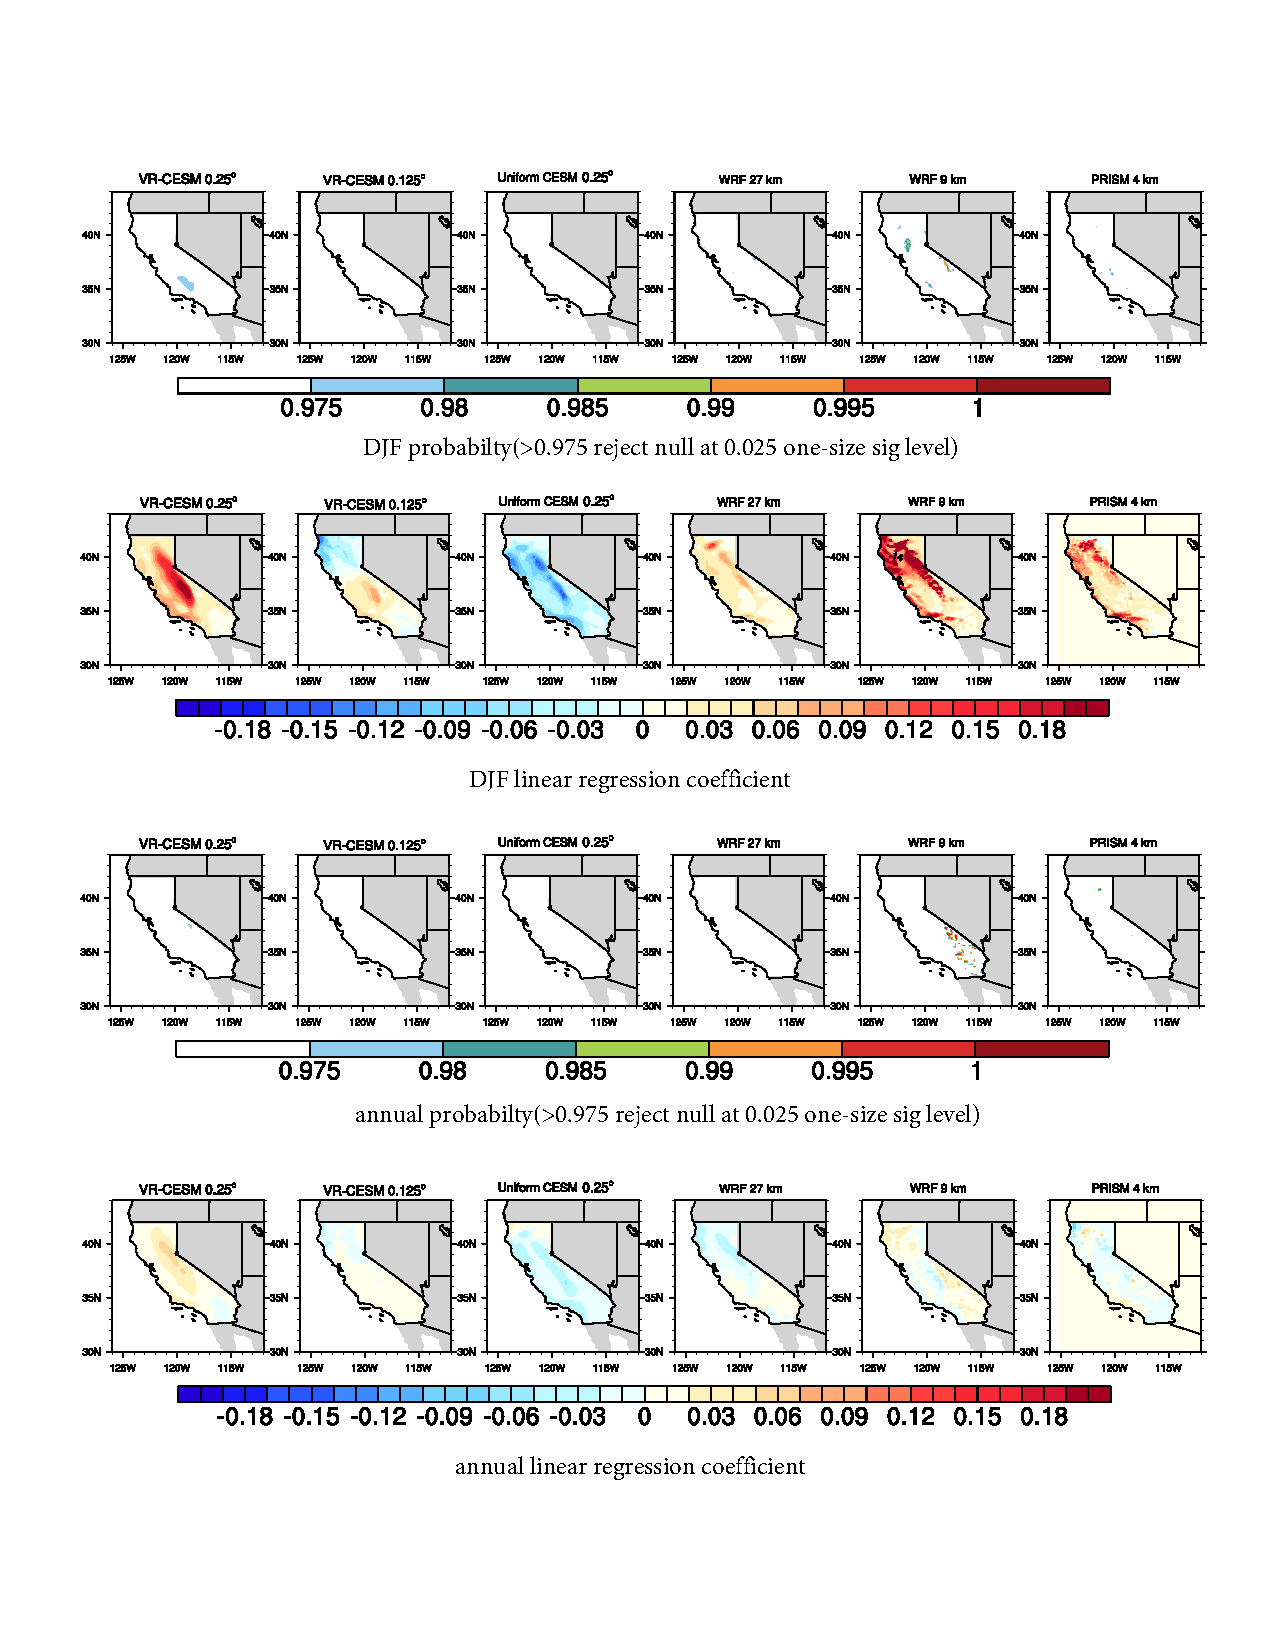
\includegraphics[width=6in]{supplement/Ttest_precipitation_timeTrend_over_1980-2005.pdf}
\caption{Results of Student's t-test for a statistically significant linear time trend of annual and DJF precipitation over 1980-2005 of models and PRISM.}
\end{center}
\end{figure}

\begin{figure}
\begin{center}
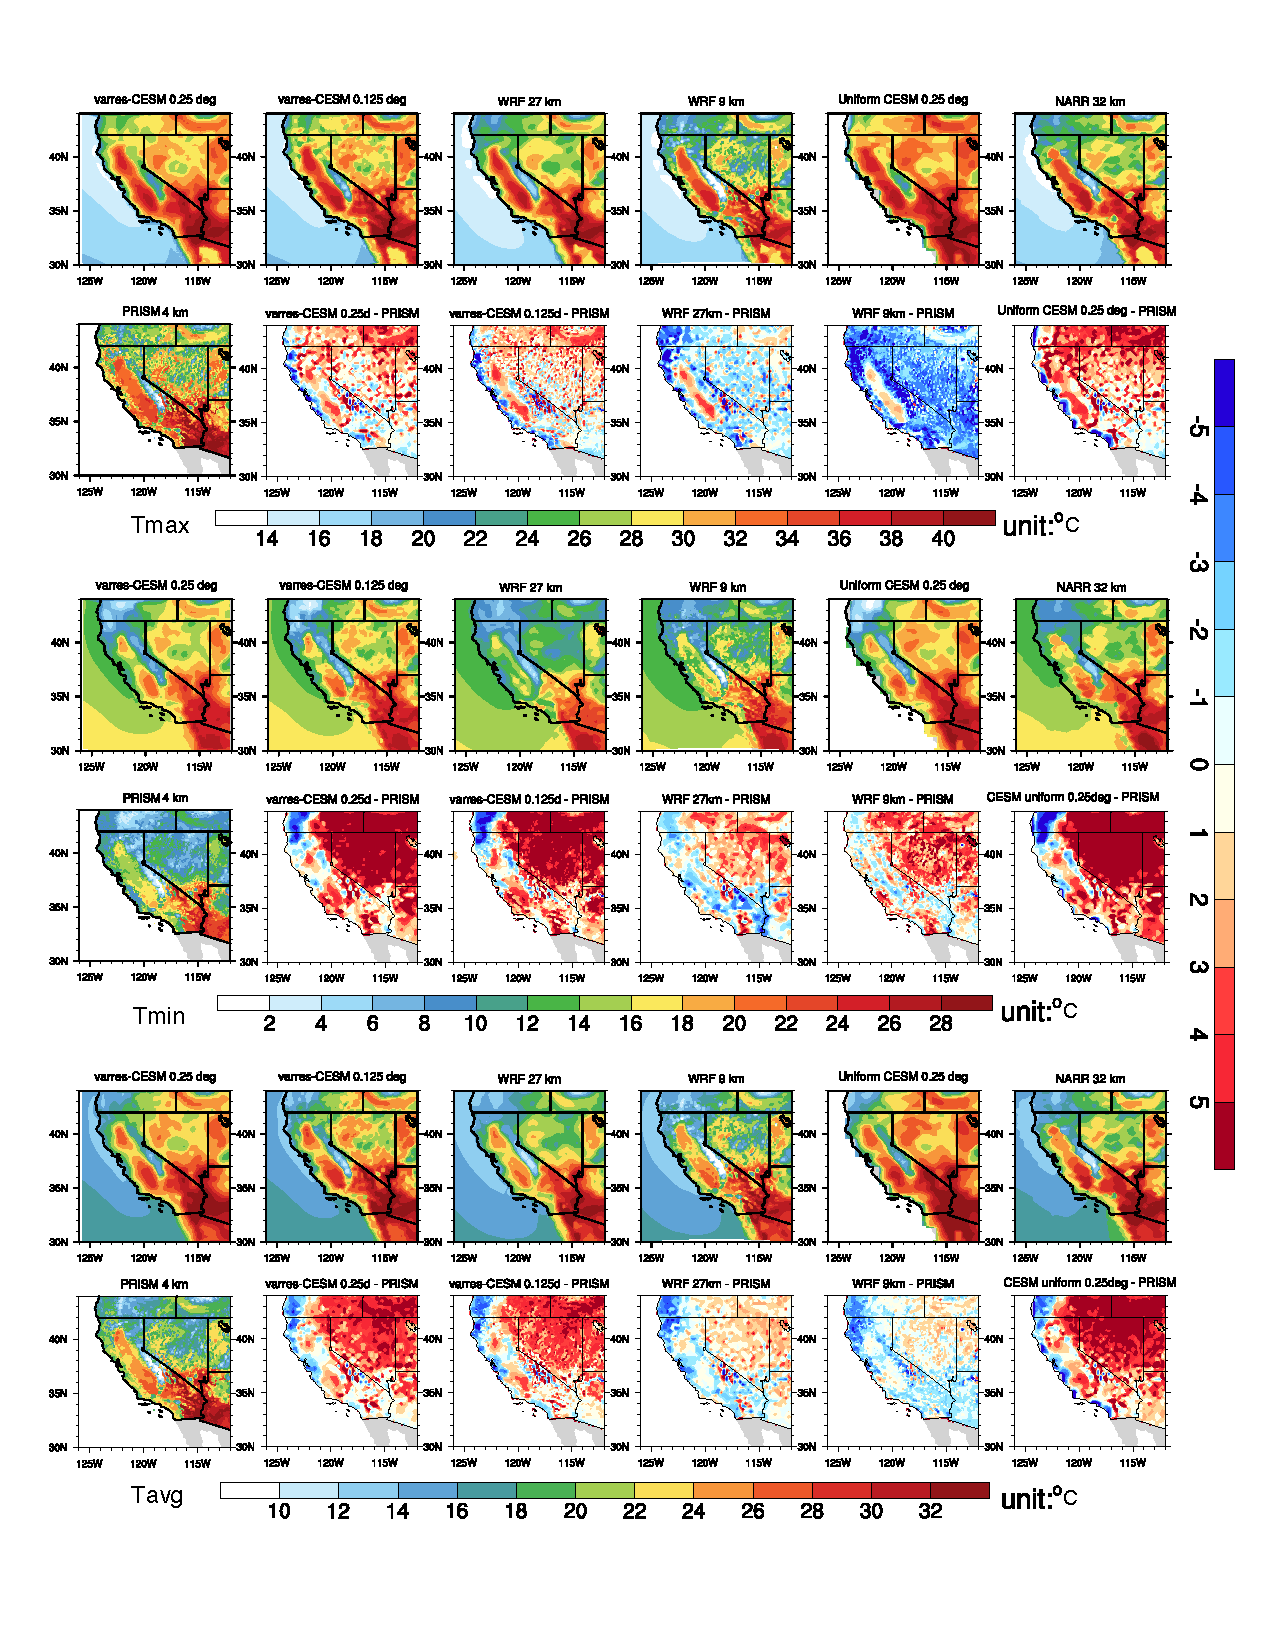
\includegraphics[width=6in]{supplement/t2_JJA_with_uniform_CESM.pdf}
\caption{Same as Figure 4 for season JJA along with uniform CESM 0.25$^\circ$.}
\end{center}
\end{figure}

\begin{figure}
\begin{center}
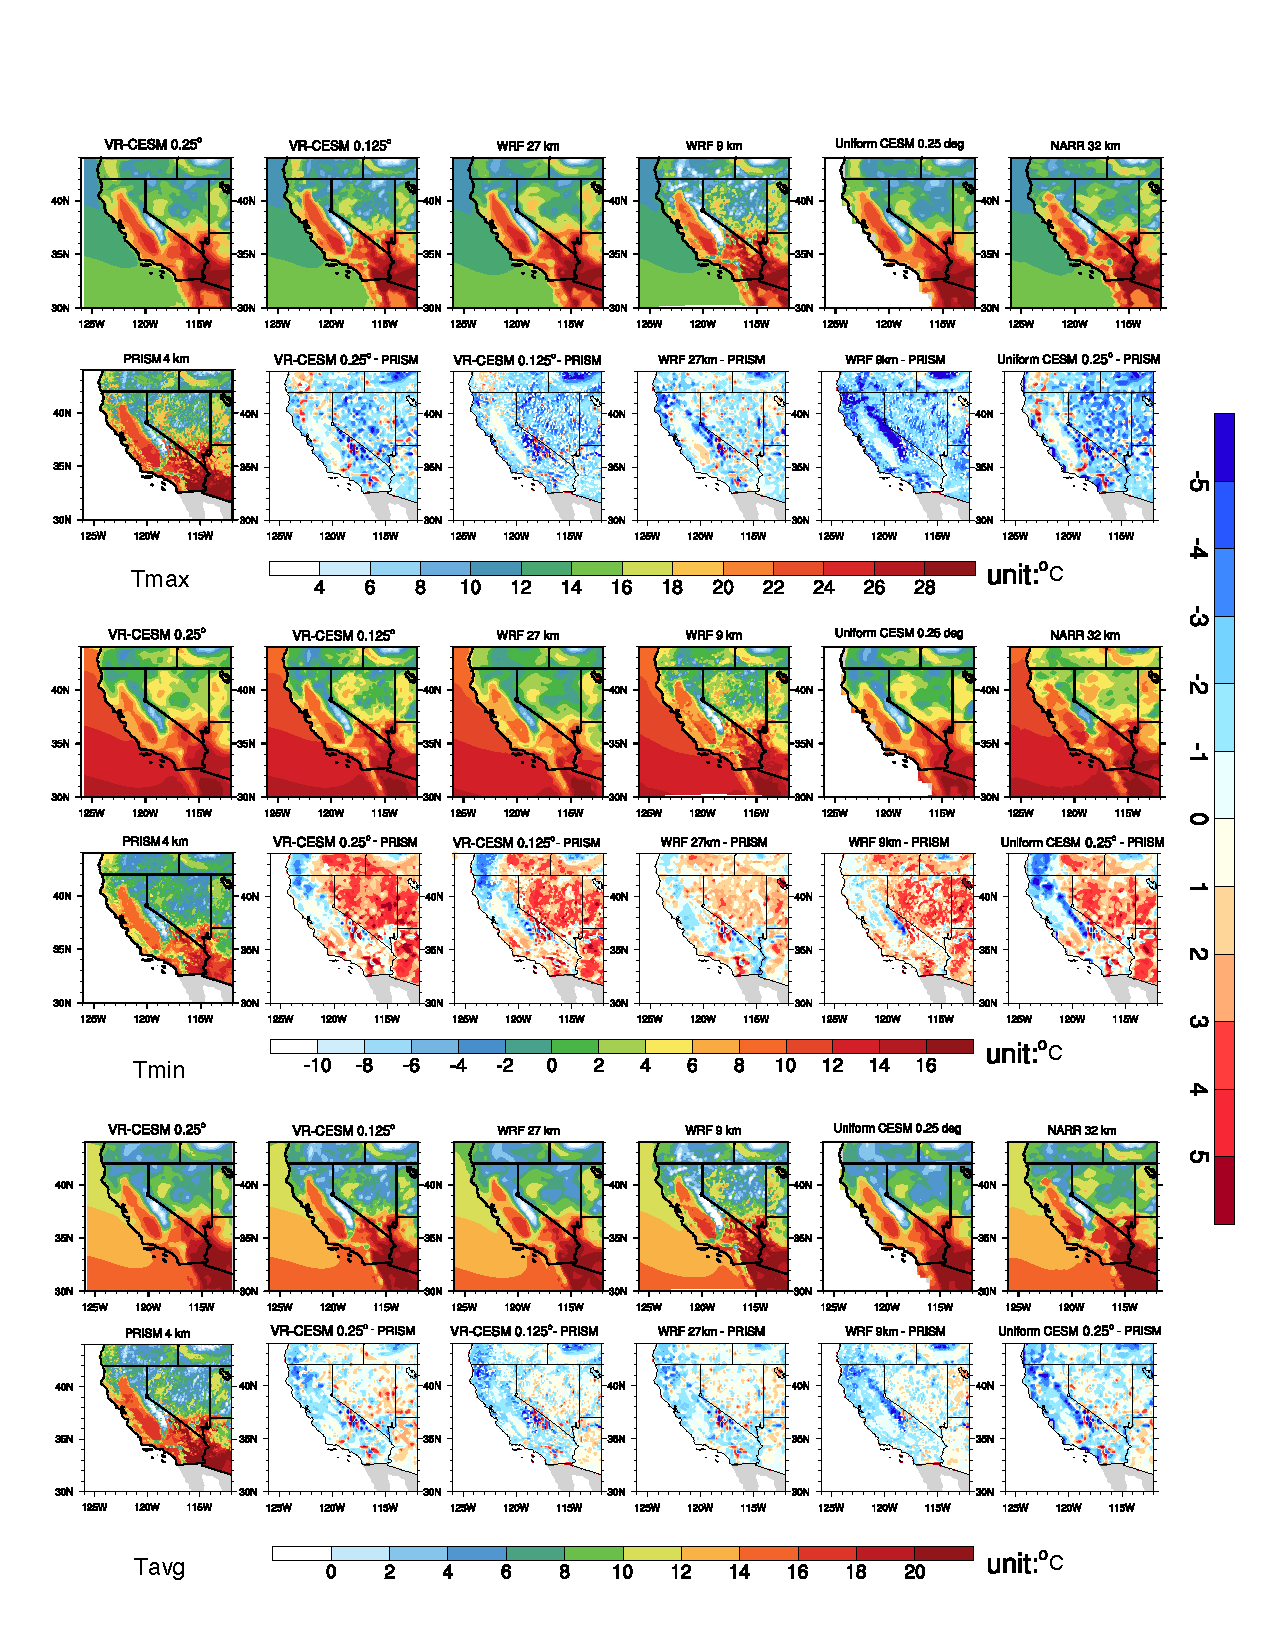
\includegraphics[width=6in]{supplement/t2_MAM.pdf}
\caption{As Figure 4 for season MAM along with uniform CESM 0.25$^\circ$.}
\end{center}
\end{figure}

\begin{figure}
\begin{center}
\includegraphics[width=6in]{supplement/t2_SON.pdf}
\caption{As Figure 4 for season SON along with uniform CESM 0.25$^\circ$.}
\end{center}
\end{figure}

\clearpage

\begin{figure}
\begin{center}
\includegraphics[width=6in]{supplement/t2_DJF.pdf}
\caption{As Figure 4 for season DJF along with uniform CESM 0.25$^\circ$.}
\end{center}
\end{figure}
%
\begin{figure}
\begin{center}
\includegraphics[width=6in]{supplement/trd_t2avg_allzones_with_uniform_CESM.pdf}
\caption{As Figure 6 but with the addition of uniform CESM 0.25$^\circ$.}
\end{center}
\end{figure}

\begin{figure}
\begin{center}
\includegraphics[width=6in]{supplement/pr_DJF_Annual_with_uniform_CESM.pdf}
\caption{As Figure 9 but with the addition of uniform CESM 0.25$^\circ$.}
\end{center}
\end{figure}

\begin{figure}
\begin{center}
\includegraphics[width=6in]{supplement/trd_pr_allzones_with_uniform_CESM.pdf}
\caption{As Figure 11 but with the addition of uniform CESM 0.25$^\circ$.}
\end{center}
\end{figure}

\begin{figure}
\begin{center}
\includegraphics[width=6in]{supplement/taylor_diagram_with_uniform_CESM.pdf}
\caption{As Figure 14 but with the addition of uniform CESM 0.25$^\circ$.}
\end{center}
\end{figure}


% ACKNOWLEDGMENTS


%\chapter{Irrigation impacts on California's climate with the variable-resolution CESM}
%

% Enter your Abstract here
\section{Abstract}

The variable-resolution capability within the Community Earth System Model (VR-CESM) is applied to understand the impact of irrigation on the regional climate of California. Irrigation is an important contributor to the regional climate of heavily irrigated regions, and within the U.S. there are few regions that are as heavily irrigated as California's Central Valley, responsible for 25$\%$ of domestic agricultural products. A flexible irrigation scheme with relatively realistic estimates of agricultural water use is employed. The impact of irrigation on mean climatology and heat extremes is investigated over the 26 year period 1980-2005 using a relatively fine grid resolution of $0.25^\circ$ ($\sim$28 km). Three simulations are performed, including an unirrigated control run and two irrigation-enabled runs, with results compared to gridded observations and weather station datasets. During the summer months (when irrigation peaks), irrigation leads to cooling of the daily maximum near-surface temperature field (Tmax) by approximately 1.1 K. Under irrigation, latent heat flux increased by $\sim$61$\%$ during the daytime as a result of increased surface evaporation; specific humidity increased by about 12$\%$; heat stress was reduced by 22$\%$ and the average soil moisture exhibited a small ($\sim$4.4$\%$) but statistically significant increase. Compared with observations, irrigation improved the frequency distribution of Tmax, and both length and frequency of hot spells were better represented with irrigation enabled. Consequently, we argue that high-resolution simulations of regional climate in CESM, particularly over heavily irrigated regions, should likely enable the irrigation parameterization to better represent local temperature statistics.


% MAIN BODY OF PAPER
\section{Introduction}

Over the past century, human activity has had a clear impact on global and regional climate, largely through indirect effects associated with increasing greenhouse gases \cite{solomon2007ipcc}, but also as a result of land cover changes, particularly deforestation, agriculture and urbanization \cite{bonan1997effects, pielke2002influence, kueppers2008seasonal}. Conversion of the natural land cover to cropland features prominently in this change, which is accompanied by modified albedo and differences in both sensible and latent heat fluxes \cite{foley2003green}. Besides affecting energy balance, land management also impacts the climate system by modifying the carbon and water cycles, which are driven in part by cropping length and irrigation strategy \cite{lobell2006biogeophysical}. The pronounced cooling effect of irrigation, especially over regions where irrigation is extensive, has been emphasized by previous studies \cite{kueppers2007irrigation, lobell2008effect}.

California is the most irrigated state in the U.S., and most of California's irrigated cropland is distributed over the Central Valley (CV), which is responsible for 25$\%$ of domestic agricultural products \cite{wilkinson2002potential}. The CV extends 600 km between its northernmost and southernmost point and is between 60-100km in width.  It features a vast agricultural industry that has adapted to an extremely dry growing season with a Mediterranean climate through the adoption of extensive irrigation practices. The USGS reported that in the year 2000, approximately 42 km$^3$ of water was used over $\sim$41,000 km$^2$ of irrigated area within California \cite{doll2002global, famiglietti2011satellites}. \cite{bonfils2007empirical} found that irrigation over CV has decreased summertime maximum temperature by $\sim$2-3 K in heavily-irrigated areas compared with nearby non-irrigated areas, based on long-term temperature records, although these impacts had a negligible effect on nighttime temperatures. Similar impacts have also been demonstrated in Nebraska's irrigated areas by \cite{mahmood2006impacts}.

However, irrigation effects are usually ignored in climate models for several reasons: irrigation usually occurs over a relatively small area ($\sim$2$\%$ of global land surface) and produces a seemingly negligible cooling effect compared to global greenhouse warming \cite{boucher2004direct}. Nonetheless, irrigation is a potentially important factor in regulating climate patterns at regions scales, where there is a growing need for accurate climate assessments and projections. Past studies have typically addressed the climatic effects of irrigation in limited-area models (LAMs) \cite{snyder2006regional, kueppers2007irrigation}, which in the context of climate modeling are typically referred to as regional climate models (RCMs). In these studies, irrigation is modeled by accounting for the amount of irrigated water needed and the area of cropland where irrigation is applied. Using a multi-model ensemble of RCM simulations, \cite{kueppers2008seasonal} found that the behavior of RCMs varied in representing effects of irrigation on regional climate, depending on each model's physics, as well as on the configuration of the irrigation parameterization.

Although global climate models (GCMs) rarely account for irrigation, it is nonetheless meaningful to understand to what extent irrigation may affect the global climate patterns \cite{sacks2009effects}. \cite{lobell2006biogeophysical} coupled the community atmosphere model (CAM) 3.0 to the community land model (CLM) 3.0 at $\sim$2-2.5$^\circ$ horizontal grid spacing to model irrigation by fixing soil moisture at saturation during the growing season in all croplands. Although this approach likely overcompensated for total added water, it produced global land surface cooling of 1.3 K, and regional cooling of up to 8 K. \cite{lo2013irrigation} used CAM 3.5 along with CLM 3.5 at $\sim$1.4$^\circ$ horizontal resolution, and argued that the increase in evapotranspiration and water vapor due to irrigation significantly impacts the atmospheric circulation in the southwestern United States by strengthening the regional hydrological cycle.

The aforementioned studies either used RCMs or coarse-resolution GCMs, along with different irrigation parameterizations. In order to model regional climate over the CV, relatively fine horizontal resolution is needed to more accurately represent microclimates, land-use, small-scale dynamical features and corresponding interactions \cite{leung2003regional, rauscher2010resolution}. In this paper, we use the recently developed variable-resolution option in Community Earth System Model (VR-CESM) to study the impact of irrigation on regional climate over the CV, that features a more flexible irrigation scheme with relatively realistic estimates of regional agricultural water use (as will be described in Section 2). Variable-resolution GCMs (VRGCMs) such as VR-CESM use a relatively coarse global model with enhanced resolution over a specific region \cite{staniforth1978variable, fox1997finite}. 


Compared with RCMs, a key advantage of VRGCMs is that they use a single, unified modeling framework, rather than a separate GCM and RCM with potentially inconsistent dynamics and physics parameterizations and lack of two-way interactions at the nest boundary \cite{laprise2008challenging}. When compared to uniform-resolution global models, VRGCMs provide a cost-effective approach for reaching high resolutions over a region of interest -- the regional simulations in this study at 0.25$^\circ$ ($\sim$28 km) resolution represent a reduction in required computation of approximately 10 times over a global uniform simulation with resolution of 0.25$^\circ$. VR-CESM has been demonstrated to be effective for regional climate studies and applications at a reduced computational cost compared to uniform GCMs \cite{zarzycki2015effects, rhoades2015characterizing, huang2016evaluation}. In particular, this study is one of the first to use variable resolution for assessing the impact of a physical parameterization at high-resolution in a global Earth-system model. The central hypothesis of this paper is that irrigation in the CV of California is an important contributor to the region's surface energy budget and must be accounted for in order to properly simulate temperature statistics, tested by a control (non-irrigated) and two irrigated 26-year simulations in VR-CESM.

This work builds on a number of previous modeling studies that have explored the importance of irrigation in controlling the climate over the CV region in the following ways: (1) it employs relatively high resolution ($\sim$28 km) covering the western U.S. over long-term period  (from year 1980-01-01 to 2005-12-31); (2) it uses a more realistic irrigation parameterization embedded in CLM 4.0 and coupled in CESM 1.2.0 rather than experimentally fixed irrigated water, as in many previous studies (\textit{i.e.} \cite{lobell2006biogeophysical, lo2013irrigation}); (3) it uses a variable-resolution global climate model (rather than the low-resolution global or limited area models forced by reanalysis dataset or GCM output that have been previously used); and (4) it explores a more comprehensive array of impacts of irrigation on the regional climate, focusing on temperature statistics, including extreme heat episodes.  We conclude that the irrigation parameterization in CESM is effective at addressing a bias in daily maximum temperatures and heatwave statistics in California's CV, and is necessary in order to accurately capture temperature statistics in heavily irrigated regions at high model resolution.

This paper is organized as follows: Section 2 describes the model setup, employed datasets and methodology. In section 3, simulation results are provided and analyzed. Key results are summarized along with further discussion in section 4.

\section{Model setup and reference datasets}

\subsection{Irrigation parameterization}

As a state-of-the-art Earth modeling framework, CESM 1.2.0 consists of coupled atmospheric, oceanic, land and sea ice models \cite{CAM5Tech, hurrell2013community}. In this study, CAM version 5 (CAM5) \cite{CAM5Tech} and CLM version 4.0 \cite{CLM40Tech} are used.  Global sea-surface temperatures are prescribed in accordance with the Atmospheric Model Intercomparison Project (AMIP) protocol \cite{Gates1992}.  The finest horizontal resolution of our grid is $\sim$28 km covering the western U.S., with a quasi-uniform 1$^\circ$ mesh over the remainder of the globe (see Figure \ref{fig:Figure 1}). Considering the relatively flat topography (less than 100 m) over most of CV, the $\sim$28 km grid resolution satisfies our need for modeling irrigation effects. In particular, simulations at 0.125$^\circ$ ($\sim$14 km) conducted in \cite{huang2016evaluation} did not show a statistically significant change in temperature statistics over California.  In our study, as in \cite{zarzycki2015effects}, general circulation patterns (e.g., wind, pressure and precipitation) do not exhibit apparent artifacts in the variable-resolution transition region. A detailed description of the techniques of VR-CESM employed in this paper can be found in \cite{rhoades2015characterizing}. Here, our model description focuses on the irrigation scheme within CLM 4.0.

\begin{figure}
\begin{center}
\includegraphics[width=6in]{gridmesh.pdf}
\caption{(a) The approximate grid spacing used for the VR-CESM 0.25$^\circ$ mesh. (b) A depiction of the transition from the global $1^\circ$ resolution mesh through two layers of refinement to $0.25^\circ$.}
\label{fig:Figure 1}
\end{center}
\end{figure}

The fractional land-use data used for computing cropland (independent of specific type) that is equipped for irrigation within each grid cell is from \cite{siebert2005development} for the year 2000, and is fixed over the simulation period (see Figure \ref{fig:Figure 2}). This assumption is reasonable since irrigated area has been largely unchanged in California since year 1980 \cite{bonfils2007empirical}. 

\begin{figure}
\begin{center}
\includegraphics[width=6in]{irrigatedArea.pdf}
\caption{The percent of irrigated cropland at each grid cell.  The black line delineates the boundary of the CV region.}
\label{fig:Figure 2}
\end{center}
\end{figure}

The need for daily irrigation is determined at 6 AM local time by computing the deficit between the current soil moisture content and a target soil moisture content.  Note that this calculation does not account for the infiltration rate of the soil. If positive, the difference is then added to the ground surface at a constant rate over the following four hours, bypassing canopy interception. By default, CLM simulates ten soil layers, with a total depth of 3.4 m \cite{CLM40Tech}. The target soil moisture content in each soil layer $i$ ($w_{target, i}$, in kg/m$^2$) is a weighted average of (a) the minimum soil moisture content that results in no water stress (w$_{o,i}$, kg/m$^2$) and (b) the soil moisture content at saturation ($w_{sat,i}$, kg/m$^2$), in accordance with

\begin{align} \label{eq:TargetSoilMoisture}
w_{target,i} = (1-{\alpha})*w_{o,i} + {\alpha}*w_{sat,i}
\end{align} The default value of the irrigation weight factor $\alpha$ is 0.7, which was determined empirically to give global, annual irrigation amounts that approximately match observed gross irrigation water use around the year 2000 \cite{shiklomanov2000appraisal}. This parameterization is designed to approximate human behavior -- that is, enough water is added so as to avoid water stress in crops, but not so much that the soil is completely saturated. More details about the irrigation model can be found in the online technical description \cite{irrigationTechnicCLM}.

\subsection{Simulations}

In order to understand the impacts on the local climate triggered by irrigation over the CV, we have conducted a control run (NRG) without irrigation and two irrigation-enabled runs, referred to as IRG and IRG(0.5) respectively. The IRG run uses the default irrigation weight factor ($\alpha = 0.7$).  This value was adjusted to 0.5 in the irrigated IRG(0.5) run so as to determine the impact of changes in total irrigation water. Simulations were performed over the period 1979-01-02 to 2005-12-31 (UTC).  For purposes of analysis, 1979 was discarded as a spin-up period to allow adequate time for the land and atmosphere to equilibrate.  Initial soil moisture conditions are specified from the output of long-term simulations so as to ensure the groundwater aquifer was initially in near-equilibrium with the local climatology. The 26-year time period was chosen to provide an adequate sampling of annual variability within computational constraints. A land cover dataset at 3 min ($\sim$10 km) grid resolution for year 2000 was used as it provided a realistic fraction of irrigated cropland in each grid cell over the CV when interpolated onto the 28 km grid (see Figure 2). 

Irrigation water applied in the IRG simulation was $\sim$2.84 mm/day in JJA when averaged over the CV, which equates to 31.7 km$^3$ total water. Given that no reliable and comprehensive dataset on cropland utilization or fallowing is available, and that information on local irrigation practices is even harder to come by, it was determined that there was no precise and publicly available numbers for the irrigation area and total utilized irrigation water over the CV. However, as mentioned earlier, in the year 2000 the USGS reported that approximately 42 km$^3$ of water was used over approximately 41,000 km$^2$ of irrigated area in California. Based on the fraction of cropland equipped for irrigation in the year 2000 obtained from \cite{siebert2005development}, we arrived at an estimate of CV irrigated area of about 33,190 km$^2$, which is about 81$\%$ of California's total irrigated area.  Assuming between half to two thirds of the 42 km$^3$ of water was employed over the CV during JJA (excluding certain water amount for late spring and early fall), that resolves to about 21 to 28 km$^3$, or 0.66 to 0.88 times the amount applied in IRG ($\sim32 \mbox{km}^3$). This suggests that the water use imposed by this irrigation scheme is relatively realistic.


\section{Methodology}

In the CV, irrigation peaks during the summer growing season \cite{salas2006estimating} in response to California's dry Mediterranean summers (with a precipitation rate of about 0.13 mm/day averaged over year 1980-2005). Our simulations accurately reproduce this observation, as most irrigated water is added during summer (see Figure 1 in the supplement document). To study the  climatological impacts of irrigation, we focus primarily on changes in June, July and August (JJA) near-surface (2 m) temperatures including daily maximum, minimum and average temperatures (Tmax, Tmin and Tavg), and the associated mechanisms driving the relative changes. 

To determine how irrigation affects heat extremes within the CV, we calculated hot spell length, hot spell frequency, and mean Tmax over the hot spells, based on the JJA daily Tmax over the 1980-2005 period. For our purposes, a hot spell is present in a given grid cell when five or more consecutive days with Tmax exceeds 38$^\circ$C. This threshold value approximately corresponds to the 90th percentile of all daily Tmax values within the CV. \textit{Hot spell length} is defined as the average duration (in days) for all  hot spells over the 26 year period, \textit{hot spell frequency} is defined as the average number of hot spells per year, and \textit{mean hot spell Tmax} is defined as the average Tmax over all the hot spell days. When analyzing hot spells, declustering is employed following the strategy of \cite{ferro2003inference} to ensure hot spells are serially independent.  This functionality is implemented in the R package \texttt{extRemes} \cite{gilleland2011new}.

To restrict the analysis to the CV, the variables of interest have been masked and/or averaged within the area defined by the bounded region as sketchily depicted in Figure \ref{fig:Figure 2}, which contains 155 grid points. To quantify model performance against reference datasets, the root-mean-square deviation (RMSD) and mean signed difference (MSD) are used, and spatial correlation (Corr) is assessed by computing sample linear cross-correlations at lag 0 after converting a two-dimensional dataset to a one-dimensional array. Mathematically, RMSD and MSD are written as, 

\begin{align}
RMSD &= \sqrt{\frac{1}{N} \sum_{i=1}^{N} (v_i - \hat{v}_i)^2}  & MSD &= \frac{1}{N} \sum_{i=1}^{N} (v_i - \hat{v}_i) 
\end{align} where $v_i$ and $\hat{v}_i$ are values from the simulation output and reference dataset respectively; $i$ is the grid-point index and N is the total number of grid points over specific regions.

Throughout the remainder of this paper, Student's t-test has been used to test the equality of the means of two datasets. This is employed for the seasonally-averaged data at each grid point and for spatially averaged data over CV. F-test is applied to test whether the sample variances are equal. These tests are used here when the sample population can be adequately described by a normal distribution, where normality is assessed under the Anderson-Darling test. All these tests are evaluated at the $\alpha = 0.05$ significance level. 

\subsection{Reference datasets}

For comparison, we employ two high-quality gridded observational datasets (UW and PRISM) and selected weather station data (NCDC) to evaluate our simulation output. The detailed descriptions of these reference datasets are as follows.

\paragraph{UW} The UW daily gridded meteorological data is obtained from the Surface Water Modeling group at the University of Washington \cite{maurer2002long, hamlet2005production}. The dataset is provided at 0.125$^\circ$ horizontal resolution covering the period from year 1949 to 2010 with daily time frequency for Tmax and Tmin in the aspect of temperature, which are used in this study.

\paragraph{PRISM} The Parameter-elevation Regressions on Independent Slopes Model (PRISM) \cite{daly2008physiographically} gridded dataset at 4 km resolution is also employed in this study.  This model ingests point measurements and applies a weighted regression scheme that accounts for key factors affecting the local climatology. PRISM is the United States Department of Agriculture's official climatological dataset. Monthly climatological variables are available for year 1895 through 2015 and daily data for year 1981 to 2015 from the PRISM Climate Group \cite{prismSource}. This study makes use of monthly Tmax, Tmin, Tavg, and daily Tmax.

\paragraph{NCDC} Weather station measurements over the CV are obtained from the Global Historical Climate Network (GHCN) and provided by NOAA/NCDC \cite{menne2012overview}. Weather stations within the study region were chosen from all stations with at least 90$\%$ observations of Tmax over all JJA days from 1981 to 2005.  A subset of 11 stations were then chosen to provide roughly even spatial coverage of the CV.

\section{Results}

The average JJA Tmin, Tavg and Tmax over the 1980-2005 period from all simulations and gridded datasets are depicted in Figure \ref{fig:Figure 3}. Relative to the gridded datasets, NRG has a prominent overestimation of Tmax, with MSD values of $\sim$0.75 K and RMSD values of $\sim$1.7 K (see Table \ref{tab:table1}). The cooling effect caused by irrigation is clear in all temperature fields when comparing NRG and IRG results, with all fields exhibiting significant differences over parts of the CV (as hatched in Figure 3). Notably, no statistically significant difference in temperature arises from reducing the irrigation factor from 0.7 to 0.5. Although the IRG run shows a slight cold bias with an MSD around -0.36 K (which is reduced in IRG(0.5) to around -0.2 K), this effect is limited to the base of the Sierra Nevada and the San Francisco Bay Delta region.

\begin{figure}
\begin{center}
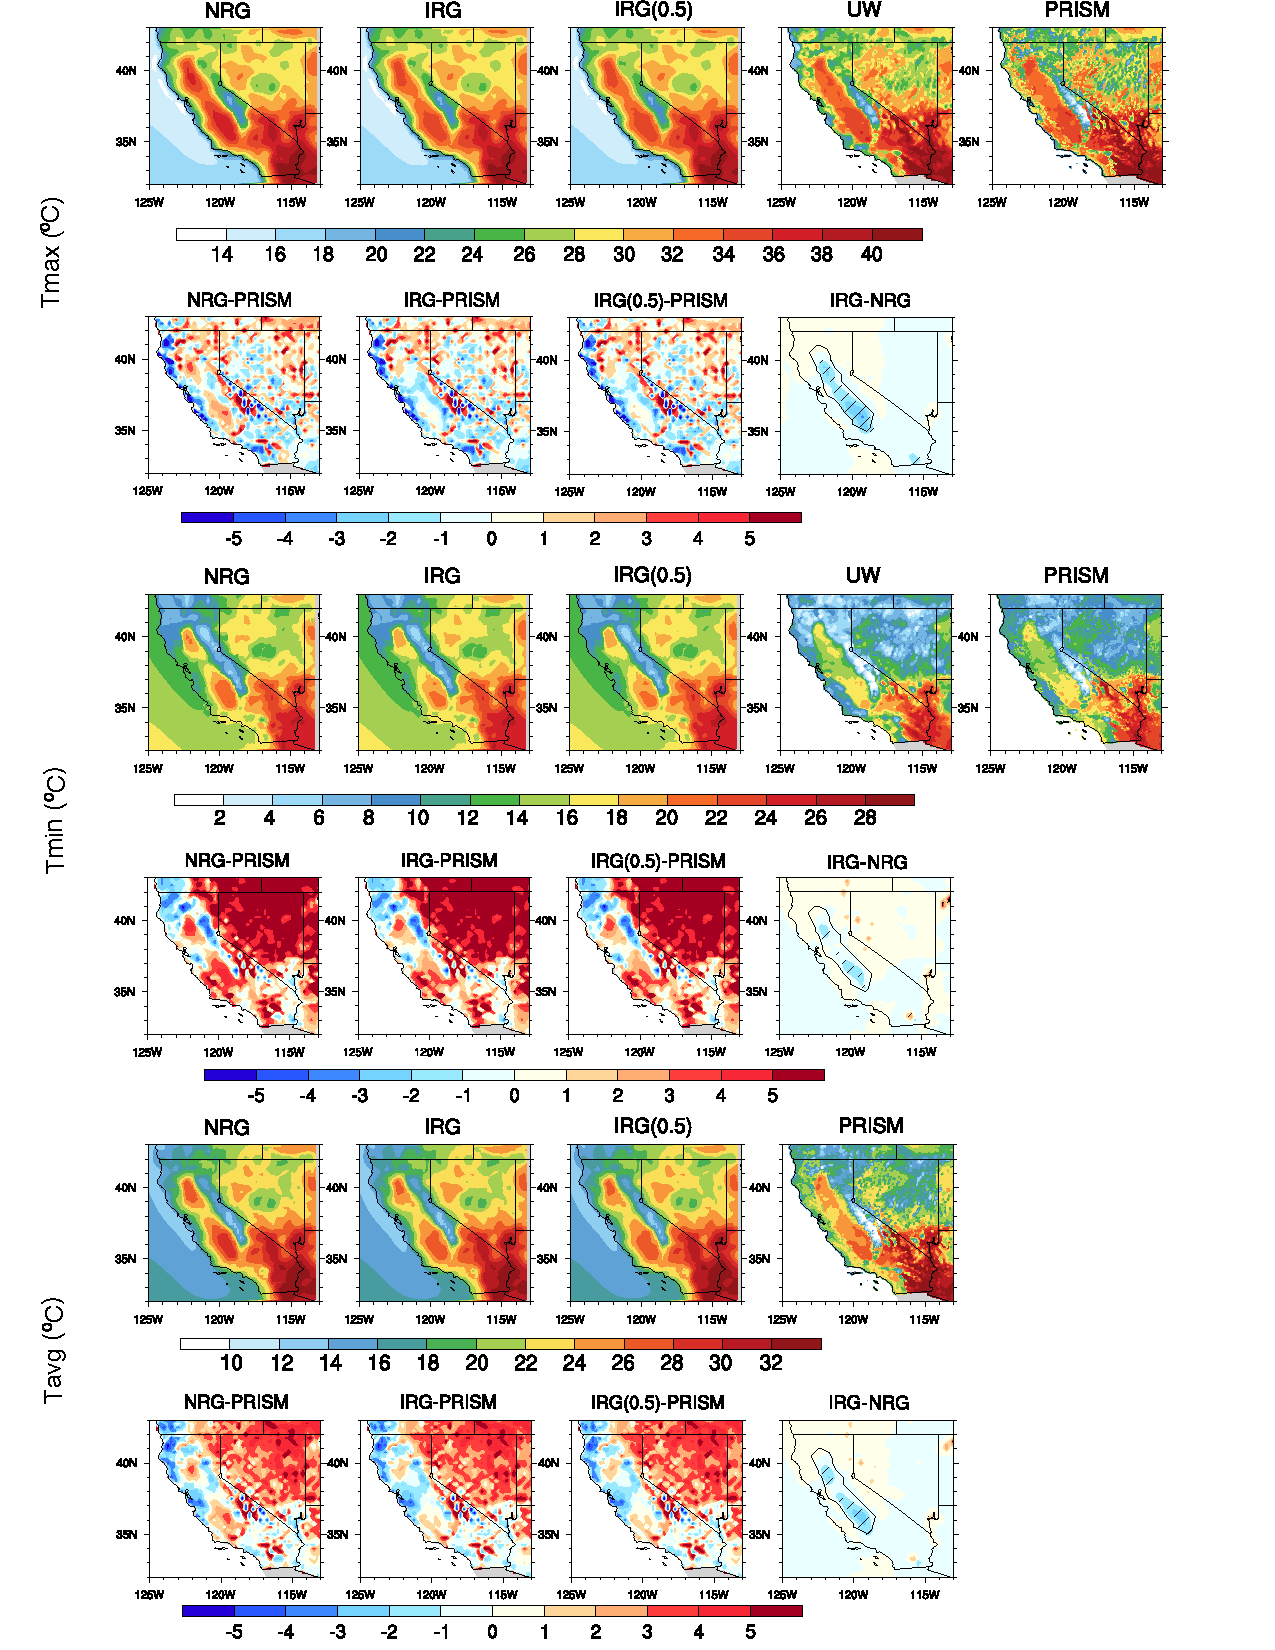
\includegraphics[width=6in]{irrig_2dplot.pdf}
\caption{Average JJA Tmax, Tmin and Tavg over year 1980-2005 for models and observations ($^\circ$C). Hatching denotes statistically significant differences between NRG and IRG.}
\label{fig:Figure 3}
\end{center}
\end{figure}

%%%%%Table 1%%%%%%%%%%%%
\begin{table}
\begin{center}
\caption{RMSD ($^\circ$C), MSD ($^\circ$C) (left column minus top row) and Corr of Tmax, Tmin and Tavg between models and gridded observations over the CV in JJA (1980-2005).} \label{tab:table1}

\begin{tabular*}{6in}{l @{\extracolsep{\fill}}cccccccccccc}
\hline \textbf{JJA Tmax} & UW  & PRISM & NRG\\
\hline $    $ & RMSD $\ $ MSD $\ $ Corr & RMSD $\ $ MSD $\ $ Corr & RMSD $\ $ MSD $\ $ Corr \\
\hline \textbf{NRG} & 1.685 $\ $ 0.749 $\ $ 0.857 & 1.689 $\ $ 0.751 $\ $ 0.856 \\
\textbf{IRG} & 1.511 $\ $ -0.357 $\ $ 0.816 & 1.422 $\ $ -0.355 $\ $ 0.841 & 1.378 $\ $ -1.105 $\ $ 0.973 \\
\textbf{IRG(0.5)} & 1.467 $\ $ -0.205 $\ $ 0.821 & 1.383 $\ $ -0.203 $\ $ 0.843 & 1.251 $\ $ -0.953 $\ $ 0.975 \\
\hline
\end{tabular*}

\begin{tabular*}{6in}{l @{\extracolsep{\fill}}ccccccccc}
\hline \textbf{JJA Tmin} & UW  & PRISM & NRG\\
\hline $    $ & RMSD $\ $ MSD $\ $ Corr & RMSD $\ $ MSD $\ $ Corr & RMSD $\ $ MSD $\ $ Corr \\
\hline \textbf{NRG} & 2.929 $\ $ 2.117 $\ $ 0.799 & 2.759 $\ $ 1.596 $\ $ 0.763 \\
\textbf{IRG} & 2.505 $\ $ 1.694 $\ $ 0.797 & 2.272 $\ $ 1.173 $\ $ 0.774 & 0.659 $\ $ -0.423 $\ $ 0.993 \\
\textbf{IRG(0.5)} & 2.536 $\ $ 1.730 $\ $ 0.797 & 2.306 $\ $ 1.209 $\ $ 0.773 & 0.625 $\ $ -0.387 $\ $ 0.993 \\
\hline
\end{tabular*}

\begin{tabular*}{6in}{l @{\extracolsep{\fill}}cccccccccccc}
\hline \textbf{JJA Tavg} & PRISM & NRG\\
\hline $    $ & RMSD $\ $ MSD $\ $ Corr & RMSD $\ $ MSD $\ $ Corr \\
\hline \textbf{NRG} & 1.746 $\ $ 0.478 $\ $ 0.851 \\
\textbf{IRG} & 1.340 $\ $ -0.309 $\ $ 0.862 & 1.066 $\ $ -0.786 $\ $ 0.983 \\
\textbf{IRG(0.5)} & 1.318 $\ $ -0.215 $\ $ 0.863 & 0.992 $\ $ -0.692 $\ $ 0.984 \\
\hline
\end{tabular*}

\end{center}
\end{table}

%%%%%%%%%%%%%

Compared with NRG, the RMSD of Tmax for IRG(0.5) is only reduced by about 20$\%$ against PRISM, which appears to be due to the offset effects caused by the non-irrigated grid cells around our study region's boundary. Although Tmin was also reduced by about 0.5 K in IRG over the irrigated area, all three runs still exhibit a warm bias in this field relative to the reference. The net result is that Tavg is overestimated in NRG over the CV, except in regions influenced by the Delta sea breeze, whereas IRG produced a slight cool bias in Tavg after alleviating the overestimation of Tmax in the northern and southern reaches of the CV. The correlation coefficients between simulations and reference datasets are about 0.76 to 0.86, indicating that VR-CESM can capture the overall spatial distributions of temperature. Although NRG and IRG are highly correlated with each other ($>$0.95), this simply implies that the spatial pattern of IRG is quite similar to NRG under spatially uniform cooling. Over non-irrigated areas, the results are essentially identical among all runs, suggesting that temperature modulation is largely a local phenomenon.

As mentioned earlier, the differences {in temperature} between the IRG and IRG(0.5) simulations were not statistically significant, and were much smaller than the differences between IRG and NRG. Therefore, the intrinsic variability (even with some differences in irrigation water amounts) is small for VR-CESM relative to the effect of irrigation. This further testifies that the statistically significant differences between IRG and NRG are due to enabled irrigation instead of random variation.

%The overall performance of VR-CESM in modeling regional climate is out of the scope of this study, but has been extensively discussed in \cite{huang2016evaluation}.

Key variables associated with the irrigation model have been tabulated in Table \ref{tab:table2}. Tmax, latent heat flux, precipitation and soil moisture are further illustrated in Figure \ref{fig:Figure 4}. With the relative scarcity of natural precipitation in summer season ($\sim$0.1 mm/day), there is a $\sim$61\% increase in latent heat flux after adding $\sim$2.84 mm/day irrigated water for IRG over the hot and dry summer period. The main contribution to latent heat flux increase from NRG to IRG is due to ground evaporation (which is about 2.5 times larger), as vegetation evapotranspiration did not differ significantly between NRG ($\sim$1.1 mm/day) and IRG ($\sim$1.25 mm/day). Therefore, cooling of Tmax is largely due to increased latent heat flux during the daytime caused by evaporation from the surface.

%%%%%%%Table 2%%%%%%%%%%%%%%%%
\begin{table}
\begin{center}
\caption{Key variables associated with irrigation within the CV in JJA (1980-2005).} \label{tab:table2}
\begin{tabular*}{7.5in}{l @{\extracolsep{\fill}}cccccccccccc}
\hline & Irrigated & Latent & Sensible & Ground & Surface & Soil & Precipitation & 2m specific \\ 
& water & heat flux & heat flux & evaporation & runoff & moisture & & humidity \\ 
& (mm/day) & (W/m$^2$) & (W/m$^2$) & (mm/day) & (mm/day) & (kg/m$^2$) & (mm/day) & (g/kg) \\ 
\hline \textbf{NRG} & 0.000 & 38.832 & 120.458 & 0.257 & 0.016 & 114.114 & 0.101 & 6.989 \\  
\textbf{IRG} & 2.838 & 62.574 & 104.752 & 0.907 & 1.610 & 119.158 & 0.119 & 7.852 \\ 
\textbf{IRG(0.5)} & 1.272 & 61.695 & 105.730 & 0.892 & 0.236 & 117.550 & 0.118 & 7.782 \\ 
\hline
\end{tabular*}
\end{center}
\end{table}
%%%%%%%%%%%%%%%%

\begin{figure}
\begin{center}
\includegraphics[width=6in]{irrig_boxplot.pdf}
\caption{Box plots for JJA averaged  (a) Tmax, (b) Latent heat flux, (c) Precipitation, and (d) Soil moisture.  From top to bottom, horizontal lines represent maximum value, third quartile, median, first quartile and minimum value, respectively.} 
\label{fig:Figure 4}
\end{center}
\end{figure}
%%%%%%%%%%%%%%

With irrigation enabled, the specific humidity increased by about 12$\%$ due to increased evaporation, and sensible heat flux decreased by 13\% with lower surface temperatures and a shift of sensible to latent heat flux. The soil moisture averaged over all surface and subsurface soil layers showed a statistically significant increase ($\sim4.4\%$) under irrigation. Since variability of the soil moisture is smaller at lower levels compared to upper levels, even a 4.4$\%$ change in the total column average was significant.  The change in soil moisture was largest near the surface, with soil water in the topmost five soil layers increased by more than 10$\%$ (reaching $\sim52\%$ at the first thin layer).


Notably, the small difference in column soil moisture (averaged over all the ten soil layers) between IRG and IRG(0.5) (equal to about 1.4$\%$, but still significant at the 95\% level) suggests that irrigated water does not effectively infiltrate into lower soil layers, given that the irrigated water applied in IRG is more than two times that of IRG(0.5). The soil water between IRG and IRG(0.5) is significantly different at the ground surface ($\sim5\%$ difference) and in the bottom layers ($\sim1\%$ difference), but not at the near-surface and throughout the middle levels. In fact, most of the additional water ($\sim$1.57 mm/day) from IRG(0.5) to IRG directly led to surface runoff (parameterized by removing surface water after infiltration into the soil at $\sim$0.24 mm/day for IRG(0.5) and $\sim$1.6 mm/day for IRG). Since irrigation water use in the IRG simulations is comparable to observations, this suggests that ineffective infiltration could be driving substantial water waste in the CV.


Based on the JJA-averaged values of each year over the 26-year period, box-and-whisker diagrams for four selected variables are given in Figure \ref{fig:Figure 4}. With irrigation, both the average magnitude and annual variability of Tmax (around 0.9$^\circ$C) are closer to observations. Compared to NRG, the range of Tmax for irrigation runs reduced to $\sim$3$^\circ$C from $\sim$4.5$^\circ$C with a more concentrated distribution, suggesting that there may be some indication of irrigation having a modulating effect on temperature variability (although the differences of variances are not statistically significant). The mean latent heat flux almost doubles when irrigation in enabled, however the variance of the distribution (with inter-annual {standard deviation} of $\sim$2.7 $W/m^2$ for IRG and $\sim$3.3 $W/m^2$ for IRG(0.5)) did not substantially differ from NRG (with inter-annual {standard deviation} of $\sim$3.7 $W/m^2$). 

Average precipitation also did not significantly change among these three runs (under the Mann-Whitney-Wilcoxon test at 0.05 level together with the observations of $\sim$0.13 mm/day for UW and $\sim$0.14 mm/day for PRISM), however adding irrigation tended to widen the range of precipitation intensity (significantly different, with inter-annual variability around 0.12 to 0.13 mm/day for irrigation runs, and about 0.08 mm/day for NRG). This is possibly due to enhanced local convective processes driven by irrigation modifying the depth of planetary boundary layer, lifting condensation level, and mixing layer (also found by \cite{kawase2008impact, deangelis2010evidence, qian2013modeling}).  A statistically significant increase in convective available potential energy (CAPE) over the irrigated region and part of its surrounding area was observed in our results (see Figure 3 in the supplement). The mean soil moisture significantly increased under irrigation, with the {standard deviation} of soil moisture decreasing significantly between IRG (about 1.5 $kg/m^2$) and NRG ($\sim2.2 kg/m^2$), likely simply due to modulation of soil moisture content associated with the irrigation parameterization.

As irrigation clearly led to a strong cooling effect for average Tmax over the hot summers of the CV, we further investigated the frequency distribution of Tmax (as depicted in Figure \ref{fig:Figure 5}) based on all JJA daily values at each CV grid point for all runs and reference datasets including UW, PRISM and 11 weather stations (area weighted using Voronoi diagram). Since PRISM does not provide daily data for the year 1980, we only assess the period 1981 to 2005 in this calculation. Overall, the NRG run exhibited an obvious warm bias associated with a relatively long forward tail with Tmax approaching 48$^\circ$C.  This forward tail was also absent from the NCDC weather station data, adding further evidence that it is associated with unrealistically frequent warm temperatures. However, with irrigation enabled there was much closer agreement with UW and PRISM, especially in the upper tail, although a slight cold bias remains. Examining absolute differences, the first four moments of the frequency distribution of Tmax all showed marked improvement under irrigation (Table \ref{tab:table3}). Under the Kolmogorov-Smirnov (KS) test, compared with UW and PRISM, the spatially averaged JJA Tmax over the CV for the 25 years (resulting in 25 values) was significantly different for NRG at the 90\% level, whereas the difference was not significant for IRG or IRG(0.5).

\begin{figure}
\begin{center}
\includegraphics[width=6in]{irrig_pdf.pdf}
\caption{Frequency distribution of JJA daily Tmax over the period 1981-2005 from simulations and reference datasets.}
\label{fig:Figure 5}
\end{center}
\end{figure}

%%%%%%%%Table 3%%%%%%%%%%%%%%%%%%%%%%%
\begin{table}
\begin{center}
\caption{The first four moments of the JJA Tmax frequency for models and observations over CV. Column titles refer to the Average (Avg), Variance (Var), Skewness (Skew) and Kurtosis (Kurt).} \label{tab:table3}
\begin{tabular*}{4in}{l @{\extracolsep{\fill}}cccccc}
\hline & Avg &Var & Skew & Kurt \\
\hline \textbf{NRG} & 33.535 & 25.732 & -0.445 & 0.252 \\
\textbf{IRG} & 32.374 & 21.343 & -0.505 & 0.415 \\
\textbf{IRG(0.5)} & 32.537 & 21.125 & -0.556 & 0.632 \\
\textbf{UW} & 32.745 & 22.442 & -0.717 & 0.794 \\
\textbf{PRISM} & 32.814 & 24.007 & -0.802 & 1.120 \\
\hline
\end{tabular*} \\

\begin{tabular}{p{3in}}
\small\textbf{Notes:} If skew $>0$ [skew $<0$], the distribution trails off to the right [left]. If kurtosis $> 0$ [$<0$], a sharper [flatter] peak compared to a normal distribution (leptokurtic and platykurtic, respectively) is expected.
\end{tabular}
\end{center}
\end{table}
%%%%%%%%%%%%%%

Hot spell features related with heat extremes are tabulated in Table \ref{tab:table4} for simulations and the UW dataset (results from PRISM were effectively equivalent to UW). Hot spells were too long and too frequent without irrigation, but once irrigation was enabled, number, duration and intensity were all closely matched to UW by the model (no significant differences under t-test). Notably, the cooling effect associated with irrigation led to a reduction in length and frequency of hot spells of about 20$\%$ and 30$\%$, respectively (both statistically significant at the 0.05 level). The difference in Tmax between IRG and NRG runs when averaged over hot spells, compared with the seasonal average, was approximately halved (but still significant). It appears that irrigation has less impact on the temperature of hot days, compared with average summer days.

%%%%%%%Table 4%%%%%%%%%%%%%%%
\begin{table}
\begin{center}
\caption{Hot spell features including length (days), number and mean Tmax ($^\circ$C) from simulations and UW data over the CV in JJA from 1980-2005.} \label{tab:table4}
\begin{tabular*}{4.5in}{l @{\extracolsep{\fill}}cccc}
\hline & NRG & IRG & IRG(0.5) & UW \\									
\hline \textbf{Hot spell length} & 8.810 & 7.014 & 6.483 & 6.930 \\ 
\textbf{Hot spell number} & 2.174 & 1.500 & 1.505 & 1.539 \\  
\textbf{Hot spell Tmax} &  40.340 & 39.806 & 39.887 & 39.720 \\ 
\hline
\end{tabular*} 
\end{center}
\end{table}

\clearpage
%%%%%%%%%%%%%%

Due to the important role the CV plays in agricultural industry, we have also examined the heat stress experienced by crops. As defined by \cite{teixeira2013global}, heat stress can be quantified by the number of hours per day exceeding 35$^\circ$C. In our study, heat stress was assessed for days from June 1st to September 30th (JJAS) for NRG and IRG runs. Given only daily outputs of Tmin and Tmax (as opposed to hourly temperature values), heat stress was obtained using a cosine fit to approximate hourly temperatures. This approach was validated by comparing the number of hours exceeding 35$^\circ$C from one year of simulation with hourly output against the cosine approximation. Since the observed discrepancy was only about 4$\%$, the cosine approximation was subsequently applied to obtain hourly temperature exceedance over the 26-year study period in the CV. Based on the averaged hourly counts (depicted in Figure \ref{fig:Figure 6}), it was observed that both the heat stress intensity and frequency were reduced under irrigation, most obviously during mid-July to early September. The average hours per day exceeding 35$^\circ$C over the JJAS period was 2.352 for NRG and 1.838 for IRG -- a $\sim$22$\%$ decrease.

\begin{figure}
\begin{center}
\includegraphics[width=6in]{irrig_hours_T2>=35.pdf}
\caption{The number of hours larger than or equal to 35$^\circ$C per day from June 1st to September 30th averaged over 1980-2005, for NRG and IRG runs.}
\label{fig:Figure 6}
\end{center}
\end{figure}


\section{Discussion and Summary}

With irrigation employed, nighttime warming is expected to occur, leading to an increase in daily Tmin due to the increased thermal conductivity of wet soil, as found by \cite{kanamaru2008model}. However, in our irrigation-enabled runs, Tmin did not increase but instead decreased over part of the irrigated area (statistically significant, although the magnitude of this decrease was much smaller than that of Tmax). As argued by \cite{bonfils2007empirical}, our result further supports the conclusion that irrigation does not completely explain the large nighttime warming observed in California. As discussed in \cite{kueppers2008seasonal} and \cite{kanamaru2008model}, the sign of the change in Tmin associated with irrigation depends on the particular parameterization and the assessed climate model.  These differences are further associated with differences in soil properties, including soil heat capacity and conductivity, and on nighttime soil-air temperature gradient. Our study matches the findings of previous studies that irrigation generally lowers temperatures in the CV region, but with a smaller magnitude ($\sim$1.1 K) than claimed by \cite{lobell2006biogeophysical}. 


\cite{lo2013irrigation} concluded that increases in evapotranspiration and water vapor export caused by irrigation significantly impacts the atmospheric circulation in the southwestern United States, including strengthening the regional hydrological cycle.  Their study was conducted using coupled CAM 3.5 and CLM 3.5 at the grid resolution of 1.4$^\circ$. However, irrigation was accounted for in this work using an approach substantially different from the present study: namely, they prescribed a fixed soil moisture which accounted for all irrigated water (around 16.7 km$^3$/JJA) within the irrigated area -- this is in contrast with our approach which only obtained soil moisture via infiltration from applied surface water.  Unlike in \cite{lo2013irrigation}, we observed no evidence for an enhanced hydrological cycle and associated increase in water vapor transport. Namely, our simulations exhibit no significant changes at the 90$\%$ level (the same level as \cite{lo2013irrigation} used) to precipitation, low-level cloud, near-surface specific humidity and CAPE, and the moisture flux anomaly at 850 hPa over the U.S. southwest, where \cite{lo2013irrigation} found changes attributed to irrigation in the CV (see Figure 3 in the supplement). We do see that there are certain positive increases of precipitation, low-level cloud and CAPE between IRG and NRG over some regions of Nevada and Utah, but these are not present when comparing IRG(0.5) and NRG.


We have also explored the possible mechanisms by which irrigation may bring about global change, including latent heat flux, near-surface specific humidity, precipitation and global cloud cover. The quantitative impacts are quite similar to what has been obtained in \cite{sacks2009effects}, and so are not repeated here. In order to determine if irrigation changes the overall atmosphere circulation, the 500 hPa geopotential height field was examined (see Figure 2 in supplement).  We observed that the large-scale pattern was similar in all cases, although statistically significant differences did sporadically arise. Since no clear pattern was present among regions with statistically significant differences, and there is no clear physical mechanism to connect these regions with irrigated areas, we attribute these differences to insufficient ensemble size.


By decreasing the irrigation weight from 0.7 to 0.5, total irrigated water employed was nearly reduced by half. Nonetheless, the climatological impacts observed in IRG(0.5) were quite similar to IRG. To understand the climatological impacts under an extreme water deficit, we also performed a five year test run in which the irrigation weight factor was set to zero, and added half of the water that was calculated from the deficit equation described in Section 2, resulting in irrigated water being applied at 0.42 mm/day. In this case, the average latent heat flux was around 50.65 W/m$^2$, which is about 80$\%$ of the value of IRG run.  This emphasizes the non-linear dependency between irrigated water application and resultant latent heat flux: specifically, most of the extra water applied in the irrigation calculation simply resulted in surface runoff rather than an enhancement of soil moisture, suggesting that CLM performs relatively conservatively in soil moisture regulation. According to the CLM 4.0 technical report \cite{CLM40Tech}, the maximum infiltration capacity is determined from soil texture and soil moisture \cite{entekhabi1989land} and the runoff is parameterized by the simple TOPMODEL-based \cite{beven1979physically} runoff model (SIMTOP) described by \cite{niu2005simple}. In CLM 4.0, the surface and subsurface runoff are assumed to be washed into nearby rivers and then end up in ocean.  CLM 4.0 does provide a simple river routing model (RTM) which was not enabled in our simulations since it lacks the realistic control of water infiltration or groundwater replenishment present in a watershed model. To accurately address the implications of irrigation, we expect that a coupled integrated hydrological modeling system is necessary to correctly represent regional hydrological processes.



To summarize, the variable-resolution Community Earth System Model (VR-CESM) was used to simulate the impact of irrigation on the regional climate of California's Central Valley (CV), one of the most heavily irrigated and productive areas in the U.S. Within the land component model (CLM), an irrigation scheme with relatively realistic estimates of water use was employed. The cooling effect caused by irrigation was obvious in the Tmax field with a magnitude around 1.1 K (seasonally averaged over summer months), which arose from the greatly increased ($\sim$61$\%$) latent heat flux associated with daytime ground evaporation. With irrigation, both the average magnitude and annual variability of Tmax were better captured when compared with gridded observations and weather station data. Compared with Tmax, smaller differences were observed for Tmin over the irrigated area, but no statistically significant impacts from irrigation were observed over the surrounding non-irrigated area's climate. Although irrigated water did not effectively infiltrate into lower soil layers, soil moisture nonetheless exhibited a statistically significant increase (with a slight amplitude $\sim$4.4$\%$) under heavy irrigation. With irrigation enabled, an exceptional warm bias associated with a long forward tail of the frequency distribution of Tmax is alleviated, although a slight cold bias remained at higher elevations. Further, the cooling effect associated with irrigation led to a reduction in length and frequency of hot spells for about 20$\%$ and 30$\%$, closely matched to observations, and a decrease in the heat stress frequency by about 22$\%$ for cropland. This work suggests that the irrigation scheme should be enabled for regional climate studies with CLM and CESM, particularly over heavily irrigated regions.

In this study, we have argued that irrigation in the CV is an important component of the region's surface energy budget that must be parameterized in high-resolution climate models in order to properly simulate temperature statistics. The ongoing California drought (2012-present) highlights the importance of water resources to agriculture in the CV. In the absence of surface water for irrigation, groundwater reserves were depleted in order to maintain agricultural production.  However, it is widely acknowledged that in a prolonged future drought, continued groundwater pumping would not be sustainable, which would in turn lead to a reduction in applied irrigation water.  This study suggests that under these conditions, warming from climate change, which is tampered by irrigation in the CV, would be exacerbated and leads to a substantial increase in daily Tmax throughout the CV with repercussions for human health and heat stress \cite{williams2015contribution}. Consequently, we anticipate this study can be extended to better understanding the feedbacks associated with prolonged drought conditions in the U.S. Southwest.

%\section{Acknowledgments}
%
%The authors would like to thank Dr. Travis O'Brien, Dr. Richard Grotjahn and Dr. Graham E. Fogg for many useful suggestions. We would also like to thank IT support for our local UC Davis computing cluster. We acknowledge the substantial effort behind the datasets used in this study, including PRISM, UW and NCDC. The simulation data used is available by request at xyhuang@ucdavis.edu. 

We acknowledge the substantial effort behind the datasets used in this study, including PRISM, UW and NCDC. This work is supported in part by the University of California, Davis and by the Department of Energy ``Multiscale Methods for Accurate, Efficient, and Scale-Aware Models of the Earth System'' project (Award No. DE-AC02-05CH11231). Support also comes from the California Agricultural Experiment Station (project CA-D-LAW-2203-H).

\section{Supporting Information}

This supplement includes:

\begin{itemize}

\item[1)] The irrigated water of IRG run, and the precipitation for both NRG and IRG runs over each of the four seasons, averaged over the period 1980-2005. 

\item[2)] The geopotential height at 500 hPa for all the simulations averaged over JJA from 1980-2005.

\item[3)] The averaged JJA Precipitation, low-level cloud, near-surface specific humidity and convective available potential energy (CAPE) of all the simulations and their differences with t-test results for year 1980-2005 period.

\end{itemize}

%%%%figure%%%%%%

\begin{figure}
\begin{center}
\includegraphics[width=6in]{supplement/irrigated_water_and_precipitation_4seasons.pdf}
\caption{Irrigated water from IRG, and precipitation for both NRG and IRG for each of the four seasons, as averaged over the period 1980-2005.}
\end{center}
\end{figure}

\begin{figure}
\begin{center}
\includegraphics[width=6in]{supplement/geopotential_height_500hPa_JJA.pdf}
\caption{Geopotential height at 500 hPa for all simulations (averaged over JJA from 1980-2005).}
\end{center}
\end{figure}

\begin{figure}
\begin{center}
\includegraphics[width=6in]{supplement/irrig_discussion_vs_Lo2013.pdf}
\caption{Precipitation, low-level cloud, near-surface specific humidity and CAPE for all simulations and their differences with t-test results (averaged over JJA from 1980-2005).}
\end{center}
\end{figure}




















%\chapter{The changing character of twenty-first century precipitation over the western United States in the variable-resolution CESM}

% Enter your Abstract here

\section{Abstract}

The changing character of precipitation frequency and intensity in the western United States over the 21st century is investigated using an ensemble of 26-year simulations with the variable-resolution Community Earth System Model (VR-CESM) at a local grid resolution of $\sim$0.25$^\circ$.  Simulations are forced using prescribed sea-surface temperatures, sea-ice extent and greenhouse gas concentrations from the representative concentration pathway (RCP) 8.5 scenario.  VR-CESM is shown to be effective at accurately capturing the spatial patterns of the historical precipitation climatology. In the Intermountain West and Southwest U.S., we observe a statistically significant increase in mean precipitation and rainy days through mid-century, although this trend is tampered by end of century in response to a decrease in relative humidity.  In the Pacific Northwest, extreme precipitation events are observed to increase significantly as a result of increased cool season integrated vapor transport.  In particular, extreme precipitation in this region appears to increase more rapidly than would be predicted by the Clausius-Clapeyron relationship.  No clear climate signal emerges in mean precipitation or for extremes in California, where the precipitation climatology is subject to large interannual variability that is tied more closely to ENSO.  Results are discussed in the context of the existing literature on precipitation extremes in the western U.S.


% MAIN BODY OF PAPER
\section{Introduction}

There is substantial and growing interest in understanding the character of precipitation within a changing climate, motivated largely by its pronounced impacts on water availability and flood management in both human and natural systems \cite{hegerl2004detectability, kharin2007changes, scoccimarro2013heavy}.  Among past studies addressing precipitation, extremes have been a major focus, particularly drought and flood events \cite{seneviratne2012changes}.  Overall, it is widely agreed that although atmospheric water vapor concentration is increasing, the impacts of a changing climate on the character of precipitation is far more complicated.  Extreme precipitation events are particularly nuanced:  Our best projections suggest that extreme precipitation events will intensify even in regions where mean precipitation decreases \cite{tebaldi2006going, kharin2007changes}.


Future climate projections, particularly those addressing the frequency and intensity of rare events, are inevitably subject to large uncertainties.  Nonetheless, climate models have been invaluable tools for developing insight into this problem \cite{easterling2000climate}. In particular, global climate models (GCMs) have often been used to investigate changes in the mean, variability and extremes of climate, as forced with predicted greenhouse gas (GHGs) concentrations and aerosol emissions \cite{meehl2006future}. Although several past studies have investigated climate extremes at the global scale \cite{seneviratne2012changes}, studies addressing extremes at local and regional scales are less common.  It is well understood how increased GHG concentrations have contributed to the observed intensification of heavy precipitation events over the tropical ocean \cite{allan2008atmospheric} and the majority of Northern Hemisphere overland areas \cite{min2011human}, but changes are much more poorly understood at regional scales where meteorological variability is large \cite{trenberth2011changes}.  As a consequence of this variability, confidence in the assessment of regional extreme precipitation changes requires both high spatial resolution and a long integration period, both of which can make the computational cost untenable for global simulations.  This issue of insufficient regional-scale climate information has been a major outstanding problem in climate science, as stakeholders and water managers typically require fine-scale information on climate impacts in order to effectively develop adaptation and mitigation strategies.


Dynamical downscaling with regional climate models (RCMs) has been one of the few tools available to ascertain the frequency, intensity, and duration of extreme events at the needed scales.  By only simulating a limited regional domain, RCMs better capture fine-scale dynamical features with high horizontal resolution \cite{bell2004regional, frei2006future, rauscher2010resolution, wehner2013very}. Higher resolution enables more accurate simulation of precipitation extremes, which are driven by circulation patterns, cloudiness, land use, land/water contrast, snowpack and topography \cite{leung2003regional, diffenbaugh2005fine, salathe2008high, wehner2010effect}. For example, \cite{leung2003hydroclimate} showed that the higher-resolution RCMs yield more realistic precipitation patterns and produce more frequent heavy precipitation over the western U.S. (WUS), consistent with observations. \cite{diffenbaugh2005fine} studied both extreme temperature and precipitation events over the contiguous United States using a RCM configured at 25 km horizontal resolution, and demonstrated that fine-scale processes were critical for accurate assessment of local- and regional-scale climate change vulnerability. \cite{salathe2008high} found significant differences in trends for temperature and precipitation over the Pacific Northwest using a high-resolution RCM for future climate simulations.  And \cite{ashfaq2016high} observed a 7.4\% increase in precipitation from extremes over the contiguous U.S. from simulations with RegCM4 driven by CMIP5 global data.


Despite their success, RCMs also have known issues associated with inconsistency between the lateral forcing data and the driven RCM.  The menu of physical parameterizations and tuning parameters typically available to RCMs can also lead to over-tuning of the model for a particular geographic region or climatological field \cite{mcdonald2003transparent, laprise2008challenging, mesinger2013limited}.  Consequently, there has been growing interest in variable-resolution enabled GCMs (VRGCMs) to improve regional climate simulations. Unlike RCMs, which require GCM data to drive the simulation at lateral boundaries, VRGCMs use a unified model with coarse global resolution and enhanced resolution over a specific study region \cite{staniforth1978variable, fox1997finite}. VRGCMs have demonstrated competitive ability for regional climate studies at a reduced computational cost, particular when compared to uniform-resolution GCMs \cite{fox2006variable, rauscher2013exploring}.


In this paper, we utilize the recently developed variable-resolution option in the Community Earth System Model (VR-CESM).  VR-CESM is based on the CESM (and its predecessor, the Community Climate System Model (CCSM)), a family of models that have been used for decades to study the global climate \cite{neale2010description, hurrell2013community}.  The overall performance of VR-CESM for modeling regional climate in the California and Nevada is detailed in \cite{huang2016evaluation}, where it was argued that VR-CESM has competitive biases in comparison to the Weather Research and Forecasting (WRF) model (a traditional RCM) and the uniform-resolution CESM, when evaluating against high-quality observations and reanalysis. VR-CESM has been used in a number of studies to simulate fine-scale atmospheric processes  \cite{zarzycki2014using, zarzycki2015effects, rhoades2015characterizing, huang2016irrigation, rhoades2016projecting}.


This study focuses on changes in the character of precipitation over the 21st century within the WUS, as predicted from long-term ensemble runs conducted with VR-CESM with a local grid resolution of $\sim$0.25$^\circ$.  The WUS is known to be particularly vulnerable to hydrological extremes, particularly floods and droughts \cite{leung2003hydroclimate, caldwell2010california}, and hosts a variety of local features and microclimates associated with its rough and varied topography.  Simulations of the future climate are performed in accordance with the representative concentration pathway (RCP) 8.5 scenario, which describes a ``business-as-usual'' projection for GHGs \cite{riahi2011rcp}.  In this study we focus singularly on the RCP 8.5 scenario because its mid-century results are similar to a more optimistic RCP2.6 scenario end-of-century.  Simulations are further conducted in accordance with the Atmospheric Model Intercomparison Project (AMIP) protocol \cite{Gates1992}, a widely-used approach for climate model diagnosis, validation and intercomparison that imposes global sea surface temperatures (SSTs) and sea ice.  It is well-known that correctly simulating changes to the spatial pattern of SSTs in state-of-the-art coupled GCMs remains a significant challenge \cite{joseph2006enso, stevenson2012significant, jha2014sst, taschetto2014cold}.  However, by constraining atmospheric boundary conditions at the sea surface, we avoid model biases that are known to exist in the fully coupled configuration \cite{grodsky2012tropical, small2014new} but accept potential uncertainties associated with our choice of SSTs.

Changes in the character of precipitation, in terms of frequency and intensity, have been assessed in our study from recent history through the end of the 21st century.  A comprehensive set of indices for precipitation extremes have been evaluated from the ensemble simulations over the 26-year periods corresponding to historical (1980-2005), mid-century (2025-2050) and end-of-century (2075-2100). Spatial inhomogeneity in local geography and temperature are observed to result in similarly inhomogeneous impacts on the precipitation field.  Teleconnections (specifically the El Nin\~o-Southern Oscillation, ENSO) are also observed to have a pronounced impact on precipitation features.  Since only one SST dataset was used for this study, we note that our projections are conditioned on a particular future character of ENSO.  This is a potentially large source of uncertainty, as at present there is no clear consensus on how ENSO may behave under a warming climate \cite{fedorov2000nino, latif2009nino, guilyardi2009understanding, collins2010impact, dinezio2012mean}, and strengthening or weakening of this pattern will have clear consequences for our results (as discussed in section \ref{sec:Results}\ref{sec:IsolatingENSO}).


This work builds on a number of previous studies that have explored the projected future change in WUS precipitation. For example, \cite{kim2005projection} applied downscaled climate change signals to selected indicators, and concluded that global warming induced by increased CO$_2$ is likely to drive increases in extreme hydrologic events in the WUS. \cite{duffy2006simulations} found that changes to mean precipitation predicted by the RCMs are not statistically significant compared to interannual variability in many regions over WUS, although there is little consistency among the different RCMs as to responses in precipitation to increased GHGs. \cite{gao2015dynamical} pointed out a potentially large increase in atmospheric river events by the end of the 21st century under the RCP8.5 scenario, with implications for large-scale and heavy precipitation events along the Pacific coast. 


This paper is structured as follows. Section \ref{sec:ModelSetup} describes the model setup.  Section \ref{sec:Methodology} describes the methodology and reference datasets employed. An assessment of the ability of the model to capture the climatology of the WUS is given in section \ref{sec:ModelAssessment} with discussions of drivers of precipitation change in section \ref{sec:ChangeDrivers}. Results from the future mean climatological trend and projected changes to precipitation indices are in section \ref{sec:Results}. Section \ref{sec:Summary} summarizes the main points of the study along with further discussion.


\section{Model Setup} \label{sec:ModelSetup}

CESM is a state-of-the-art Earth modeling framework, consisting of coupled atmosphere, ocean, land and sea ice models \cite{CAM5Tech, hurrell2013community}. In this study, the Community Atmosphere Model version 5 (CAM5) \cite{CAM5Tech} and the Community Land Model version 4.0 \cite{CLM40Tech} are used.  CAM5 is configured with the Spectral Element (SE) dynamical core, which is known for its conservation properties, accuracy and parallel scalability \cite{dennis2011cam, taylor2011conservation} and incorporates the variable-resolution option \cite{zarzycki2014using}.  CLM is employed in the \textit{unigrid} configuration, which allows the land model and atmospheric model to utilize the same model grid so eliminates the need for interpolation.  SSTs and sea ice, which are used to compute ocean-atmosphere fluxes, are prescribed in accordance with the AMIP protocol \cite{Gates1992}. The variable-resolution mesh used for this study is depicted in Figure \ref{fig:gridmesh}, in accord with our past studies \cite{rhoades2015characterizing, huang2016evaluation, huang2016irrigation, rhoades2016projecting}.

%Figure 1
\begin{figure}
\begin{center}
\includegraphics[width=5in]{gridmesh_mod.pdf}
\caption{(a) The approximate grid spacing used for the VR-CESM 0.25$^\circ$ mesh. (b) A depiction of the transition from the global $1^\circ$ resolution mesh through two layers of refinement to $0.25^\circ$. (c) Topography height over the study area.}
\label{fig:gridmesh}
\end{center}
\end{figure}

Simulations have been performed for the historical period (1979-2005, hereafter referred to as \textsf{hist}) and for two future periods: 2024-2050 (hereafter referred to as \textsf{mid}) and 2074-2100 (hereafter referred to as \textsf{end}).  Daily outputs are recorded for each period on the native SE grid and then remapped to a regional latitude-longitude mesh \cite{ullrich2015arbitrary,ullrich2016arbitrary}.  For purposes of analysis, the first year of each time period was discarded as a spin-up period to allow adequate time for the initialized land and atmosphere to equilibrate. The 26-year duration was chosen to provide an adequate sampling of annual variability for each time phase. As mentioned earlier, GHG concentrations are set based on RCP8.5. Historical SSTs and sea ice are prescribed at 1$^\circ$ resolution, as described by \cite{hurrell2008new}. SSTs and sea ice for each future period are developed from fully-coupled RCP 8.5 climate simulations from CESM with bias correction applied  (Cecile Hannay, personal communication).  Annually-updated land surface datasets, which prescribe land-use characteristics, are interpolated from $0.5^\circ$ to the land model grid.


Ensemble runs are needed to ensure that the sample adequately accounts for climate variability, especially for statistics associated with climatological extremes. However, the exact number of ensemble members required is heavily dependent on the variability of the particular metric being examined, and so no standard ensemble criteria exists. \cite{deser2012uncertainty} suggest that around 3 ensemble runs are required to detect a significant epoch difference for JJA (June-July-August) surface temperatures, whereas 10 to 30 ensemble members are needed for that for DJF (Dec.-Jan.-Feb.) precipitation. In our study, the use of prescribed SSTs does reduce the intrinsic variability of the climate system (see supplement Figure S1), and so we found reasonably converged results with two ensemble members for the historical period and four ensemble members for each future period.


\section{Methodology} \label{sec:Methodology}

\subsection{Precipitation indices}

Standard indices have been employed to characterize precipitation \cite{tebaldi2006going, zhang2011indices, sillmann2013climate}. In order to choose a comprehensive (but minimal) set that are informative to stakeholders and water resource managers, indices from throughout the literature were compiled.  The indices examined include those defined by the Expert Team on Climate Change Detection and Indices (ETCCDI) \cite{karl1999clivar} that are featured in earlier studies \cite{duliere2011extreme, sillmann2013climate, diffenbaugh2005fine, singh2013precipitation} and others such as return levels, dry spell and wet spell characteristics defined by either percentiles or by selected thresholds. As a result, the indices we have chosen for this study attempt to provide a relatively comprehensive characterization of precipitation, and are summarized in Table \ref{tab:table1}. Indices related to dry spells of variable duration have been investigated in this study, but only exhibited significant differences for extremely short ($\leq$ 5 days) dry spells and so are not included in our results.

%%%%%Table 1%%%%%%%%%%%%
\begin{table}
\begin{center}
\caption{Precipitation indices employed in this study.} \label{tab:table1}
\begin{tabular*}{5.0in}{l @{\extracolsep{\fill}}lc}
\hline \textbf{} & \textbf{Indice} & \textbf{Definition} \\
\hline & Pr & Mean daily precipitation \\
\hline & R1mm & Number of days per year with Pr$>$1 mm\\
\hline & SDII & Simple precipitation intensity index: Precipitation amount / $\langle$ R1mm $\rangle$ (mm/day) \\
\hline & R5mm & Number of days per year with Pr$>$1 mm and Pr$=<$5 mm\\
\hline & R10mm & Number of days per year with Pr$>$5 mm and Pr$=<$10 mm\\
\hline & R20mm & Number of days per year with Pr$>$10 mm and Pr$=<$20 mm\\
\hline & R40mm & Number of days per year with Pr$>$20 mm and Pr$=<$40 mm\\
\hline & Rxmm & Number of days per year with Pr$>$40 mm\\
\hline & F1mm & Fraction of precipitation contributed to the total precipitation for days of R1mm\\ 
 & & (similarly for F5mm, F10mm, F20mm,  F40mm and Fxmm) \\
\hline & P5mm & Precipitation amount from R5mm \\
 & & (similarly for P10mm, P20mm, F40mm,  Pxmm) \\
\hline 
\end{tabular*}
\end{center}
\end{table}

\subsection{Impacts of ENSO}

The impact of ENSO on precipitation is emphasized in our study due to its influence on precipitation over a majority of our study area, particularly the southwest U.S. \cite{cayan1999enso, zhang2010influence, deser2012communication, yoon2015increasing}. The phase of ENSO (\textit{i.e.} El Ni\~no and La Ni\~na) is identified each year using the Oceanic Ni\~no Index (ONI), defined as the 3-month running means of SST anomalies in the Ni\~no 3.4 region (covering 5N-5S, 120-170W based on \cite{noaaElNino}). An El Ni\~no or La Ni\~na episode is said to occur when the ONI exceeds +0.5 or -0.5 for at least five consecutive months for a water year (i.e. from July to June) \cite{noaaElNino} (see the supplement Figure S2). In order to adjust for the trend in the SST field associated with climate change, the anomaly is computed against the detrended mean SSTs from the periods 2020-2050 and 2070-2100 for \textsf{mid} and \textsf{end} respectively, using the aforementioned predicted SST dataset. As argued by \cite{kao2009contrasting}, it may be desirable to use an extended Ni\~no 3.4 region to determine the phase of ENSO -- however, when employing SST anomalies integrated over a extended region 105-170W, we observed no significant impact on ONI statistics.


\subsection{Assessing statistical significance}

Student's t-test has been used to determine whether or not two datasets at each grid point are statistically equivalent, if the sample population can be adequately described by a normal distribution. The normality of a dataset is assessed under the Anderson-Darling test. When the sample populations do not approximately follow a normal distribution, Mann-Whitney-Wilcoxon (MWW) test is employed in lieu of the t-test. All tests are evaluated at the 0.05 ($\alpha$) significance level. When comparing different time periods, statistical tests are conducted by treating all years from all ensemble members as independent samples ($26 \times 2$ sample years for \textsf{hist} and $26 \times 4$ sample years for \textsf{mid} and \textsf{end}).


\subsection{Reference datasets}

Gridded observational datasets and reanalysis of the highest available quality, with comparable horizontal resolutions to our VR-CESM simulations, are used for assessing the simulation quality. Multiple reference datasets are necessary due to the underlying uncertainty in the precipitation field. The three datasets employed are as follows:

\begin{itemize}
\item[] \textbf{UW Gridded Data:}  The 0.125$^\circ$ UW daily gridded meteorological data is obtained from the Surface Water Modeling group at the University of Washington, covering the period 1949-2010 \cite{maurer2002long, hamlet2005production}. The UW dataset imposes topographic corrections by forcing the long-term average precipitation to match that of the Parameter-elevation Regressions on Independent Slopes Model (PRISM) dataset.

\item[] \textbf{National Centers for Environmental Prediction (NCEP) Climate Prediction Center (CPC):}  The 0.25$^\circ$ CPC daily dataset provides gauge-based analysis of daily precipitation covering the period 1948-2006. It is a unified precipitation product that covers the Conterminous United States and amalgamates a number of data sources at CPC via optimal interpolation objective analysis.

\item[] \textbf{North American Regional Reanalysis (NARR):}  The $\sim$32 km NCEP NARR reanalysis provides 3-hourly precipitation snapshots, obtained by dynamical downscaling over North America and covering the period 1979-present \cite{mesinger2006north}.
\end{itemize}



\section{Assessment of Precipitation Character in VR-CESM} \label{sec:ModelAssessment}

Before proceeding, we assess the ability of VR-CESM to represent the character of precipitation over the WUS.  The indices defined in Table \ref{tab:table1} are depicted in Figures \ref{fig:histEval1}, \ref{fig:histEval2} and \ref{fig:histEval3} for VR-CESM and each of the reference datasets over the historical period (1980-2005).  We assume equal confidence in each of the reference datasets, and use Student's t-test (with UW, CPC and NARR as the three statistical samples) to identify regions where VR-CESM deviates significantly from the reference mean.  Regions where differences are statistically significant in the VR-CESM dataset are identified with stippling.

%Figure 2
\begin{figure}
\begin{center}
\includegraphics[width=6in, trim={3cm 6.5cm 5.2cm 4.9cm},clip]{wd_index_Hist_ref_annual_part1.pdf}
\caption{Mean precipitation and associated indices from VR-CESM and reference datasets over the historical period, 1980-2005.  Areas with statistically significance differences are marked with stippling.}
\label{fig:histEval1}
\end{center}
\end{figure}

Overall, VR-CESM accurately captures the spatial patterns of precipitation and its indices.  As expected, the majority of precipitation is distributed along the northwest coast and the mountainous regions of the Cascades and the Sierra Nevada.  Nonetheless, several apparent biases are present:


First, VR-CESM significantly overestimates Pr over dry regions with differences between 0.2 mm to 1.5 mm, and over the eastern flank of the Cascades and on both sides of the Sierra Nevada (with relative differences reaching 50$\%$-150$\%$).  As with many regional models, VR-CESM is ``dreary'' and exhibits too many precipitation days (R1mm, Pr$\geq$1 mm/day and R5mm, 1 mm/day$\leq$ Pr $\leq$ 5 mm/day) (see Figure \ref{fig:histEval1} and \ref{fig:histEval2}) \cite{stephens2010dreary}.  Nonetheless, over most regions the relative contribution of each precipitation frequency subset to total precipitation (F1mm, F5mm, F10mm, F20mm and F40mm) agrees well, suggesting that the frequency distribution describing precipitation intensity is accurately simulated almost everywhere.

%Figure 3
\begin{figure}
\begin{center}
\includegraphics[width=6in, trim={4cm 6.5cm 4cm 4.9cm},clip]{wd_index_Hist_ref_annual_part2.pdf}
\caption{Mean precipitation and associated indices from VR-CESM and reference datasets over the historical period, 1980-2005 (continued).}
\label{fig:histEval2}
\end{center}
\end{figure}

Second, the spatial pattern of precipitation intensity (SDII) agrees well between VR-CESM and references with agreement everywhere except in the Great Plains (the eastern edge of our domain) and in California's Central Valley.  The Great Plains is not a focus of this study, but the suppressed intensity is primarily during the warm season (April-September) and so likely represents a failure of the convection scheme to adequately simulate variability in this region.  This bias is also observed in 0.25$^\circ$ uniform-resolution CESM simulations \cite{small2014new}, and so is not a symptom of the eastern edge of the variable-resolution transition region.

However, the grossly exaggerated intensity over the western flank of the Sierra Nevada through California's Central Valley does merit some additional discussion.  Here, the overestimation of precipitation and enhanced intensity is associated with too many extreme precipitation events (Pr$>$20 mm/day) (see Figure \ref{fig:histEval3}, R40mm and Rxmm).  This bias is related to exaggerated orographic uplift (upslope winds) and triggers a dry bias along the eastern flank of the Sierras.  Similar biases in simulating extreme precipitation over topographically complex regions have also been found in high-resolution RCM smulations, and have been primarily attributed to excessively strong winds \cite{walker2009evaluation, singh2013precipitation}.  This issue may be further impacted by the diagnostic treatment of precipitation in CAM5 \cite{morrison2008new, gettelman2008new}.

%Figure 4
\begin{figure}
\begin{center}
\includegraphics[width=6in, trim={0.6cm 4.5cm 1.2cm 4.9cm},clip]{wd_index_Hist_ref_annual_part3.pdf}
\caption{Mean precipitation and associated indices from VR-CESM and reference datasets over the historical period, 1980-2005 (continued).}
\label{fig:histEval3}
\end{center}
\end{figure}

The representation of precipitation in VR-CESM over California was also discussed in \cite{huang2016evaluation}, where it was observed that VR-CESM simulations at 0.25$^\circ$ adequately represented regional climatological patterns with high spatial correlation. VR-CESM demonstrated comparable performance to WRF at 27 km (which was forced with ERA-Interim reanalysis), but still overestimated overall winter precipitation compared to reference datasets (by about 25$\%$-35$\%$), with the largest differences over the western edge of the Sierra Nevada.  This bias is not alleviated by simply increasing the spatial resolution, as experimental VR-CESM simulations at 14km, 7km and 3.5km show only modest improvement (Alan M. Rhoades, personal communication).  This suggests that the bias might be related with more complex dynamic processes rather than treatment of the orographic effects. 



CESM at 1$^\circ$ resolution was also assessed in order to better understand the impacts of resolution. Overall, we find that precipitation patterns over complex topography are poorly represented in the 1$^\circ$ dataset without capturing the spatial patterns induced by orographic effects (see the supplement Figure S3).  Over the Cascades and Sierra Nevada, total precipitation is grossly underestimated by the 1$^\circ$ data, even when compared to gridded and reanalysis datasets. Precipitation has otherwise been smoothed out over the coastal areas and the mountainous regions of the northwest U.S when simulated with CESM at coarse resolution.  This result clearly underscores the benefits of high resolution (particularly the representation of topography) in simulating precipitation features.  Results are also provided in the supplement for the output from a globally-uniform CESM run at 0.25$^\circ$ spatial resolution with the finite volume (FV) dynamical core \cite{wehner2014effect}, which exhibits similar performance to VR-CESM (also see the supplement Figure S3).  Overall, 0.25$^\circ$ resolution appears to provide the best tradeoff between accuracy and computational cost, as coarser resolution does not correctly represent precipitation features and higher resolution does not appear to substantially improve model accuracy (at least in this version of CAM).


We have also assessed the impact of the ENSO signal within the historical VR-CESM runs by differencing the precipitation fields between the warm phase (i.e. El Ni\~no) and cool phase (i.e. La Ni\~na), compared to references (see the supplement Figure S4). ENSO exhibits a weaker signal for observational precipitation, compared to VR-CESM, which might suggest that the model exaggerates ENSO's impact on precipitation, especially over the northwest U.S. The improvement of ENSO in the model is directly proportional to the representation of ENSO-forced precipitation anomalies \cite{achutarao2006enso}.



\section{Drivers of Climatological Precipitation Change} \label{sec:ChangeDrivers}

The remainder of this paper now focuses on model predictions of precipitation change over the 21st century.  Precipitation has been observed and modeled to be modified in character at both global and regional scales under climate change. The observed intensification of heavy precipitation events over the the recent past for the majority of Northern Hemisphere land areas is primarily attributed to increases in GHGs \cite{min2011human}.  GHGs drive radiative changes in the lower troposphere, increase SSTs and lead to increased evaporation, all of which then impact the character of precipitation events \cite{allen2002constraints, sugi2004mechanism}. Several studies have argued that precipitation extremes will intensify continuously through the end of 21st century in both dry and wet regions, although the extent of this change will be spatially heterogeneous \cite{donat2016more}.


In accordance with the Clausius-Clapeyron (C-C) relationship, saturation vapor pressure in the atmosphere is expected to increase by $\sim$7$\%$ for each 1$^\circ$C increase in temperature \cite{allan2008atmospheric}.  As long as a source of water vapor is present, a corresponding increase in atmospheric water vapor content is expected.  Naturally, evaporation over the ocean will intensify with climate warming, but increases in water vapor content over land may be constrained by soil moisture \cite{cayan2010future}. When specific humidity is high, heavy rain events become more probable, even if total precipitation is decreasing \cite{trenberth2011changes}.  This suggests that global total precipitation is expected to increase at a slower rate than precipitation extremes \cite{allan2008atmospheric}. In accordance with previous studies (e.g. \cite{allan2008atmospheric, o2009physical, min2011human}), changes to extreme precipitation follow the C-C relationship more closely than total precipitation amount \cite{trenberth2003changing}. However, there is still substantial uncertainty regarding the magnitude of this change, since precipitation extremes are also dependent on factors such as the vertical velocity profile and temperature \cite{o2009physical}.

With overland water vapor constrained by soil moisture content, changes to moderate or heavy precipitation events over the WUS are mainly the result of increased large-scale vapor transport from the eastern Pacific Ocean rather than directly from evaporation, typically associated with atmospheric rivers (ARs) and/or orographic uplift \cite{trenberth2003changing, neiman2008meteorological}. Warming may lead to enhancement of the storm track, which would increase ARs along the U.S. west coast with increased air water vapor content in the future \cite{dettinger2011climate, gao2015dynamical}.


The precipitation of the WUS has strong inter-annual variability caused by large-scale atmospheric circulation mainly associated with the ENSO \cite{leung2003hydroclimate}. As a significant driver of precipitation, ENSO modulates the storm track behavior over western U.S. with a northwest/southwest precipitation dipole \cite{gershunov1998interdecadal}, as discussed in \ref{sec:Results}\ref{sec:IsolatingENSO}. The projected SSTs used in this study emerge from one possible realization of ENSO. However, there is still substantial uncertainty regarding how El Ni\~no will change under global warming \cite{fedorov2000nino, guilyardi2009understanding}, which is a source of uncertainty in our results. \cite{capotondi2013enso} showed that the diversity of El Ni\~no characteristics in CCSM4 is comparable to what was found in observations, although, as found by \cite{deser2012enso}, the overall magnitude of ENSO in CCSM4 is overestimated by $\sim$30$\%$ over the preindustrial time period.


\section{Results} \label{sec:Results}

\subsection{Mean climatology} \label{sec:ResultsMeanClimatology}

Differences in the mean climate of the WUS, as predicted by VR-CESM across time periods, are depicted in Figure \ref{fig:meanClm}. Since the character of WUS precipitation has a strong seasonal contrast, changes to mean precipitation, near-surface temperature and near-surface relative humidity are depicted for what we refer to as the cool season (October to March) and the warm season (April to September).

%Figure 5
\begin{sidewaysfigure}
\begin{center}
\includegraphics[width=8in, trim={0.6cm 15.5cm 1.0cm 1.0cm},clip]{pr_mean_clm.pdf}
\caption{2m average temperature (Tavg), 2m relative humidity (RH) and mean precipitation (Pr) averaged over the historical time period, along with average differences \textsf{mid}-\textsf{hist} and \textsf{end}-\textsf{hist}.  Areas with statistically significance differences are marked with stippling.}
\label{fig:meanClm}
\end{center}
\end{sidewaysfigure}

As a result of enhanced GHG concentrations, mean annual near-surface temperature (Tavg) increases by between 1.5 to 3.5K from \textsf{hist} to \textsf{mid} and between 4 to 7.5K from \textsf{hist} to \textsf{end}. Despite the large spatial variation in mean seasonal temperatures, the observed differences in mean temperature across time periods are fairly uniform, particularly over the ocean and in coastal regions.  Away from the coast there is a weak gradient in the temperature change field, with the largest increase in temperatures occurring towards the northeast during the cool season and towards the north during the warm season.  The increase in temperature is also about 0.5K and 1.0K larger during the warm season compared to the cool season for \textsf{mid} and \textsf{end}, respectively.


Overall, future RH is constrained closely to {\textsf{hist}} since it is governed by competing increases in temperature and atmospheric water vapor content. Although RH increases monotonically over the ocean in response to increased evaporation, over land the character is more heterogeneous:  In general, RH tends to increase in regions where Tavg increase is constrained below $\sim$ 2 K, but decrease when Tavg anomaly exceeds $\sim$ 2 K. The decrease in these regions is on the order of 2$\%$ and 3-6$\%$, for \textsf{mid} and \textsf{end} respectively.  In fact, trends in RH are spatially consistent with temperature increase but opposite in magnitude with a spatial correlation coefficient of approximately 0.8. This suggests that continental evaporation and oceanic water vapor transport are insufficient vapor sources when temperature reaches a certain level, consistent with the observation of \cite{joshi2008mechanisms}.  This effect has also been observed in results by \cite{rowell2006causes} over continental and southeastern Europe and \cite{simmons2010low} over low-latitude and midlatitude land areas.


In response to these changes to temperature and RH, from \textsf{hist} to \textsf{mid} mean precipitation over the entire domain exhibited a 0.2-0.6 mm/day increase during the cool season.  The largest changes were over northwest, where cool-season precipitation emerges from large-scale patterns (namely, atmospheric rivers and associated storm systems)\cite{trenberth2003changing, neiman2008meteorological}.  Over the warm season, where precipitation in the WUS is primarily from convection, the increase was around 0.2 mm/day through the intermountain west and southwest with drying through the northwest (a decrease in mean precipitation of 0.2 mm/day).  These trends largely hold and intensify through \textsf{end}, except in the intermountain west and southwest regions where precipitation again falls to historical levels.  Statistical significance of these results is depicted in Figure \ref{fig:difIndex1}.


The increase in cool season precipitation in the northwest is largely driven by increased integrated vapor transport (IVT) (see Figure \ref{fig:discussIndex}) during extreme precipitation events.  As observed in previous studies, IVT is particularly useful for understanding extreme precipitation events that arise from large-scale meteorological features \cite{ralph2004satellite, leung2009atmospheric, dettinger2011climate}.  IVT is composed of humidity and wind velocity, which are both impacted by the climate change signal, as plotted in Figure \ref{fig:discussIndex}. Over the eastern Pacific, we observe increases in both water vapor content and wind speed, which are in turn responsible for increases to IVT in the Pacific Northwest.  However, over the continent we see a weakening of the westerlies overland driven by a reduced meridional temperature contrast.  The increased cool-season IVT does not manifest strongly along the Pacific coast off of California, where IVT is much smaller on average and is primarily modulated by ENSO.

%Figure 8
\begin{figure}
\begin{center}
\includegraphics[width=6in]{discussion_indices.pdf}
\caption{Differences in specific humidity and horizontal wind patterns at 850hPa for moisture flux, and pointwise IVT (averaged over days with (a) 10mm$<$Pr$<=$40mm and (b) Pr$>$40mm) for the cool season (October to March) averaged over 26 years. The minimum wind vector length is set to 0.5 m/s for better visualization. (Lower plot) Specific humidity and wind patterns are averaged over all days over cool season.}
\label{fig:discussIndex}
\end{center}
\end{figure}

Changes in precipitation over the intermountain west and southwest during the warm season are primarily associated with convective processes and so are directly impacted by variations in RH.  As shown in Figure \ref{fig:meanClm}, RH increases through mid-century in this region (although with modest significance) and then significantly decreases through end-of-century over most the study area (except over where soil moisture was already low in \textsf{hist}).  This results in a modest increase in precipitation through mid-century followed by a return to historical precipitation amounts by end-of-century.  Further climate warming is expected to further decrease RH and drive increased aridity in this region.


\subsection{Precipitation indices}


We now analyze observed changes to the precipitation indices given in Table \ref{tab:table1}.  For each index, the change for each period, yearly averaged over all ensemble members are plotted in Figure \ref{fig:difIndex1} (for the indices that quantify precipitation days) and Figure \ref{fig:difIndex2} (for the indices describing precipitation amounts).

%Figure 6
\begin{figure}
\begin{center}
\includegraphics[width=6in, trim={3.5cm 6.5cm 3.5cm 2.0cm},clip]{wd_index_all_years_part1.pdf} %, angle = 90
\caption{Differences of precipitation indices Pr (mm/day), SDII and R$\ast$mm between \textsf{hist}, \textsf{mid} and \textsf{end} average.  Areas with statistically significance differences are marked with stippling.}
\label{fig:difIndex1}
\end{center}
\end{figure}


On comparing \textsf{hist} and \textsf{mid}, it is clear that the number of rainy days and frequency of non-extreme precipitation events ($\leq$ 10 mm/day) have increased significantly (about 10-15$\%$) over the southwest and intermountain west, which is less obvious between \textsf{mid} and \textsf{end}. On the contrary, the frequency of non-extreme precipitation has decreased significantly over the northwest region and the eastern areas of the Montana, Wyoming and Oregon (by about 10$\%$).  The increase in the frequency of these non-extreme precipitation events explains the observed change to mean precipitation exhibited in Figure \ref{fig:meanClm}, and are largely associated with warm season mesoscale storm systems.


Although essentially all regions exhibit an increase in the extreme precipitation events (Pr $>$ 10 mm/day), this increase is only statistically significant through the intermountain west and in the Pacific northwest (for Pr $>$ 20 mm/day).  When comparing \textsf{mid} to \textsf{end}, there is a clear and significant increase in extreme precipitation events over the northwest coast ($\sim$20-30$\%$) and eastern flank of the Cascades ($>$ 40$\%$). This result is consistent with the result of \cite{dominguez2012changes}, who observe a robust increase in winter precipitation extremes toward the latter half of the 21st century with an ensemble of RCMs.  The increase in the northwest is accompanied by a decrease in non-extreme precipitation days, indicative of drying over the warm season.  


Notably, our results show no significant changes in mean precipitation or precipitation extremes are predicted for California.  In fact, the precipitation signal under a warmer climate is more ambiguous for California \cite{neelin2013california} in light of the extreme variability of the region on interannual time scales \cite{dettinger2011climate}. \cite{kim2005projection} found that under global warming, heavy precipitation events increase in frequency in the mountainous regions of the northern California Coastal Range and the Sierra Nevada. However, our results show a small decrease in extreme precipitation over the Sierra Nevada (although the decrease is not statistically significant).  This leads us to the likely conclusion (particularly in light of VR-CESM's own biases in this region) that projections in this region are highly dependent on model formulation.


For the most extreme precipitation events (Pr $>$ 40 mm/day), there is a statistically significant increase along the northwest coast ($\geq$ 60$\%$), the Cascades ($\sim$ 50$\%$) and Northern Rockies ($\geq$ 60$\%$) by end-of-century. Significant increases are also apparent along the Klamath range in California of about 20-40$\%$ from \textsf{hist} to \textsf{end}. Changes in accumulated precipitation for these events (see Figure \ref{fig:difIndex2}) are consistent with the change in their frequency.  With a projected increase of temperatures in this region of 4-5 K over the cool season, this increase is in excess of the 7\% per degree change that would be anticipated from the C-C relationship.  In this case, the probable cause of this excess is due to the intensification of the storm track along the coast discussed in section \ref{sec:Results}\ref{sec:ResultsMeanClimatology}.

%Figure 7
\begin{sidewaysfigure}
\begin{center}
\includegraphics[width=8in, trim={0.6cm 9.5cm 1.0cm 9.0cm},clip]{wd_index_all_years_part2.pdf}
\caption{Differences of precipitation indices Pr (mm/year) and P$\ast$mm between \textsf{hist}, \textsf{mid} and \textsf{end} average.  Areas with statistically significance differences are marked with stippling.  Areas with no data are indicated in gray.}
\label{fig:difIndex2}
\end{center}
\end{sidewaysfigure}


\subsection{Regional precipitation frequency distributions}

To further investigate the regional heterogeneity of changing precipitation, frequency distributions of daily rainfall for rainy days are plotted in Figure \ref{fig:prPDF} for (a) the Pacific northwest, including Washington and Oregon, (b) central and southern California, (c) the intermountain west, including Nevada and Utah and (d) the southwest, including Arizona and New Mexico.  Frequency plots are developed using simulation outputs at all grid points within each region. Results here mirror our earlier discussion.  Over the northwest, precipitation intensity increases with a shift towards greater frequency of the most extreme precipitation days, especially by end-of-century, accompanied by a reduction in non-extreme precipitation days. No significant shifts can be observed for the California region. Over the intermountain west, there is a similar trend towards more extreme precipitation as in the northwest, but with no reduction in warm season non-extreme precipitation days. Finally, in the southwest, precipitation is more frequent, but the response is weaker than that observed in the intermountain west.

%Figure 9
\begin{figure}
\begin{center}
\includegraphics[width=6in]{PP_PDF_region1_4.pdf}
\caption{Frequency distribution of rainy days (Pr$>=$0.1mm$/$day) over the three time periods from all simulations dataset in four regions (with logarithmic vertical scale). (Note: Region (a) to (d) cover Washington and Oregon; California (except northern part, i.e. latitude no larger than 38$^\circ$); Nevada and Utah; Arizona and New Mexico, respectively.)}
\label{fig:prPDF}
\end{center}
\end{figure}

\subsection{Disentangling the direct climate signal from ENSO and PDO} \label{sec:IsolatingENSO}

As discussed earlier, this study assumes a fixed pattern of SSTs that is consistent across all ensemble members and incorporates certain assumptions on the character of ENSO through the end-of-century that arise from the coupled model.  The phase of ENSO is well known to have important repercussions for precipitation extremes \cite{larkin2005definition, allan2008atmospheric, maloney2014north, yoon2015increasing}. In particular, \cite{cai2014increasing} found a significant increase in extraordinary precipitation events through the eastern Pacific Ocean in the 21st century within the CMIP5 ensemble, associated with increasing frequency of extreme El Ni\~no events due to greenhouse warming.  To better understand how ENSO has impacted our results, we now turn our attention to understanding how precipitation extremes behave in response to the phase of ENSO.


In our study, mean SSTs over the Ni\~no 3.4 region are 26.83, 28.62 and 30.54$^\circ$C for \textsf{hist}, \textsf{mid} and \textsf{end} respectively. Based on the ONI index values, the mean SST anomalies over Ni\~no 3.4 region are 1.38, 1.71 and 2.30 K during El Ni\~no years, and -1.16, -1.62 and -1.43 K during La Ni\~na years, again for \textsf{hist}, \textsf{mid} and \textsf{end}. It is apparent that within this dataset the magnitude of SST anomalies associated with ENSO has intensified. The spatial pattern of SST anomalies averaged over the warm and cool phases of ENSO can be found in the supplement Figure S5. The calculated ONI index values suggest an increasing frequency of El Ni\~no through \textsf{mid} and an almost doubled frequency of La Ni\~na during \textsf{mid} and \textsf{end} compared to the \textsf{hist} (see the supplement Figure S2). 


Differences in mean precipitation and associated indices taken between the warm phase (i.e. El Ni\~no) and cool phase (i.e. La Ni\~na) of ENSO are provided in Figure \ref{fig:difEnso} for the cool seasons from \textsf{hist}, \textsf{mid} and \textsf{end}.  During the El Ni\~no phase, intensified mean precipitation is expected over California and the southwest \cite{hamlet2007effects}, accompanied by reduced precipitation intensity over the northwest. In the La Ni\~na phase, this pattern is reversed, with wetter conditions in the northwest and a drier southwest. Consequently, ENSO is associated with a northwest/southwest precipitation dipole, triggered by ENSO's modification of the storm track \cite{gershunov1998interdecadal, leung2003hydroclimate}, along with modulation of the enhanced precipitation variability \cite{cayan1999enso, kahya1994influences}. Strengthening storm patterns associated with ENSO are also found by \cite{maloney2014north} over California using CMIP5 output under RCP8.5.  This dipole is also apparent in the frequency of rainy days and extreme precipitation events. 

%Figure 10
\begin{sidewaysfigure}
\begin{center}
\includegraphics[width=8in, trim={0.6cm 9.5cm 1.0cm 9.0cm},clip]{wd_index_enso_wetSeason.pdf}
\caption{Differences of precipitation indices Pr and R$\ast$mm between warm and cool phases of ENSO over each time period.}
\label{fig:difEnso}
\end{center}
\end{sidewaysfigure}

The impact of ENSO can also be seen in the IVT difference that arises between El Ni\~no and La Ni\~na phases in each time period (see Figure \ref{fig:discussEnso}) and the accompanying 850 hPa wind patterns.  During the El Ni\~no phase, there is an increase in on-shore moisture flux over California that triggers a returning circulation through the northwest.  This suggests that understanding moisture flux regulation from ENSO is a very important contributor to the character of future precipitation extremes.

%Figure 11
\begin{figure}
\begin{center}
\includegraphics[width=6in]{discussion_enso.pdf}
\caption{Changes of IVT for simulations under different phases of ENSO of wet season (October to March) over rainy days averaged yearly, with seasonal mean wind patterns at 850hPa (unit: m/s) (Note: The minimum wind vector is set to be 0.5 m/s, therefore, the wind less than 0.5 m/s is also plotted at the minimum length for better visualization.)}
\label{fig:discussEnso}
\end{center}
\end{figure}

Based on the above results, it is apparent that the magnitude of the effects of ENSO is comparable or even higher than the impacts of climate forcing -- that is, shifts in the future character of ENSO would have more dire implications for precipitation extremes than shifts in mean climatological forcing.  To investigate this further, linear regression has applied at each grid point using a simple linear model that incorporates the phase of ENSO (using the Ni\~no 3.4 SST anomaly) and the underlying climate forcing yearly (from mean GHG concentration).  The precipitation indices are used as response variables. The significance of these two factors was then obtained from ANOVA (analysis of variance) output (see the supplement Figure S6). The magnitude of the response associated with each factor was also computed (see the supplement Figure S7).  As expected, the ENSO forcing matches most closely with the difference between El Ni\~no and La Ni\~na (see Figure \ref{fig:discussEnso}).  Hence, we observe that ENSO is a major driver of precipitation character through California, the intermountain west and the southwest and does have an impact on mean precipitation through the Cascades. In contrast, the impacts of climate forcing are visually similar to the pattern of the difference between the different time periods (see Figure \ref{fig:difIndex1}), and primarily impacts both extreme and non-extreme precipitation in the northwest and intermountain west.


We have also assessed the impacts of the Pacific Decadal Oscillation (PDO) on precipitation and observed only a weak correlation between the PDO pattern and precipitation. That is, precipitation features did not change substantially between the cool phase or warm phase of PDO when examining \textsf{hist} data. However, when in phase with ENSO, PDO did have an observable impact over the northwest. This coupled effect has been found by studies such as \cite{gershunov1998interdecadal}, who observed that ENSO and PDO can ``reinforce'' each other, with PDO responding to the same internal atmospheric variability as ENSO \cite{pierce2002role}. In our simulations, there were roughly an equal number of positive and negative PDO years in the data from each time period. Since SSTs were fixed among ensemble members, the 26 year simulation period might be insufficient to account for the variability of PDO. Therefore, in this study we draw no conclusions on the impact of PDO.


\section{Discussion and Summary} \label{sec:Summary}

In this study, an ensemble of 26-year simulations have been conducted using VR-CESM with finest local grid resolution of $\sim$0.25$^\circ$ to assess the changing character of precipitation over the 21st Century in the WUS. Climate forcing for future projections is prescribed under the RCP 8.5 ``business-as-usual'' scenario. 

Evaluated against historical gridded observations and reanalysis data, VR-CESM was found to accurately capture the spatial patterns of precipitation, including precipitation frequency and intensity, although it exhibited an overestimation of precipitation over the eastern flank of the Cascades, throughout California's Central Valley and along the Sierra Nevada.  Nonetheless, there was clear improvement in the representation of precipitation features when compared with coarse 1$^\circ$ resolution simulations.

Both mean changes to precipitation and distributions of both non-extreme and extreme events, projected by the VR-CESM model under climate forcing, have been investigated.  Although constrained by water influx and soil moisture, changes to extreme precipitation are hypothesized to follow the C-C relationship more closely than total precipitation amount ($\sim$7\% per degree K).  In general, this only seemed to be the case over the intermountain west; the northwest exhibited an enhanced response from extreme precipitation ($\sim$10\% per degree K), whereas California and the southwest observed essentially no response.

From the VR-CESM results, the warming response to the RCP 8.5 climate forcing exhibited roughly uniform character, although warming was more pronounced away from the coast and to the north.  Future relative humidity (RH) was observed to be constrained by competing increases in both temperature and atmospheric water vapor content. RH tended to increase in regions where average temperature increase was below $\sim$2 K, and decrease when average temperature increase exceeded $\sim$2 K. This suggests that continental evaporation and oceanic water vapor transport are insufficient vapor sources to maintain RH levels above a certain threshold temperature.  In response, mean precipitation increase is fairly inhomogeneous, with a more pronounced increase in the Northwest where vapor transport is enhanced.

Over the intermountain west and southwest, an increase in warm season RH through mid-century led to a statistically significant increase in precipitation and non-extreme rainy days due to increased convection. This increase levels off through end-of-century, when increased temperatures are observed to drive a reduction in RH.  Nonetheless, there is a significant increase in extreme precipitation episodes (Pr $>$ 10 mm/day) over the intermountain west which is not observed in the southwest.

Over the northwest, there is a clear shift from non-extreme precipitation events to extreme precipitation events associated with a moistening of the cool season and drying through the warm season.  Although the total number of annual precipitation days remains relatively constant, there is a decrease in low-rained precipitation days and an increase in heavy-rained precipitation days.  In each case, the change is on the order of 10 days/year.  This change is driven by increased IVT over the eastern Pacific, associated with atmospheric river (AR) episodes. Increased drying over the warm season is driven by a reduction in RH.  Increased cool season precipitation extremes in this region tend to result in high runoff events, which are in turn associated with a greater chance of flooding, particularly from rain-on-snow events.

Over California, except along the northernmost coast, there is no clear climate signal apparent in the mean precipitation or extremes. Interannual variability in this region associated with ENSO dominates precipitation patterns throughout the historical period and the 21st century. ENSO drives precipitation behavior by modulating the midlatitudinal storm track in this region.  In particular, during the El Nin\~o phase, there is an increase in on-shore moisture flux over California that triggers a returning circulation through the northwest.  The results over California highlight the importance of understanding the response of ENSO to climate change (which is still largely inconsistent in CMIP5 climate models and so is a key source of uncertainty in our results), since variations in the magnitude or structure of ENSO will have immediate consequences for precipitation in this region.

The projected SSTs utilized for this study through end-of-century suggest that SST anomalies associated with ENSO will intensify. The impacts of ENSO are wide-reaching, with a statistically significant response observed in the character of precipitation throughout California, the intermountain west and the southwest regions, as well as impacting mean precipitation through the Cascades.  In contrast, the significance of climate forcing (when compensating for ENSO) largely matched the differences observed between time periods, and had its greatest impact on both extreme and non-extreme precipitation in the northwest and intermountain west.


%\section{Acknowledgments}
%
%The authors would like to thank Michael Wehner for sharing the 0.25$^\circ$ uniform-resolution CESM dataset, and his many suggestions. The authors also want to thank Alan M. Rhoades for providing the simulation output and providing his feedback on the manuscript. We acknowledge the substantial efforts behind the datasets used in this study, including UW, NCDC and NARR. The simulation data used is available by request at xyhuang@ucdavis.edu. 

We acknowledge the substantial efforts behind the datasets used in this study, including UW, NCDC and NARR. This work is supported in part by the University of California, Davis and by the Department of Energy ``Multiscale Methods for Accurate, Efficient, and Scale-Aware Models of the Earth System'' project (Award No. DE-AC02-05CH11231). Support also comes from the California Agricultural Experiment Station (project CA-D-LAW-2203-H). 

\section{Supporting Information}

This supplement to the manuscript includes:

\begin{itemize}

\item[1)] The differences in Pr indices between each ensemble run and the ensemble mean averaged annually for each time period.

\item[2)] The monthly ONI index values for each time period.

\item[3)] Mean precipitation and associated indices from CESM at the resolution of 1$^\circ$ and 0.25$^\circ$ respectively over the historical period, 1980-2005.

\item[4)] Differences of precipitation indices Pr and R$\ast$mm between warm and cool phases of ENSO over the historical period for VR-CESM and reference datasets.

\item[5)] Spatial pattern of surface temperature anomalies when averaged over the warm and cool phases of ENSO of each time period.

\item[6)] F-test significance of ENSO and GHG factors obtained from ANOVA output.

\item[7)] The magnitude of the linear fitted regression response for mean precipitation and associated indices related with each factor.

\end{itemize}

%%%%figure%%%%%%

\begin{figure}
\begin{center}
\includegraphics[width=6in]{supplement/wd_index_run_minus_ensembleMean_annual.pdf}
\caption{The differences in Pr indices between each ensemble run and the ensemble mean averaged annually for each time period.}
\label{fig:S1}
\end{center}
\end{figure}
%
\begin{figure}
\begin{center}
\includegraphics[width=6in]{supplement/indices_oni.pdf}
\caption{The ONI index values for each time period based on the prescribed SST dataset with detrending (in $^\circ$C ).}
\end{center}
\label{fig:S2}
\end{figure}

\begin{figure}
\begin{center}
\includegraphics[width=6in]{supplement/wd_index_hist_se1deg_fvQuarterdeg_cesm.pdf}
\caption{Mean precipitation and associated indices from CESM at the resolution of 1$^\circ$ and 0.25$^\circ$ respectively over the historical period, 1980-2005.}
\end{center}
\label{fig:S3}
\end{figure}

\begin{figure}
\begin{center}
\includegraphics[width=6in]{supplement/wd_index_enso_ref_wetSeason.pdf}
\caption{Differences of precipitation indices Pr and R$\ast$mm between warm and cool phases of ENSO over the historical period for VR-CESM and reference datasets.}
\end{center}
\label{fig:S4}
\end{figure}

\begin{figure}
\begin{center}
\includegraphics[width=6in]{supplement/sst_enso.pdf}
\caption{Spatial pattern of surface temperature anomalies when averaged over the warm and cool phases of ENSO of each time period.}
\end{center}
\label{fig:S5}
\end{figure}

\begin{figure}
\begin{center}
\includegraphics[width=6in]{supplement/lm_fit_pvalue.pdf}
\caption{F-test significance of ENSO and GHG factors obtained from ANOVA output. The red colored area corresponds to the region where the specific factor has significant effect at the level of 0.001.}
\end{center}
\label{fig:S6}
\end{figure}

\begin{figure}
\begin{center}
\includegraphics[width=6in]{supplement/wd_lmfit_coef_enso_ghg.pdf}
\caption{The magnitude of the linear fitted regression response for mean precipitation and associated indices related with each factor.}
\end{center}
\label{fig:S7}
\end{figure}

%\clearpage

%\subsection{Figures}  

\chapter{Conclusions}

Regional climate is not well captured by global climate models (GCMs) and global reanalysis datasets which are employed at coarse resolutions. However, dynamic processes at unrepresented scales are significantly drivers for regional and local climate variability especially over complex terrain \cite{soares2012wrf}. In order to capture those fine-scale dynamical features, high horizontal resolution is needed to allow a more accurate representation of fine scale forcing, and the better representation of processes and interactions, as former studies have already showed \cite{leung2003regional, rauscher2010resolution}. Also, better represented regional climate information can lead to effective action for responses to climate change and mitigation of negative impacts taken by local stakeholders and policymakers.

In order to model regional climate at a higher spatial and temporal resolution over a limited area, downscaling methods have been developed including nested limited-area models (LAMs) and variable-resolution (including stretched-grid) global climate models (VRGCMs) \cite{laprise2008challenging}. LAMs are more commonly referred as regional climate models (RCMs) when applying to climate scales. RCMs are forced by output of GCMs or reanalysis data, and have been widely used \cite{christensen2007regional, bukovsky2009precipitation, caldwell2009evaluation, mearns2012north}. Nudging is used in RCMs to overcoming the inability of representing large scale features \cite{laprise2008regional}.

Over the past decade, variable-resolution global climate models (VRGCMs) have been introduced as an alternative way for studying regional climate and applications \cite{fox1997finite, fox2006variable, ringler2008multiresolution, skamarock2012multiscale, rauscher2013exploring, zarzycki2015effects}. Compared with RCMs, a key advantage of VRGCMs is that they use a single, unified modeling framework, rather than two separate models (GCM and RCM) with potentially disparate dynamics and physics parameterizations. VRGCMs also provide a cost-effective method of reaching high resolutions over a region of interest -- the limited area simulations in this study at 0.25$^\circ$ and 0.125$^\circ$ resolution represent a reduction in required computation of approximately 10 and 25 times, respectively, compared to analogous globally uniform high-resolution simulations. 

%Part 1
This study has investigated the variable-resolution Community Earth System Model (VR-CESM) for two-way dynamically downscaled climate modeling. VR-CESM was evaluated for modeling California's unique regional climate and compared against gridded observational datasets, reanalysis data and the WRF model (forced with ERA-Interim data at lateral boundaries). Based on 26 years of high-resolution historical climate simulations (1980-2005), we analyzed the mean climatology of California across its climate divisions in terms of both near-surface temperature and precipitation. Generally, when compared with gridded observational datasets, both VR-CESM and WRF adequately represented regional climatological patterns with high spatial correlations ($>$0.94). Uncertainty between reference datasets is apparent, and is statistically significant over some climate divisions, making it necessary to utilize more than one high-quality observational product in the model evaluation. Overall, we found that VR-CESM showed comparable performance to WRF for regional climate modeling at spatial resolutions of 10-30 km.

In summary, VR-CESM demonstrated competitive utility for studying high-resolution regional climatology when compared to a regional climate model (WRF). Compared to regional models, variable-resolution models are more suitable for regional climate studies where non-local processes are a major influence, including two-way interactions at the nest boundary and potential upstream impacts \cite{sakaguchi2015exploring}.  Variable-resolution models are also useful for assessing and tuning resolution dependence of physical parameterizations in global models, and are also valuable for short-term weather prediction \cite{zarzycki2015experimental}. On the other hand, RCMs tend to have more sub-grid parameterization choices that can be tailored for particular studies (e.g., \cite{cassano2011performance}) and tend to be more efficient, as computational expense can be precisely targeted. Deviations exhibited within these models are not indicative of deep underlying problems with the model formulation, but one should nonetheless be aware of these biases when using these models for climate studies. This study suggests that VRGCMs are, in general, useful tools for assessing climate change over the coming century. As the need for assessments of regional climate change increases, alternative modeling strategies, including VRGCMs will be needed to improve our understanding of the effects of fine-scale processes representation in regional climate regulation. Future work will focus on the capability of the variable resolution system to correctly capture the features of discrete, extreme heat and precipitation events.

%Part 2
VR-CESM is applied to understand the impact of irrigation on the regional climate of California. Irrigation is an important contributor to the regional climate of heavily irrigated regions, and within the U.S. there are few regions that are as heavily irrigated as California's Central Valley, responsible for 25$\%$ of domestic agricultural products \cite{wilkinson2002potential}. However, irrigation effects are usually ignored in climate models for several reasons: irrigation usually occurs over a relatively small area ($\sim$2$\%$ of global land surface) and produces a seemingly negligible cooling effect compared to global greenhouse warming \cite{boucher2004direct}. Nonetheless, irrigation is a potentially important factor in regulating climate patterns at regions scales, where there is a growing need for accurate climate assessments and projections.

A flexible irrigation scheme with relatively realistic estimates of agricultural water use is employed and the impact of irrigation on mean historical climatology and heat extremes is investigated. We have found that the cooling effect caused by irrigation was obvious in the Tmax field, which arose from the greatly increased latent heat flux associated with daytime ground evaporation. With irrigation enabled, an exceptional warm bias associated with a long forward tail of the frequency distribution of Tmax is alleviated, although a slight cold bias remained at higher elevations. Further, the cooling effect associated with irrigation led to a reduction in length and frequency of hot spells for about 20$\%$ and 30$\%$, closely matched to observations, and a decrease in the heat stress frequency by about 22$\%$ for cropland. To summarize, irrigation in the CV is an important component of the region's surface energy budget that must be parameterized in high-resolution climate models in order to properly simulate temperature statistics.

%Part 3
There is substantial and growing interest in understanding the character of precipitation within a changing climate, motivated largely by its pronounced impacts on water availability and flood management in both human and natural systems \cite{hegerl2004detectability, kharin2007changes, scoccimarro2013heavy}. Among past studies addressing precipitation, extremes have been a major focus, particularly drought and flood events \cite{seneviratne2012changes}. Future climate projections, particularly those addressing the frequency and intensity of rare events, are inevitably subject to large uncertainties. We have investigated the changing character of precipitation frequency and intensity in the western United States (WUS) over the 21st century, as predicted from long-term ensemble runs conducted with VR-CESM with a fine grid resolution. The WUS is known to be particularly vulnerable to hydrological extremes, particularly floods and droughts \cite{leung2003hydroclimate, caldwell2010california}, and hosts a variety of local features and microclimates associated with its rough and varied topography.  Simulations of the future climate are performed in accordance with the representative concentration pathway (RCP) 8.5 scenario, which describes a ``business-as-usual'' projection for GHGs \cite{riahi2011rcp}.

Evaluated against historical gridded observations and reanalysis data, VR-CESM was found to accurately capture the spatial patterns of precipitation, including precipitation frequency and intensity, although it exhibited an overestimation of precipitation over the eastern flank of the Cascades, throughout California's Central Valley and along the Sierra Nevada.  Nonetheless, there was clear improvement in the representation of precipitation features when compared with coarse 1$^\circ$ resolution simulations. Both mean changes to precipitation and distributions of both non-extreme and extreme events, projected by the VR-CESM model under climate forcing, have been investigated.  Although constrained by water influx and soil moisture, changes to extreme precipitation are hypothesized to follow the C-C relationship more closely than total precipitation amount ($\sim$7\% per degree K). It is found that continental evaporation and oceanic water vapor transport are insufficient vapor sources to maintain RH levels above a certain threshold temperature. In response, mean precipitation increase is fairly inhomogeneous, with a more pronounced increase in the Northwest where vapor transport is enhanced. The impacts of ENSO are wide-reaching, with a statistically significant response observed in the character of precipitation throughout California, the intermountain west and the southwest regions, as well as impacting mean precipitation through the Cascades.

%In general, this only seemed to be the case over the intermountain west; the northwest exhibited an enhanced response from extreme precipitation ($\sim$10\% per degree K), whereas California and the southwest observed essentially no response.

%IMG_1387.jpg IMG_1388.jpg to be added



\bibliography{ucdthesis}

%It is important to write an abstract that gives a clear description of the content and major divisions of the dissertation
% The UMI abstract uses square brackets!

\UMIabstract[Regional climate is becoming one of the most important areas under the umbrella of climate change research, as more information is now needed at finer scales. Over the past decade, variable-resolution global climate models (VRGCMs) have been introduced as an alternative way for studying regional climate and applications, contrasting to traditional Regional climate models (RCMs). In this thesis, regional climate has been studied from past to future over western United States (especially, California), working with VR-CESM--the newly developed variable-resolution enabled Community Earth System Model. In this thesis, firstly, VR-CESM is assessed for long-term regional climate modeling over California against a traditional RCM -- the Weather Research and Forcasting (WRF) model. VR-CESM demonstrated competitive utility for studying high-resolution regional climatology when compared to a regional climate model (WRF). This assessment highlights the value of variable-resolution global climate models (VRGCMs) in capturing fine-scale atmospheric processes, projecting future regional climate and addressing the computational expense of uniform-resolution global climate models. VR-CESM is further applied to understand the impact of irrigation on the regional climate of California's Central Valley, as irrigation is an important contributor to the local climate of heavily irrigated regions. A flexible irrigation scheme with relatively realistic estimates of agricultural water use is employed and the impact of irrigation on mean historical climatology and heat extremes is investigated. It turns out that high-resolution simulations of regional climate in CESM, particularly over heavily irrigated regions, should likely enable the irrigation parameterization to better represent local temperature statistics. As last main part of this thesis, the projected changing character of precipitation in the western United States over the 21st century has been investigated. Both mean changes to precipitation and distributions of both non-extreme and extreme events, projected by the VR-CESM model under climate forcing, have been studied. Changes to extreme precipitation are hypothesized and projected to follow the Clausius-Clapeyron relationship more closely than total precipitation amount. We expect these studies can contribute to the characterization, detection and attribution of mean regional climatology and precipitation extremes at multi-scale with the use of a reliable model.]

%The abstract that is submitted to UMI must be formatted as shown in the example here. {\color{red}The body of the abstract cannot exceed 350 words.} It should be in typewritten form, double-spaced, and on bond paper. {\color{red}It is important to write an abstract that gives a clear description of the content and major divisions of the dissertation}, since UMI will publish the abstract exactly as submitted. {\color{red}Students completing their requirements under Plan A should provide extra copies of the typed summary for use by the dissertation committee during the examination.}

\end{document} 